\documentclass[12pt]{article}
\usepackage[utf8]{inputenc}
\usepackage[a4paper, margin=1in]{geometry}
\usepackage{setspace}
\usepackage{cite}
\usepackage{amsfonts}
\usepackage{dsfont}
\usepackage{amsmath}
\usepackage{centernot}
\usepackage{amssymb}
\usepackage{braket}
\usepackage{setspace}
\usepackage{commath}
\usepackage{stackengine}
\usepackage{graphicx}
\usepackage{pgfplots}
\usepackage{tikz}
\usepackage[english]{babel}
\usepackage{amsthm}
\usepackage[bookmarks=true]{hyperref}
\usepackage{booktabs} % Allows the use of \toprule, \midrule and \bottomrule in tables
\usepackage{multirow}
\usepackage{longtable}
\usepackage{diagbox}
\usepackage[inline, shortlabels]{enumitem}
\usepackage[ruled]{algorithm}
\usepackage[font=small]{caption}
\usepackage{pifont}
\usepackage{pdflscape}
\usepackage{url}
% \usepackage{lineno}

% \linenumbers

\aboverulesep=0ex
\belowrulesep=0ex

\renewcommand{\thealgorithm}{}

\usetikzlibrary{positioning}
\pgfplotsset{compat=1.6}
\graphicspath{ {./images/} }
\usepackage{algorithm}
\usepackage{algpseudocode}

\pgfplotsset{soldot/.style={color=blue,only marks,mark=*}} \pgfplotsset{holdot/.style={color=blue,fill=white,only marks,mark=*}}

\DeclareMathOperator{\E}{\mathbb{E}}
\DeclareMathOperator{\Var}{\text{Var}}
\newcommand{\normm}[1]{\left\lVert#1\right\rVert}
\DeclareMathOperator*{\argmax}{arg\,max}
\DeclareMathOperator*{\argmin}{arg\,min}
\newcommand{\mb}[1]{\mathbf{#1}}

\theoremstyle{definition}
\newtheorem{definition}{Definition}[section]

\newtheorem{theorem}{Theorem}[section]
\newtheorem{corollary}{Corollary}[theorem]
\newtheorem{lemma}[theorem]{Lemma}
 
\newtheorem*{remark}{Remark}

\renewcommand\qedsymbol{$\blacksquare$}

\title{Particle Swarm Optimisation and its Enhancements and Variants: A Comparative Study}
\author{Enzio Kam Hai Hong}
\date{2019/2020}

\doublespacing

\begin{document}

\begin{center}
    \singlespacing
	\vspace*{-0.5cm}

    \includegraphics[scale=0.5]{images/nus_logo.png}
    
    \vspace{3cm}
    
	\textbf{\large Particle Swarm Optimisation and its Enhancements and Variants: A Comparative Study}
	
	\vspace{3cm}
	
    \textbf{\large By \\ \vspace{0.5cm} \large Enzio Kam Hai Hong}
    
    \vspace{3cm}
    
    \textbf{\large Supervisor: \\ \vspace{0.5cm} Professor Choi Kwok Pui}
    
    \vspace{3cm}
    
    \textbf{\large 
        ST4199 Honours Project in Statistics \\
        Department of Statistics and Applied Probability \\
        National University of Singapore \\
        2019/2020
    }
    
\end{center}

% \newpage
% \section*{Acknowledgement}
% Fill acknowledgement.

\newpage
\begin{abstract}
We study a special class of metaheuristic stochastic optimization algorithms: Particle Swarm Optimization (PSO) and its two enhancements, namely, Smoothed Particle Swarm Optimization (sPSO) and Apdative Smoothed Particle Swarm Optimization (aPSO). Two additional tuning parameters $\eta$ and $\sigma$ are introduced in the sPSO. Firstly, the project seeks to identify good choices of these two tuning parameters in sPSO via massive simulation studies. Secondly, the project discussed the theoretical properties of the algorithms, followed by numerical studies to compare their performance and empirical convergence. Lastly, we also compare PSO, sPSO, aPSO against two popular PSO variants, namely, Competitive Swarm Optimiser (CSO) and Quantum-behaved Particle Swarm Optimisation (QPSO), on a large class of 30 test functions.

\newpage

\begin{center}
    \textbf{Statement of contributions}
\end{center}
MATLAB code for the CSO algorithm was adapted from code by Cheng and Jin \cite{chengjin2015}. MATLAB code for the PSO, sPSO and aPSO algorithms was built on work from Tong from Choi et. al \cite{choi2020}, and code for QPSO was my own contribution based on the same structure. Numerical simulations and the interpretation of the respective results found in Section \ref{subsection:number of particles}, Section \ref{subsection:parameter choices}, Section \ref{subsection:empirical convergence} and the entire of Section \ref{section:comparative studies} was my own contribution. The alternative perspective of the sPSO particle velocity update step in Section \ref{subsection:spso algorithm} and comparison with constriction factors \cite{Clerc2002ThePS} was my own contribution.
\end{abstract}

\newpage
\tableofcontents

\newpage
\section{Introduction}
Metaheuristic algorithms are algorithms used to find an estimate to the global optimal solution in an optimisation problem by introducing a heuristic, a technique or a procedure designed for solving this problem. There are several ways of classifying metaheuristic algorithms \cite{BlumRoli2001}, such as \textit{nature inspired versus non-nature inspired}, \textit{population based versus single solution based}, among others. Metaheuristic algorithms have applications in many domains, such as in NP-Hard combinatorial problems \cite{Ouaarab2014, Said2014}, machine learning \cite{10.1007/978-3-642-22185-9_6} and other mathematical applications \cite{Sadollah2015ApproximateSO}, and practical real-world applications in engineering \cite{YANG20131, GOPALAKRISHNAN201349}. \newline

Most metaheuristic algorithms are characterised by some general properties \cite{BlumRoli2001}. The algorithms
\begin{enumerate*}[(i)]
    \item are strategies that guide the search process,
    \item explore the defined search space to find an estimate of the optimal solution,
    \item can be simple local search procedures, or have complicated approaches,
    \item are usually not deterministic, and have a random component, and
    \item are not limited to any class of problems including both continuous and combinatorial optimisation problems.
\end{enumerate*}
Examples of metaheuristic algorithms include the Particle Swarm Optimisation \cite{kennedy95particle}, Tabu Search \cite{doi:10.1287/ijoc.1.3.190, doi:10.1287/ijoc.2.1.4}, Cuckoo Search \cite{yangdeb2009}, Ant Colony Optimisation \cite{dorigo1996}, Differential Evolution \cite{Storn1997} and Genetic Algorithms \cite{holland1992}. \newline

Nature inspired metaheuristic algorithms are metaheuristic algorithms that use naturally occurring phenomena or biological processes as the main idea for the algorithm. Swarm-based metaheuristic algorithms try to model swarm intelligence in some organisms that exhibit social interaction or collective behavior. For example, Cuckoo Search makes use of the idea of Obligate Brood Parasitism in Cuckoo family of birds, where some species of Cuckoo birds lay their eggs in the nests of other bird species. Some other algorithms try to model some of the biological processes of organisms. For example, Genetic Algorithms try to mimic the natural selection processes such as mutation, chromosomal crossover and breeding.

% In this project, we will focus on Particle Swarm Optimisation, it's enhancements, and two other variants of Particle Swarm Optimisation, Competitive Swarm Optimiser \cite{chengjin2015} and Quantum-behaved Particle Swarm Optimisation \cite{sun2004}.

\subsection{Exploration-Exploitation Tradeoff}
In many metaheuristic algorithms, the algorithm will search for or generate new candidate solutions to the optimisation problem within the defined search space, and also use existing information to improve the currently available candidate solutions. These two processes are often referred to as exploration and exploitation respectively. Balancing exploration and exploitation is usually known as the \textit{Exploration-Exploitation Tradeoff}. One way of interpreting exploration versus exploitation is to see it as doing a global search versus a local search \cite{xu2014}. The \textit{Exploration-Exploitation Tradeoff} is an important consideration when trying to achieve optimal or close to optimal solutions. An overemphasis on exploration would mean spending too much time searching across the entire search space, while an overemphasis on exploitation could result in spending too much time in a region with sub-optimal solutions. The concept of exploration versus exploitation is not unique to metaheuristic algorithms, and is also used in reinforcement learning and the multi-armed bandit problem \cite{10.1287/moor.22.1.222}. \newline

The control of the \textit{Exploration-Exploitation Tradeoff} is often determined by the value of the algorithm's parameters. Many metaheuristic algorithms make use of the algorithm parameters to balance between exploration and exploitation such as crossover and mutation probabilities in Genetic Algorithms, the inertia weight and social and cognitive coefficients in Particle Swarm Optimisation and the perturbation strength in Iterated Local Search \cite{Lourenco2003}. \newline

The rest of this thesis is organised as follows. Section 2 will introduce Particle Swarm Optimisation, followed by Section 3 which discusses two variants of Particle Swarm Optimisation, Competitive Swarm Optimiser \cite{chengjin2015} and Quantum-behaved Particle Swarm Optimisation \cite{sun2004}, and Section 4 which will introduce two enhancements to Particle Swarm Optimisation \cite{choi2020}. Lastly, Section 5 will discuss the numerical results obtained from experiments on all the algorithms discussed.

\newpage

\section{Particle Swarm Optimisation}
\subsection{Introduction to Particle Swarm Optimisation}
Particle Swarm Optimisation (PSO) introduced by Kennedy and Eberhart (1995) \cite{kennedy95particle} is a metaheuristic algorithm that is inspired by animal populations with swarm intelligence. The original aim of PSO was to simulate the social behavior and movement of animal populations. The algorithm emulates the interaction between individual members of the population with other members of the population in their algorithm, or the entire population as a whole, along with the fact that each individual member of the population may also make their own movements that are independent of the population. PSO can be viewed as analogous to a flock of birds trying to search for food. The birds will all fly towards the location where the flock as a whole believes the location of the food is, but each bird may also have their own individual belief of where the location of the food is, and their movement is influenced by both of these factors. \newline

Each individual in the population, or \textit{particle}, represents a candidate solution to the optimisation problem in the algorithm. The swarm is thus the collection of all the particles, specifically the particle positions, representing the collection of candidate solutions. Particles are compared by their fitness, usually the objective function itself. In a minimisation problem, a lower value of the objective function would mean that a particular position is better. Each particle will store its current position, the best position ever attained up to this point, and it's ``momentum'' or velocity. The swarm as a whole will also record the best attained position for all the particles in the swarm up to this point. \newline

The PSO algorithm finds an estimate of the global optimal solution by iteratively moving the particles to new positions to improve the solutions. The movement for each particle is based on its individual best position, the overall best position of all particles in the swarm, and the particle's velocity. Every time a particle moves, it will also update its velocity, previous best position, and the swarm's best position. After the conclusion of the algorithm, the swarm's best position will denote the global best position that obtains the lowest fitness value. \newline

PSO and its variants have been used in a wide array of applications ranging across many diverse fields, such as in biomedical applications, machine learning, engineering, and combinatorial optimisation \cite{poli2008}. Some specific examples include cancer detection \cite{Selvan2006ParameterEI}, biometric management \cite{10.1109/TSMCC.2005.848191}, classification problems \cite{falco2007}, optimisation of Support-Vector Machine parameters \cite{cho2017}, solving the state estimation problem \cite{Tungadio2015ParticleSO}, approximating solutions for the Travelling Salesman Problem \cite{wang2003}, and clustering problems for images \cite{Omran2005ParticleSO}.

\subsection{PSO Algorithm, Parameters and its Applications}
\label{subsection:pso algorithm}
Let $f:\mathbb{R}^d \rightarrow \mathbb{R}$ be the function to be minimised, where $f$ is often called the objective function. (In a maximisation problem, we can negate $f$ and turn it into a minimisation problem.) PSO attempts to solve the minimisation problem $\underset{\mb{x}}{\min} f(\mb{x})$. Let $p$ be the number of particles in the PSO algorithm. For every particle $i$, we denote the particle position by $\mb{x}_i = \left( x_{i,1}, x_{i,2}, \hdots , x_{i,d} \right)^T \in \mathbb{R}^d$, the particle velocity by $\mb{v}_i = \left( v_{i,1}, v_{i,2}, \hdots , v_{i,d} \right)^T \in \mathbb{R}^d$, and the individual best position by $\mb{x}^b_i = \left( x^b_{i,1}, x^b_{i,2}, \hdots , x^b_{i,d} \right)^T \in \mathbb{R}^d$. Here, $x_{i,j}$ and $v_{i,j}$ represent the $i^\text{th}$ particle position and velocity for the $j^\text{th}$ dimension respectively. Similarly, $x^b_{i,j}$ represents the $i^\text{th}$ particle's best position for the $j^\text{th}$ dimension. The global best position is denoted by $\mb{x}^g = \left( x^g_1, x^g_2, \hdots , x^g_d \right)^T \in \mathbb{R}^d$, with $x^g_j$ representing the $j^\text{th}$ dimension of the global best position. \newline

We define the search space using two vectors, $\boldsymbol{\ell} = \left( \ell_1, \ell_2, \hdots , \ell_d \right)^T, \mb{r} = \left( r_1, r_2, \hdots , r_d \right)^T \in \mathbb{R}^d$, where for $i = 1, \ \hdots, d, \ \ell_i < r_i$, representing the upper and lower bounds of the search space at each dimension. Thus, we can define the search space as the closed and bounded set $\mathcal{D} = \{\mb{x} \in \mathbb{R}^d: \ell_i \leq x_i \leq r_i, \ i = 1, \hdots , d \}$. The PSO algorithm is given in Algorithm \ref{alg:pso}.

\begin{figure}[H]
    \renewcommand\figurename{Algorithm}
    \begin{algorithm}[H]
        \singlespacing
        \caption{Particle Swarm Optimisation}
        \begin{algorithmic}[1]
            \For{$i = 1$ to $p$}
                \State{Initialise initial position, $\mb{x}_i$}
                \State{Initialise particle velocity, $\mb{v}_i$}
                \State{Set particle best position to initial position, $\mb{x}^b_i \leftarrow \mb{x}_i$}
                \If{$f(\mb{x}^b_i) < f(\mb{x}^g)$}
                    \State{Update global best position, $\mb{x}^g \leftarrow \mb{x}^b_i$}
                \EndIf
            \EndFor
    
            \While{termination condition not reached}
                \For{$i = 1$ to $p$}
                    \For{$j = 1$ to $d$}
                        \State{Generate $u_{b,j}, u_{g,j} \overset{i.i.d.}{\sim} U(0, 1)$}
                        \State{Update particle velocity $v_{i,j}$}
                    \EndFor
                    \State{Update particle position $\mb{x}_i \leftarrow \mb{x}_i + \mb{v}_i$}
                    \If{$f(\mb{x}_i) < f(\mb{x}^b_i)$}
                        \State{Update particle best position, $\mb{x}^b_i \leftarrow \mb{x}_i$}
                        \If{$f(\mb{x}^b_i) < f(\mb{x}^g)$}
                            \State{Update global best position, $\mb{x}^g \leftarrow \mb{x}^b_i$}
                        \EndIf
                    \EndIf
                \EndFor
            \EndWhile
        \end{algorithmic}
    \end{algorithm}
    \caption{The general procedure for the PSO algorithm based on  Kennedy and Eberhart (1995).}
    \label{alg:pso}
\end{figure}

The initial positions $\mb{x}_i$ are generated with independent and identically distributed (i.i.d.) uniform random variables over the search space, where for $j = 1, \hdots, d, x_{i,j} \overset{i.i.d.}{\sim} U(\ell_j, r_j)$. The initialisation of particle velocities are similarly uniform random variables, where for $j = 1, \hdots, d, \ v_{i,j} \overset{i.i.d.}{\sim} U(-(r_j - \ell_j), \ r_j - \ell_j)$. \newline

The updating of the particle velocity is as follows:
$$v_{i,j} \leftarrow v_{i,j} + c_1 \cdot u_{b,j} \cdot  (x^b_{i,j} - x_{i,j}) +  c_2 \cdot u_{g,j} \cdot (x^g_j - x_{i,j})$$
where $c_1, c_2 > 0$ are the cognitive coefficient and social coefficient respectively. Coefficient $c_1$ represents how much a particle depends on its previous best experience, and coefficient $c_2$ represents how much a particle interacts with the rest of the swarm. The second and third terms in the update thus represent the cognitive and social components of the particle respectively. \newline

Experience shows that the velocities $v_{i,j}$ could become arbitrarily large. An extension proposed by Shi and Eberhart \cite{shieberhart1998} for PSO has the following velocity update procedure which has become the standard PSO algorithm:
$$v_{i,j} \leftarrow w \cdot v_{i,j} + c_1 \cdot u_{b,j} \cdot  (x^b_{i,j} - x_{i,j}) +  c_2 \cdot u_{g,j} \cdot (x^g_j - x_{i,j})$$
where $w > 0$ is the inertia weight. The inertia weight $w$ attempts to control the magnitude of the previous velocity that contributes to the new velocity, preventing the velocity from growing to become extremely large. \newline

Another proposed method to control the velocity is due to Clerc and Kennedy \cite{Clerc2002ThePS, eberhartshi2000} who introduced a constriction factor that scales all the terms by a coefficient $K$:
$$v_{i,j} \leftarrow K \cdot \left[ v_{i,j} + c_1 \cdot u_{b,j} \cdot  (x^b_{i,j} - x_{i,j}) +  c_2 \cdot u_{g,j} \cdot (x^g_j - x_{i,j}) \right]$$
where $K = \frac{2}{\lvert 2 - \phi - \sqrt{\phi^2 - 4\phi} \rvert}$ and $\phi = c_1 + c_2, \ \phi > 4$. Unlike the introduction of the inertia weight, the value $K$ scales all the terms used for velocity update instead of just the previous velocity. \newline

Several numerical studies have been done that investigated the choice of the parameters $w, c_1$ and $c_2$. Some recommended choices of parameters include $w = 0.729, \ c_1 = c_2 = 1.49445 (\approx 1.5)$ \cite{eberhartshi2000} and $w = 0.6, c_1 = 1.7, c_2 = 1.7$ \cite{TRELEA2003317}. Some schemes of adaptive parameter selection were also proposed, such as linearly decreasing the inertia weight over time \cite{10.1007/BFb0040810}, a fuzzy system to select the inertia weight \cite{shieberhart2001}, and a stability-based adaptive scheme to change the inertia weight and acceleration coefficients over time \cite{TAHERKHANI2016281}. \newline

Many variants of the original PSO algorithm have been proposed. Coelho \cite{10.1007/3-540-32400-3_22} replaced the uniform random variables in the velocity update with several types of combinations of cauchy, normal and uniform random variables. A variant by Shi and Eberhart \cite{shieberhart1998} sets the inertia weight $w$ as a function of time instead of a constant. CenterPSO by Liu et al. \cite{LIU2007672} uses one particle as a \textit{center position} which has no velocity, and is updated by taking the mean of all other updated particles. In particular, Section \ref{section:related swarm algo} will cover two of these PSO variants: Competitive Swarm Optimiser and Quantum-behaved Particle Swarm Optimisation.

\subsection{Effect of Number of Particles}
\label{subsection:number of particles}
In the PSO algorithm, one aspect to consider during initialisation is the number of particles to be used. El-Gallad et. al \cite{El-Gallad2002} considered the effect of the number of particles on the performance of the PSO, showing that increasing the number of particles from 10 to 50 resulted in improved performance of PSO on their test function. \newline

We investigated the effect of increasing the number of particles on the performance of the PSO algorithm. A total of 4 test functions are considered here, with their corresponding dimensions. PSO was run for 100 repetitions, each of 100,000 iterations, for each function-dimension pair to obtain the estimates of the global minimum, and repeated for different number of particles. Specifically, the number of particles considered are 32, 64, 128 and 256. We calculated the mean and standard deviation of the estimates from the 100 runs and the results are shown in Table \ref{tab:particle table}.

\begin{table}[H]
    \centering
    \resizebox{\textwidth}{!}{
        \begin{tabular}{|l|l|l|l|l|l|}
\hline
\multirow{2}{*}{Function} & \multirow{2}{*}{Dim} & \multicolumn{4}{c|}{Number of particles}                                                          \\ \cmidrule{3-6}
                          &                      & 32                     & 64                     & 128                    & 256                    \\ \hline
Bohachevsky1              & 5                    & 0(0.0)                 & 0(0.0)                 & 0(0.0)                 & 0(0.0)                 \\ \cmidrule{2-6}
                          & 10                   & 200.1(1407.0)      & 0(0.0)                 & 0(0.0)                 & 0(0.0)                 \\ \cmidrule{2-6}
                          & 20                   & 1001.9(4143.7)     & 701.1(3828)      & 600.3(2386)      & 200(1407)      \\ \cmidrule{2-6}
                          & 40                   & 1.67e+4(2.25e+4)   & 1.11e+4(1.53e+4)   & 6604(1.13e+4)    & 5002(1.07e+4)    \\ \hline
Rastrigin                 & 5                    & 0.905(0.97)            & 0.318(0.564)           & 0.04(0.196)            & 0(0.0)                 \\ \cmidrule{2-6}
                          & 10                   & 9.513(6.572)           & 4.835(4.619)           & 2.746(1.75)            & 1.522(1.044)           \\ \cmidrule{2-6}
                          & 20                   & 55.15(22.43)         & 44.08(20.006)          & 35.658(17.02)         & 23.00(13.58)         \\ \cmidrule{2-6}
                          & 40                   & 219.3(50.14)         & 182.47(43.19)        & 169.7(42.41)        & 150.5(37.37)        \\ \hline
Rosenbrock                & 5                    & 5.01e+4(2.19e+5)   & 35.25(156.3)        & 16.663(34.09)          & 14.84(32.55)         \\ \cmidrule{2-6}
                          & 10                   & 1.21e+5(3.26e+5) & 2.11e+5(4.08e+5) & 6.02e+4(2.38e+5)  & 5.01e+4(2.19e+5)  \\ \cmidrule{2-6}
                          & 20                   & 1.40e+5(3.48e+5)  & 2.40e+5(4.28e+5) & 1.71e+5(3.76e+5) & 1.91e+5(3.93e+5) \\ \cmidrule{2-6}
                          & 40                   & 1.71e+5(3.76e+5) & 2.31e+5(4.22e+5) & 2.81e+5(4.50e+5) & 3.31e+5(4.71e+5)  \\ \hline
Schaffer4                 & 2                    & 0.504(0)               & 0.504(0)               & 0.504(0)               & 0.504(0)               \\ \hline
\end{tabular}
    }
    \caption{Table of 4 test functions and their corresponding dimension, with the averaged results of 100 repetitions for 100,000 iterations of PSO with differing number of particles. For all the 4 functions, the global minimum is 0. The first value in each cell is the mean, followed by the standard deviation given in brackets.}
    \label{tab:particle table}
\end{table}

We can see from the results that at a lower dimension, the effect of increasing the number of particles is much smaller in general. For example, there is no change in the results for Bohachevsky1 at dimension 5 and Schaffer4 at dimension 2 as the number of particles increase. At a higher dimension, increasing the number of particles generally improves the performance of PSO, as seen for Bohachevsky1 and Rastrigin at dimension 20 and 40. However, the results for the Rosenbrock function does not exactly follow the trend seen in the other test functions. At dimension 10, the mean increases from 32 particles to 64 particles, before decreasing from 64 particles to 256 particles. At dimension 40, the mean increases from 32 particles to 256 particles. \newline

The results in Table \ref{tab:particle table} seem to suggest that choosing the number of particles for PSO is dependent on the dimension of the objective function to be optimised. In general, a objective function with a higher dimension should have a greater number of particles initialised for the PSO. However, it is still important to consider the objective function itself when choosing the number of particles, since the general trend may not be true for all functions.

\subsection{Non-convergence of PSO}
\label{subsection:pso non-convergence}
The PSO algorithm has certain advantages such as being easy to implement, having a relatively lower number of parameters to determine, and being not very computationally intensive due to the fact that it does not require the computation of any derivatives. However, there are some disadvantages of PSO, such as the fact that it suffers from the \textit{Curse of Dimensionality} \cite{Bellman:1957, chen2015} if the dimension of the objective function increases, where the size of the search space for the algorithm grows exponentially, which can affect the convergence of PSO. \newline

The main disadvantage of PSO is that the global best solution may not converge to the global minimum. Several previous studies on the convergence of the PSO algorithm had been done with assumptions that simplified the algorithm greatly. Trelea (2003) \cite{TRELEA2003317} discussed the PSO algorithm and a proof of convergence which considers only the univariate setting and a deterministic version of the PSO by replacing the uniform random variables with constants $0.5$, and replacing the social and cognitive coefficients with their average, followed by a qualitative discussion of the relationship between the deterministic and original version of PSO.  {\"O}zcan and Mohan (1998) \cite{ozcan1998analysis} discusses a proof of a simplified version of the PSO algorithm in the univariate setting with only a single particle, with the global best position and personal best position being equal and constant, and only one set of uniform random variables is generated and used throughout the entire algorithm. The assumptions here are strong assumptions that will not likely hold true for most applications of PSO. \newline

Yuan and Yin (2015) \cite{yuanyin2015} formulated PSO using a stochastic approximation setup under much weaker assumptions. They proved that the PSO will converge to a point in the search space, along with the proof of the rate of convergence. Specifically, the convergence they refer to is ``swarm collapse'', where every particle attains the same position, also known as premature convergence. This meant that the PSO could result in a solution that is neither a local or global solution to the optimisation problem, and that we cannot ensure the quality of the solution obtained from the PSO algorithm. \newline

\newpage

\section{Related Swarm-based Algorithms}
\label{section:related swarm algo}
In this section, we introduce two variants of the original PSO algorithm, each inspired by different phenomenon, that attempts to address non-convergence problems discussed in Section \ref{subsection:pso non-convergence}. The results from numerical studies of these algorithms will be discussed in Section \ref{section:comparative studies}.

\subsection{Competitive Swarm Optimiser}
Competitive Swarm Optimiser (CSO) proposed by Cheng and Jin (2015) \cite{chengjin2015} is a variant of the original PSO algorithm that attempts to address the problem of the non-convergence of PSO in high dimensions, by introducing the idea of particles ``competing'' with each other. The particles are randomly paired up and compete by comparing their fitness values to determine a winner and loser among the two. The winners will continue competing and the losers will have the particle velocities and positions updated, by ``learning'' from the winner's position, and the average position of the swarm. Figure \ref{fig:cso} gives a general overview of how CSO works. The CSO algorithm is given in Algorithm \ref{alg:cso}. \newline

\newpage

\begin{figure}[H]
    \centering
    % \fbox{\tikzset{every picture/.style={line width=0.75pt}} %set default line width to 0.75pt        

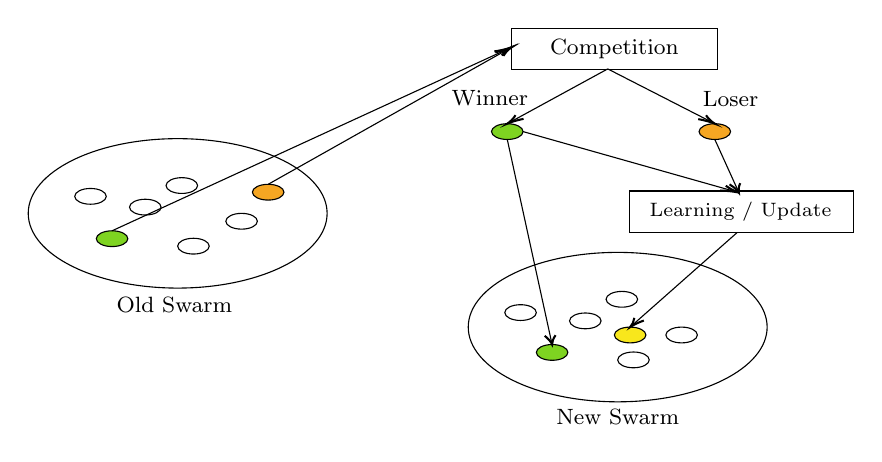
\begin{tikzpicture}[x=0.75pt,y=0.75pt,yscale=-0.4,xscale=0.8]
%uncomment if require: \path (0,621.0500030517578); %set diagram left start at 0, and has height of 621.0500030517578

%Shape: Circle [id:dp6268278507606896] 
\draw   (141,302) .. controls (141,252.29) and (181.29,212) .. (231,212) .. controls (280.71,212) and (321,252.29) .. (321,302) .. controls (321,351.71) and (280.71,392) .. (231,392) .. controls (181.29,392) and (141,351.71) .. (141,302) -- cycle ;
%Shape: Rectangle [id:dp3741559070244542] 
\draw   (432,79) -- (556,79) -- (556,129) -- (432,129) -- cycle ;
%Shape: Rectangle [id:dp38044702729098334] 
\draw   (503,275) -- (638,275) -- (638,325) -- (503,325) -- cycle ;
%Shape: Circle [id:dp9902831839272267] 
\draw   (169,281.5) .. controls (169,276.25) and (173.25,272) .. (178.5,272) .. controls (183.75,272) and (188,276.25) .. (188,281.5) .. controls (188,286.75) and (183.75,291) .. (178.5,291) .. controls (173.25,291) and (169,286.75) .. (169,281.5) -- cycle ;
%Shape: Circle [id:dp006483135953692765] 
\draw   (260,311.5) .. controls (260,306.25) and (264.25,302) .. (269.5,302) .. controls (274.75,302) and (279,306.25) .. (279,311.5) .. controls (279,316.75) and (274.75,321) .. (269.5,321) .. controls (264.25,321) and (260,316.75) .. (260,311.5) -- cycle ;
%Shape: Circle [id:dp24333263541974726] 
\draw   (224,268.5) .. controls (224,263.25) and (228.25,259) .. (233.5,259) .. controls (238.75,259) and (243,263.25) .. (243,268.5) .. controls (243,273.75) and (238.75,278) .. (233.5,278) .. controls (228.25,278) and (224,273.75) .. (224,268.5) -- cycle ;
%Shape: Circle [id:dp7601745941257889] 
\draw   (231,341.5) .. controls (231,336.25) and (235.25,332) .. (240.5,332) .. controls (245.75,332) and (250,336.25) .. (250,341.5) .. controls (250,346.75) and (245.75,351) .. (240.5,351) .. controls (235.25,351) and (231,346.75) .. (231,341.5) -- cycle ;
%Shape: Circle [id:dp4823144630313888] 
\draw   (202,294.5) .. controls (202,289.25) and (206.25,285) .. (211.5,285) .. controls (216.75,285) and (221,289.25) .. (221,294.5) .. controls (221,299.75) and (216.75,304) .. (211.5,304) .. controls (206.25,304) and (202,299.75) .. (202,294.5) -- cycle ;
%Shape: Circle [id:dp20072966432988004] 
\draw  [fill={rgb, 255:red, 126; green, 211; blue, 33 }  ,fill opacity=1 ] (182,332.5) .. controls (182,327.25) and (186.25,323) .. (191.5,323) .. controls (196.75,323) and (201,327.25) .. (201,332.5) .. controls (201,337.75) and (196.75,342) .. (191.5,342) .. controls (186.25,342) and (182,337.75) .. (182,332.5) -- cycle ;
%Shape: Circle [id:dp3629440455041728] 
\draw  [fill={rgb, 255:red, 245; green, 166; blue, 35 }  ,fill opacity=1 ] (276,276.5) .. controls (276,271.25) and (280.25,267) .. (285.5,267) .. controls (290.75,267) and (295,271.25) .. (295,276.5) .. controls (295,281.75) and (290.75,286) .. (285.5,286) .. controls (280.25,286) and (276,281.75) .. (276,276.5) -- cycle ;
%Shape: Circle [id:dp4816568188899374] 
\draw   (406,439) .. controls (406,389.29) and (446.29,349) .. (496,349) .. controls (545.71,349) and (586,389.29) .. (586,439) .. controls (586,488.71) and (545.71,529) .. (496,529) .. controls (446.29,529) and (406,488.71) .. (406,439) -- cycle ;
%Shape: Circle [id:dp9233426694577401] 
\draw   (428,421.5) .. controls (428,416.25) and (432.25,412) .. (437.5,412) .. controls (442.75,412) and (447,416.25) .. (447,421.5) .. controls (447,426.75) and (442.75,431) .. (437.5,431) .. controls (432.25,431) and (428,426.75) .. (428,421.5) -- cycle ;
%Shape: Circle [id:dp6811282209781646] 
\draw   (525,448.5) .. controls (525,443.25) and (529.25,439) .. (534.5,439) .. controls (539.75,439) and (544,443.25) .. (544,448.5) .. controls (544,453.75) and (539.75,458) .. (534.5,458) .. controls (529.25,458) and (525,453.75) .. (525,448.5) -- cycle ;
%Shape: Circle [id:dp42653013738199363] 
\draw   (489,405.5) .. controls (489,400.25) and (493.25,396) .. (498.5,396) .. controls (503.75,396) and (508,400.25) .. (508,405.5) .. controls (508,410.75) and (503.75,415) .. (498.5,415) .. controls (493.25,415) and (489,410.75) .. (489,405.5) -- cycle ;
%Shape: Circle [id:dp3596615023757278] 
\draw   (496,478.5) .. controls (496,473.25) and (500.25,469) .. (505.5,469) .. controls (510.75,469) and (515,473.25) .. (515,478.5) .. controls (515,483.75) and (510.75,488) .. (505.5,488) .. controls (500.25,488) and (496,483.75) .. (496,478.5) -- cycle ;
%Shape: Circle [id:dp0557771713953914] 
\draw   (467,431.5) .. controls (467,426.25) and (471.25,422) .. (476.5,422) .. controls (481.75,422) and (486,426.25) .. (486,431.5) .. controls (486,436.75) and (481.75,441) .. (476.5,441) .. controls (471.25,441) and (467,436.75) .. (467,431.5) -- cycle ;
%Shape: Circle [id:dp5508833691665627] 
\draw  [fill={rgb, 255:red, 126; green, 211; blue, 33 }  ,fill opacity=1 ] (447,469.5) .. controls (447,464.25) and (451.25,460) .. (456.5,460) .. controls (461.75,460) and (466,464.25) .. (466,469.5) .. controls (466,474.75) and (461.75,479) .. (456.5,479) .. controls (451.25,479) and (447,474.75) .. (447,469.5) -- cycle ;
%Shape: Circle [id:dp8274201082154569] 
\draw  [fill={rgb, 255:red, 248; green, 231; blue, 28 }  ,fill opacity=1 ] (494,448.5) .. controls (494,443.25) and (498.25,439) .. (503.5,439) .. controls (508.75,439) and (513,443.25) .. (513,448.5) .. controls (513,453.75) and (508.75,458) .. (503.5,458) .. controls (498.25,458) and (494,453.75) .. (494,448.5) -- cycle ;
%Straight Lines [id:da0605137142553851] 
\draw    (285.5,267) -- (430.67,103.5) ;
\draw [shift={(432,102)}, rotate = 491.6] [color={rgb, 255:red, 0; green, 0; blue, 0 }  ][line width=0.75]    (10.93,-3.29) .. controls (6.95,-1.4) and (3.31,-0.3) .. (0,0) .. controls (3.31,0.3) and (6.95,1.4) .. (10.93,3.29)   ;
%Straight Lines [id:da484264483957657] 
\draw    (191.5,323) -- (430.53,103.35) ;
\draw [shift={(432,102)}, rotate = 497.42] [color={rgb, 255:red, 0; green, 0; blue, 0 }  ][line width=0.75]    (10.93,-3.29) .. controls (6.95,-1.4) and (3.31,-0.3) .. (0,0) .. controls (3.31,0.3) and (6.95,1.4) .. (10.93,3.29)   ;
%Shape: Circle [id:dp9477214278184684] 
\draw  [fill={rgb, 255:red, 126; green, 211; blue, 33 }  ,fill opacity=1 ] (420,203.5) .. controls (420,198.25) and (424.25,194) .. (429.5,194) .. controls (434.75,194) and (439,198.25) .. (439,203.5) .. controls (439,208.75) and (434.75,213) .. (429.5,213) .. controls (424.25,213) and (420,208.75) .. (420,203.5) -- cycle ;
%Shape: Circle [id:dp4017746009314589] 
\draw  [fill={rgb, 255:red, 245; green, 166; blue, 35 }  ,fill opacity=1 ] (545,203.5) .. controls (545,198.25) and (549.25,194) .. (554.5,194) .. controls (559.75,194) and (564,198.25) .. (564,203.5) .. controls (564,208.75) and (559.75,213) .. (554.5,213) .. controls (549.25,213) and (545,208.75) .. (545,203.5) -- cycle ;
%Straight Lines [id:da23412320444772494] 
\draw    (490,128) -- (430.85,192.53) ;
\draw [shift={(429.5,194)}, rotate = 312.51] [color={rgb, 255:red, 0; green, 0; blue, 0 }  ][line width=0.75]    (10.93,-3.29) .. controls (6.95,-1.4) and (3.31,-0.3) .. (0,0) .. controls (3.31,0.3) and (6.95,1.4) .. (10.93,3.29)   ;
%Straight Lines [id:da009854351489168578] 
\draw    (490,128) -- (553.1,192.57) ;
\draw [shift={(554.5,194)}, rotate = 225.66] [color={rgb, 255:red, 0; green, 0; blue, 0 }  ][line width=0.75]    (10.93,-3.29) .. controls (6.95,-1.4) and (3.31,-0.3) .. (0,0) .. controls (3.31,0.3) and (6.95,1.4) .. (10.93,3.29)   ;
%Straight Lines [id:da6554616199613248] 
\draw    (568,325) -- (504.48,437.26) ;
\draw [shift={(503.5,439)}, rotate = 299.5] [color={rgb, 255:red, 0; green, 0; blue, 0 }  ][line width=0.75]    (10.93,-3.29) .. controls (6.95,-1.4) and (3.31,-0.3) .. (0,0) .. controls (3.31,0.3) and (6.95,1.4) .. (10.93,3.29)   ;
%Straight Lines [id:da7506472232160096] 
\draw    (439,203.5) -- (567.26,276.02) ;
\draw [shift={(569,277)}, rotate = 209.48] [color={rgb, 255:red, 0; green, 0; blue, 0 }  ][line width=0.75]    (10.93,-3.29) .. controls (6.95,-1.4) and (3.31,-0.3) .. (0,0) .. controls (3.31,0.3) and (6.95,1.4) .. (10.93,3.29)   ;
%Straight Lines [id:da6419954078244837] 
\draw    (554.5,213) -- (568.56,275.05) ;
\draw [shift={(569,277)}, rotate = 257.23] [color={rgb, 255:red, 0; green, 0; blue, 0 }  ][line width=0.75]    (10.93,-3.29) .. controls (6.95,-1.4) and (3.31,-0.3) .. (0,0) .. controls (3.31,0.3) and (6.95,1.4) .. (10.93,3.29)   ;
%Straight Lines [id:da5783865713926161] 
\draw    (429.5,213) -- (456.28,458.01) ;
\draw [shift={(456.5,460)}, rotate = 263.76] [color={rgb, 255:red, 0; green, 0; blue, 0 }  ][line width=0.75]    (10.93,-3.29) .. controls (6.95,-1.4) and (3.31,-0.3) .. (0,0) .. controls (3.31,0.3) and (6.95,1.4) .. (10.93,3.29)   ;

% Text Node
\draw (494,104) node   [align=left] {\footnotesize Competition};
% Text Node
\draw (419,163) node   [align=left] {\footnotesize Winner};
% Text Node
\draw (564,164) node   [align=left] {\footnotesize Loser};
% Text Node
\draw (570,300) node   [align=left] {\scriptsize Learning / Update};
% Text Node
\draw (229,412) node   [align=left] {\footnotesize Old Swarm};
% Text Node
\draw (496,547) node   [align=left] {\footnotesize New Swarm};

\end{tikzpicture}}
    \fbox{\includegraphics[scale=0.3]{CSO_Diagram.png}}
    \caption{Diagram adapted from Cheng and Jin (2015) that shows a general overview of the CSO. Particles are randomly grouped into pairs where they ``compete'' with each other. The winner is put into the new swarm, and the loser is updated before being placed into the new swarm.}
    \label{fig:cso}
\end{figure}

\begin{figure}[H]
    \renewcommand\figurename{Algorithm}
    \begin{algorithm}[H]
        \singlespacing
        \caption{Competitive Swarm Optimiser}
        \begin{algorithmic}[1]
            \For{$i = 1$ to $p$}
                \State{Initialise initial position, $\mb{x}_i$ and associated particle velocities $\mb{v}_i$}
            \EndFor
            \State{Initialise $t \leftarrow 0$}
            \State{Initialise $\bar{\mb{x}} \leftarrow \frac{1}{p} \sum_{i=1}^p \mb{x}_i$}
            \While{termination condition not reached}
                \State{Initialise $U_t$ as the set of all particles at iteration $t$}
                \State{Initialise $U_{t+1}$ as the set of all particles for the next iteration $t + 1$}
                \While{$U_t \neq \emptyset$}
                    \State{Randomly select $\mb{x}_i, \mb{x}_j \in U_t$}
                    \State{Remove $\mb{x}_i, \mb{x}_j$ from $U_t$}
                    \If{$f(\mb{x}_{i}) < f(\mb{x}_{j})$}
                        \State{$\mb{x}_w \leftarrow \mb{x}_i$, $\mb{x}_l \leftarrow \mb{x}_j$}
                    \Else
                        \State{$\mb{x}_w \leftarrow \mb{x}_j$, $\mb{x}_l \leftarrow \mb{x}_i$}
                    \EndIf
                    \State{Add $\mb{x}_w$ into $U_{t+1}$}
                    \State{Update loser velocity, $\mb{v}_l$}
                    \State{Update loser position, $\mb{x}_l \leftarrow \mb{x}_l + \mb{v}_l$}
                    \State{Add $\mb{x}_l$ into $U_{t+1}$}
                \EndWhile
                \State{$t \leftarrow t + 1$}
                \State{Update $\bar{\mb{x}} \leftarrow \frac{1}{p} \sum_{i=1}^p \mb{x}_i$ for $\mb{x}_i \in U_{t+1}$}.
            \EndWhile
        \end{algorithmic}
    \end{algorithm}
    \caption{The general procedure for the CSO algorithm based on  Cheng and Jin (2015).}
    \label{alg:cso}
\end{figure}

The initial particle positions and velocities are generated in the same way as described for that of the original PSO algorithm in Section \ref{subsection:pso algorithm}. The updating of the particle velocity is as follows:
$$\mb{v}_{l} \leftarrow \mb{R}_1 \circ \mb{v}_l + \mb{R}_2 \circ (\mb{x}_w - \mb{x}_l) + \phi \cdot \mb{R}_3 \circ (\bar{\mb{x}} - \mb{x}_l)$$
where $\mb{R}_1, \mb{R}_2, \mb{R}_3 \in \mathbb{R}^d$ are random vectors of i.i.d. $U(0, 1)$ uniform components, and the social factor $\phi \geq 0$ is a parameter that controls the contribution of the mean particle position $\bar{\mb{x}}$. The symbol $\circ$ denotes the Hadamard product. In the CSO, instead of all the particles being updated, only the loser particles are updated. In particular, setting $\phi = 0$ means that we ignore the other particles in the velocity update of the losers, and setting $\phi > 0$ will mean that the velocity update of the loser considers both the winner particle of that pair, and contributions from all other particles. \newline

Cheng and Jin provide a set of recommendations on how to select the number of particles $p$ and the social factor $\phi$ based on empirical results. For a function with dimension less than or equal to 500, we set $p = 100$ and $\phi = 0$, with values of $p$ and $\phi$ increasing as the dimension of the function increases. For the purposes of this thesis, all functions we consider will have dimension less than 500.

\subsection{Quantum-behaved Particle Swarm Optimisation}
Quantum-behaved Particle Swarm Optimisation (QPSO) proposed by Sun et. al (2004) \cite{sun2004} is another variant of the original PSO algorithm inspired by quantum mechanics. Each particle is treated as a spin-less particle moving in a $d$-dimensional quantum space characterised by a wave function $\psi$, where $d$ is the dimension of the function $f$ to be minimised, and are updated by assuming that the particles moves in the $d$-dimensional quantum space with a $\delta$ potential well.
\newline

On top of the notation used in Section \ref{subsection:pso algorithm}, we include some additional definitions: $\bar{\mb{x}}^b$ denotes the mean of all the personal best particle positions in the swarm, and $\bar{x}^b_j$ denotes the $j^\text{th}$ dimension of the mean of all personal best particle positions. The QPSO algorithm is given in Algorithm \ref{alg:qpso}.

\begin{figure}[H]
    \renewcommand\figurename{Algorithm}
    \begin{algorithm}[H]
        \singlespacing
        \caption{Quantum-behaved Particle Swarm Optimisation}
        \begin{algorithmic}[1]
            \For{$i = 1$ to $p$}
                \State{Initialise initial position, $\mb{x}_i$}
                \State{Initialise particle velocity, $\mb{v}_i$}
                \State{Set particle best position to initial position, $\mb{x}^b_i \leftarrow \mb{x}_i$}
                \If{$f(\mb{x}^b_i) < f(\mb{x}^g)$}
                    \State{Update global best position, $\mb{x}^g \leftarrow \mb{x}^b_i$}
                \EndIf
            \EndFor
            \State{Initialise $\bar{\mb{x}}^b \leftarrow \frac{1}{p} \sum_{i=1}^p \mb{x}^b_i$}
            \While{termination condition not reached}
                \For{$i = 1$ to $p$}
                    \For{$j = 1$ to $d$}
                        \State{Generate $u_{1,j}, u_{2,j}, u_{3,j} \overset{i.i.d.}{\sim} U(0, 1)$}
                        \State{Let $y_j \leftarrow u_{1,j} \cdot x^b_{i,j} + (1 - u_{1,j}) \cdot \mb{x}^g_j$}
                        \State{Update particle position $x_{i,j}$}  
                    \EndFor
                \EndFor
                \If{$f(\mb{x}_i) < f(\mb{x}^b_i)$}
                    \State{Update particle best position, $\mb{x}^b_i \leftarrow \mb{x}_i$}
                    \If{$f(\mb{x}^b_i) < f(\mb{x}^g)$}
                        \State{Update global best position, $\mb{x}^g \leftarrow \mb{x}^b_i$}
                    \EndIf
                \EndIf
                \State{Update $\bar{\mb{x}}^b \leftarrow \frac{1}{p} \sum_{i=1}^p \mb{x}^b_i$}
            \EndWhile
        \end{algorithmic}
    \end{algorithm}
    \caption{The general procedure for the QPSO algorithm based on Sun et. al (2004).}
    \label{alg:qpso}
\end{figure}

The initial particle positions and velocities are generated in the same way as described for that of PSO in Section \ref{subsection:pso algorithm}. There are two variants of the particle position update procedure for QPSO \cite{1460396, Sun2012ConvergenceAA}. The QPSO-Type 1 (QPSO-T1) has the following update procedure:
$$x_{i,j} \leftarrow 
\begin{cases}
y_j + \alpha \cdot \lvert x_{i,j} - y_j \rvert \cdot \ln{(1 / u_{2,j})}, & \text{if} \ u_{3,j} < 0.5, \\
y_j - \alpha \cdot \lvert x_{i,j} - y_j \rvert \cdot \ln{(1 / u_{2,j})}, & \text{otherwise} \ . \\
\end{cases}$$
Alternatively, the QPSO-Type 2 (QPSO-T2) has the following update procedure:
$$x_{i,j} \leftarrow 
\begin{cases}
y_j + \alpha \cdot \lvert x_{i,j} - \bar{x}^b_j \rvert \cdot \ln{(1 / u_{2,j})}, & \text{if} \ u_{3,j} < 0.5, \\
y_j - \alpha \cdot \lvert x_{i,j} - \bar{x}^b_j \rvert \cdot \ln{(1 / u_{2,j})}, & \text{otherwise} \ . \\
\end{cases}$$
The two different update procedures differ in the additional contribution from the mean best particle positions in the swarm for QPSO-T1 instead of just the value $y_j$. The value $y_j$ is a randomly weighted average of the particle's best position and the global best position for dimension $j$. Thus, the update of the particle position takes in the contribution from the particle's best position and the global best position for both the QPSO-T1 and QPSO-T2. The contraction-expansion coefficient $\alpha > 0$ is a parameter that controls the balance between the global search and local search of the algorithm.

\subsection{Comparison of Update Procedures}
We can compare the difference in the velocity update in CSO to that of the original PSO algorithm. The first term that controls the effect from the previous velocity still remains, but it is now scaled randomly instead of by a constant $w$. The second term that was the cognitive component in the PSO is now replaced by the learning component in the CSO, where the particle is updated with contribution from the particle that won against it. The third term that was the social component also remains, but now instead of the contribution from the global best, it is now the contribution from the mean position of all the particles in the swarm. \newline

Unlike both the PSO and CSO, QPSO is not dependent on the update of a velocity term to update the particle position. It is instead updated directly by the particle positions of itself, its previous best, the global best, and other particle positions. In the QPSO, the update is also dependent on a uniform random variable, which is emulating the flipping of a unbiased coin, to determine whether the update should be the addition or subtraction of the second term to $y_j$.

\newpage

\section{Enhancements of Particle Swarm Optimisation}
\label{section:enhancements}
This section will discuss two new enhancements to the original PSO algorithm, the Smoothed Particle Swarm Optimisation and the Adaptive Smoothed Particle Swarm Optimisation \cite{choi2020}, that aims to address the problem of non-convergence of the original PSO algorithm discussed in Section \ref{subsection:pso non-convergence}.

\subsection{Smoothed Particle Swarm Optimisation}
\label{subsection:spso algorithm}
The original PSO algorithm faces the problem of ``swarm collapse'' where all the particles may converge to a single point, which may not be the global minimum. At this point, any attempts to update the particle positions will not result in any significant changes to the particle positions. Smoothed Particle Swarm Optimisation (sPSO) tries to address this problem by introducing two new parameters $\eta$ and $\sigma$ with a modification of the update procedure in the original PSO algorithm. The sPSO algorithm has ensured convergence to the global minimum, and the results of the proof are discussed in Section \ref{subsection:convergence results}. \newline

The sPSO algorithm follows exactly the same general procedure as that of PSO as outlined in Section \ref{subsection:pso algorithm}, with the only difference being the update procedure of the particle velocity $v_{i, j}$ for the $i^\text{th}$ particle at the $j^\text{th}$ dimension. The sPSO update procedure is as follows:
$$v_{i,j} \leftarrow (1 - \eta w) \cdot v_{i,j} + \eta \cdot c_1 \cdot u_{b,j} \cdot  (x^b_{i,j} - x_{i,j}) + \eta \cdot c_2 \cdot u_{g,j} \cdot (x^g_j - x_{i,j}) + \eta \cdot \sigma \cdot Z$$
where $Z \overset{i.i.d.}{\sim} N(0, 1)$ is a standard normal random variable, and $0 < \eta \leq 1$ and $\sigma \geq 0$ are new parameters introduced by sPSO. Here, the values of $c_1, c_2 > 0$ refer to the same cognitive and social coefficients in PSO respectively. However, the value of $w$ for sPSO does not refer to the same inertia weight value $w$ in PSO. If we were to denote the intertia weight in PSO as $w^*$, then the analogous equivalent of intertia weight would be $w = 1 - w^*$ in sPSO. In this way, we can view PSO as a special case of sPSO with $\eta = 1$ and $\sigma = 0$. \newline

An additional standard normal random variable $Z$ is included in the update step for sPSO, which corresponds to adding noise to the velocity update. Specifically, we consider $\sigma \cdot Z$, which corresponds to a normal random variable with mean $0$ and variance $\sigma^2$. The addition of the normally distributed noise is to help prevent the particles from premature convergence, by ensuring that there will still be changes to the velocity and thus the particle positions even for particles which are at their personal or global best positions. \newline

The parameter $\eta$ acts as a step size. It reduces the contribution to the velocity from the social and cognitive terms in the velocity update, while increasing the contribution from the previous particle velocity. In particular, we can rewrite the velocity update step as
$$v_{i,j} \leftarrow  (1 - \eta w) \cdot v_{i,j} +  \eta \left( c_1 \cdot u_{b,j} \cdot  (x^b_{i,j} - x_{i,j}) + c_2 \cdot u_{g,j} \cdot (x^g_j - x_{i,j}) + \sigma \cdot Z \right)$$
which shows more clearly the effect of $\eta$ on the entire velocity update. Decreasing the value of $\eta$ would increase the value of $1 - \eta w$, increasing the contribution from the previous velocity $v_{i,j}$, while decreasing the contribution from all the other terms. The reduction in velocity for the social and cognitive factors here is similar to the concept of constriction factors, with the difference that the multiplicative factor is not dependent on $c_1$ and $c_2$. We can see $\eta$ as a parameter that helps to balance the \textit{Exploration-Exploitation Tradeoff}. A smaller value of $\eta$ is analogous to focusing on exploration, since we are trying to penalise exploitation by reducing the contribution from the personal and global bests. A larger value of $\eta$ would mean that we are focusing on exploitation by making greater use of the knowledge from the personal and global best positions.

% smaller change in particle velocity at each iteration, which can be seen as the particles ``moving more slowly''. The slower movement can help prevent particles from moving too far from its previous position, which may cause it to miss parts of the search space that could have given better candidate solutions. Thus, the inclusion of $\eta$ leads to a ``smoothing'' effect on the particle movement by reducing the overall velocity and thus making the movement of each particle smaller.

\subsection{Adaptive Smoothed Particle Swarm Optimisation}
\label{subsection:apso algorithm}
Although sPSO has guaranteed convergence to the global minimum compared to PSO, the smaller particle velocities and thus smaller movements may result in sPSO taking many more iterations to converge than PSO does. The inclusion of $\sigma$ may also result in the algorithm moving away from a good candidate solution. Adaptive Smoothed Particle Swarm Optimisation (aPSO) addresses this by introducing a data-driven framework for the parameters $\eta$ and $\sigma$ instead of keeping them at a fixed constant in sPSO. Like sPSO, aPSO has guaranteed convergence to the global minimum, and the results of the proof are discussed in Section \ref{subsection:convergence results}. \newline

We introduce $C_t$, a measure of the algorithm stagnation. Let $t$ denote the current iteration number, and $\mb{x}^g(k)$ denote the global best particle position at iteration $k$. We define $C_t = \min \left\{1, \max \left\{\frac{t - \psi_t}{T_s} - 1, 0 \right\}\right\}$, where $\psi_t = \max \left\{s \leq t: \mb{x}^g(s) \neq \mb{x}^g(s-1) \right\}$ is the last iteration number that $\mb{x}^g$ has been updated, and $T_s$ is an iteration threshold. Thus $t - \psi_t$ is the number of iterations that $\mb{x}^g$ has remained unchanged, and the value of $C_t$ becomes greater than $0$ only after $t - \psi_t > T_s$. Thus, the algorithm is treated as stagnated only after $C_t$ becomes positive. \newline

On top of $C_t$, since $\eta$ and $\sigma$ are no longer constant values, we define a range of values that the parameters can take. For any iteration $t$, the values $\eta_t$ and $\sigma_t$ can also vary for each iteration, such that $\eta_t \in \left[\eta_\text{min}, \eta_\text{max}\right]$ and $\sigma_t \in \left[\sigma_\text{min}, \sigma_\text{max}\right]$, denoting the upper and lower bounds for both parameters that are to be defined, such that $0 \leq \eta_\text{min} \leq \eta_t \leq \eta_\text{max}$ and $0 \leq \sigma_\text{min} \leq \sigma_t \leq \sigma_\text{max}$. The aPSO algorithm is given in Algorithm \ref{alg:apso}.

\begin{figure}[H]
    \renewcommand\figurename{Algorithm}
    \begin{algorithm}[H]
        \singlespacing
        \caption{Adaptive Smoothed Particle Swarm Optimisation}
        \begin{algorithmic}[1]
            \For{$i = 1$ to $p$}
                \State{Initialise initial position, $\mb{x}_i$}
                \State{Initialise particle velocity, $\mb{v}_i$}
                \State{Set particle best position to initial position, $\mb{x}^b_i \leftarrow \mb{x}_i$}
                \If{$f(\mb{x}^b_i) < f(\mb{x}^g)$}
                    \State{Update global best position, $\mb{x}^g \leftarrow \mb{x}^b_i$}
                \EndIf
            \EndFor
            \State{Initialise $t = 0$}
            \State{Initialise $\tau = 0$}
            \While{termination condition not reached}
                \State{Update $t \leftarrow t + 1$}
                \State{Update $C_t \leftarrow \min \left\{1, \max \left\{\frac{\tau}{T_s} - 1, 0 \right\}\right\}$}
                \State{Calculate $\sigma_t, \eta_t$}
                \State{Initialise \textit{updated} $\leftarrow$ \textbf{False}}
                \For{$i = 1$ to $p$}
                    \For{$j = 1$ to $d$}
                        \State{Generate $u_{b,j}, u_{g,j} \overset{i.i.d.}{\sim} U(0, 1)$}
                        \State{Update particle velocity $v_{i,j}$}
                    \EndFor
                    \State{Update particle position $\mb{x}_i \leftarrow \mb{x}_i + \mb{v}_i$}
                    \If{$f(\mb{x}_i) < f(\mb{x}^b_i)$}
                        \State{Update particle best position, $\mb{x}^b_i \leftarrow \mb{x}_i$}
                        \If{$f(\mb{x}^b_i) < f(\mb{x}^g)$}
                            \State{Update global best position, $\mb{x}^g \leftarrow \mb{x}^b_i$}
                            \State{\textit{updated} $\leftarrow$ \textbf{True}}
                        \EndIf
                    \EndIf
                \EndFor
            \If{\textit{updated} is \textbf{True}}
                \State{Set $\tau \leftarrow 0$}
            \Else
                \State{Update $\tau \leftarrow \tau + 1$}
            \EndIf
            \EndWhile
        \end{algorithmic}
    \end{algorithm}
    \caption{The general procedure for the aPSO algorithm.}
    \label{alg:apso}
\end{figure}

Like the other algorithms, the initial particle positions and velocities are generated as per PSO in Section \ref{subsection:pso algorithm} and $\tau = t - \psi_t$ represents the number of iterations of stagnation, and is used here to simplify the algorithm. The parameters $\sigma_t$ and $\eta_t$ are calculated as follows:
$$\begin{aligned}
\sigma_t &\rightarrow \sigma_\text{max} C_t + \sigma_\text{min} (1 - C_t) \\
\eta_t &\rightarrow \eta_\text{min} C_t + \eta_\text{max} (1 - C_t) \\
\end{aligned}$$
Since $C_t \in [0, 1]$, $\sigma_t$ and $\eta_t$ can be viewed as either a linear combination or a weighted average of their corresponding upper and lower bounds. Thus, $\sigma_t$ increases and $\eta_t$ decreases whenever the value of $C_t$, or stagnation, increases. \newline

The update procedure for aPSO is of the same form as that of sPSO. The update procedure is as follows:
$$\begin{aligned}
v_{i,j} &\leftarrow (1 - \eta_t w) \cdot v_{i,j} + \eta_t \cdot c_1 \cdot u_{b,j} \cdot  (x^b_{i,j} - x_{i,j}) + \eta_t \cdot c_2 \cdot u_{g,j} \cdot (x^g_j - x_{i,j}) + \eta_t \cdot \sigma_t \cdot Z
\end{aligned}$$
Thus, the only difference in the update procedure is replacing the constants $\sigma$ and $\eta$ parameters with the adaptive parameters $\sigma_t$ and $\eta_t$. \newline

Consider the particular case where $\eta_\text{min} = 0$, $\eta_\text{max} = 1$, $\sigma_\text{min} = 0$ and $\sigma_\text{max} = 1$. When there is no stagnation, i.e. $C_t = 0$, we have $\sigma_t = 0$ and $\eta_t = 1$ exactly, corresponding to the PSO. When $C_t = \epsilon$, where $0 < \epsilon < 1$, we have $\sigma_t = \epsilon$ and $\eta_t = 1 - \epsilon$, corresponding to the sPSO. Thus, we can view the aPSO as a combination of both the original PSO and sPSO, or the algorithm ``switching'' between the two algorithms. In the initial stages of the algorithm where there is no stagnation, $C_t = 0$ and the algorithm simplifies to PSO. When $C_t > 0$ and stagnation occurs, the algorithm does a ``switch'' to sPSO by reducing $\eta_t$ and increasing $\sigma_t$. Again, we can view this as balancing the \textit{Exploration-Exploitation Tradeoff} as discussed for sPSO in Section \ref{subsection:spso algorithm}. When there is no stagnation, the algorithm focuses on exploiting the information available to improve the solution. When stagnation occurs, the algorithm will start to explore other parts of the search space to find other possibly better solutions.

\subsection{Convergence Results}
\label{subsection:convergence results}
Compared to PSO which may not converge to the global minimum due to ``swarm collapse', sPSO and aPSO has guaranteed convergence to the global minimum. The proof of convergence of can be found in Choi et. al \cite{choi2020}. The full proof will not be discussed here as it is beyond the scope of this project. We will discuss some of the assumptions and results of the proof in this section.

\begin{definition}
For a function $f:\mathbb{R}^n \rightarrow \mathbb{R}$, $f$ is coercive if $\underset{\lVert \mb{x} \rVert \rightarrow \infty}\lim f(\mb{x}) = \infty$.
\end{definition}

It is important that we assume that our objective function is coercive, so that the global minimum exists. For example, consider the function  $f(x) = -x$, which is not coercive. As $x \rightarrow \infty$, $f(x) \rightarrow -\infty$ and $f$ has no global minimum.

\begin{theorem}
\label{theorem:spso convergence}
Suppose $f$ is a continuous function that is coercive. There exists $\eta_0$ such that for all $\eta$, where $0 < \eta \leq \eta_0$, such that the following statements are true.
\begin{enumerate}[(i)]
    \item The sPSO algorithm is stochastically bounded:
    $$\underset{t \rightarrow \infty}{\lim \sup} \ \mathbb{E} \lVert \mb{x}_i(t) \rVert^2 < \infty, \
    \underset{t \rightarrow \infty}{\lim \sup} \ \mathbb{E} \lVert \mb{v}_i(t) \rVert^2 < \infty.$$
    \item The sPSO algorithm will eventually find the global optimum:
    $$\underset{t \rightarrow \infty}{\lim} f(\mb{x}^g(t)) = \underset{\mb{x}}{\min} f(\mb{x}).$$
\end{enumerate}
\end{theorem}

Here, $\mb{x}_i(t)$ and $\mb{v}_i(t)$ denote the particle position and velocity of the $i^\text{th}$ particle at iteration $t$, and $\mb{x}^g(t)$ denotes the global best particle position at iteration $t$. Theorem \ref{theorem:spso convergence} provides a convergence result for the sPSO in the limit. However, it is important to note that the number of iterations required for convergence may be extremely large.

\begin{theorem}
\label{theorem:apso convergence}
Suppose $f$ is a continuous function that is coercive, and there are constants $0 < \eta_- < \eta_+ \leq 1$ and $0 < \sigma_- < \sigma_+$ such that the parameter choices satisfy
$$\eta_- \leq \eta_t \leq \eta_+, \ \sigma_- \leq \sigma_t \leq \sigma_+.$$
Also assume that there exists an interior point $\mb{x}^* \in \mathcal{D}$, where $\mathcal{D}$ is the search space of the algorithm which is a closed and bounded set, such that $f(\mb{x}^*) = \underset{\mb{x}}{\min} f(\mb{x})$. There exists $M$ such that for all $\mb{x} \in D, \ \lVert \mb{x} \rVert \leq M$, such that the following statements are true.
\begin{enumerate}[(i)]
    \item The aPSO algorithm is stochastically bounded:
    $$\lVert \mb{x}_i(t) \rVert^2 < M^2, \
    \underset{t \rightarrow \infty}{\lim \sup} \ \mathbb{E} \lVert \mb{v}_i(t) \rVert^2 < \infty.$$
    \item The aPSO algorithm will eventually find the global optimum:
    $$\underset{t \rightarrow \infty}{\lim} f(\mb{x}^g(t)) = \underset{\mb{x}}{\min} f(\mb{x}).$$
\end{enumerate}
\end{theorem}

Theorem \ref{theorem:apso convergence} provides a convergence result for aPSO that is stronger than that of sPSO. In particular, by considering $\eta_t = \eta$ and $\sigma_t = \sigma$ in our assumptions for Theorem \ref{theorem:apso convergence}, we can view sPSO as a special case of aPSO.

\subsection{Effect of Parameter Choices on sPSO and aPSO}
\label{subsection:parameter choices}
To investigate the effect of the two new parameters in sPSO $\eta$ and $\sigma$, sPSO was run on 30 test functions for 100 repetitions, each for 10,000 iterations, to obtain the estimate of the global minimum for varying levels of $\eta$ and $\sigma$, and the mean of the 100 estimates were calculated. The 30 test functions are discussed further in Section \ref{subsection:test functions} and are also found in Appendix \ref{subsection:function info}. The algorithm is initialised with 32 particles. For the parameter values, we considered $\eta \in \left\{ 0.025, 0.05, 0.1, 0.2, 0.4, 0.8 \right\}$ and $\sigma \in \left\{ 0.5, 1, 2, 4, 8 \right\}$. The results are shown in Appendix \ref{subsection:parameter spso}. Table \ref{tab:spso winners table} shows the number of times a particular $\eta$ and $\sigma$ pair obtains the smallest mean for a particular function and dimension. \newline

\begin{table}[H]
    \centering
    \renewcommand{\arraystretch}{0.7}
    \begin{tabular}{|l|l|l|l|l|l|}
\toprule
\diagbox{$\eta$}{$\sigma$} & 0.5 & 1 & 2 & 4 & 8 \\
\midrule
0.025 & 25  & 0 & 0 & 0 & 0 \\ \midrule
0.05  & 17  & 2 & 0 & 0 & 0 \\ \midrule
0.1   & 7   & 0 & 1 & 0 & 0 \\ \midrule
0.2   & 4   & 1 & 0 & 0 & 0 \\ \midrule
0.4   & 3   & 0 & 2 & 0 & 0 \\ \midrule
0.8   & 3   & 2 & 1 & 0 & 3 \\
\bottomrule
\end{tabular}
    \renewcommand{\arraystretch}{1}
    \caption{Table of results showing number of times each $\eta$ and $\sigma$ pair obtain the smallest mean estimate of the global minimum for the 30 test functions across varying dimensions. Of the 75 function-dimension pairs, 4 are not included due to ties.}
    \label{tab:spso winners table}
\end{table}

The results show a general trend of sPSO performing better with smaller values of $\eta$ and smaller values of $\sigma$. Specifically, the $(\eta, \sigma)$ pairs of $(0.025, 0.5)$ and $(0.05, 0.5)$ perform the best across the 30 test functions with varying dimension. \newline

Similarly, we also investigate the effect of the parameters in aPSO in a similar setup to that done for sPSO. Here we fix $\eta_\text{max} = 1$ and $\sigma_\text{min} = 0.01$, and vary $\eta_\text{min}$ and $\sigma_\text{max}$, where $\eta_\text{min} \in \left\{ 0.025, 0.05, 0.1, 0.2, 0.4, 0.8 \right\}$ and $\sigma_\text{max} \in \left\{ 0.5, 1, 2, 4, 8 \right\}$. Here, fixing $\eta_\text{max} = 1$ is a logical choice as it is the maximum upper bound possible for any value of $\eta$, while fixing $\sigma_\text{min} = 0.01$ is a small enough value that such that any contribution from the normal term in the velocity update step will be extremely small. The results are shown in Appendix \ref{subsection:parameter apso}. \newline

The results show that there is very little effect on the performance of aPSO when varying $\eta_\text{min}$ and $\sigma_\text{max}$. For varying dimensions of the test functions, there are mostly no differences in the mean of the estimates obtained at different values of $\eta$ and $\sigma$, with any differences being of a very small magnitude, such as the results for F1, F2, F3 and F4. Note that only the results for F1 to F10 are shown in Appendix \ref{subsection:parameter apso}, but the general trend persists for F11 to F30.

\subsection{Comparing Empirical Convergence of PSO, sPSO, aPSO}
\label{subsection:empirical convergence}
We investigated the performance of PSO and the two PSO enhancements, sPSO and aPSO. The three algorithms were run for 100 repetitions, each of 500,000 iterations, on 8 test functions to obtain the estimates of the global minimum, and the mean and standard deviation of the 100 estimates were calculated. All three algorithms were initialised with 32 particles. For sPSO, the parameter values were chosen to be $\eta = 0.025$ and $\sigma = 0.5$. For aPSO, the parameter values were chosen to be $\eta_\text{min} = 0.025$, $\eta_\text{max} = 1$, $\sigma_\text{min} = 0.01$ and $\sigma_\text{max} = 0.5$. The results are shown in Table \ref{tab:500k table}.

\begin{table}[H]
    \centering
    \renewcommand{\arraystretch}{0.7}
    \begin{tabular}{|l|l|l|l|l|l|}
\hline
Function     & Dim & Min & PSO                    & sPSO             & aPSO             \\ \hline
Ackley       & 40 & 0 & 16.18(6.227)          & 16.06(1.819)    & 15.93(6.911)    \\ \hline
Bohachevsky1 & 40 & 0 & 1.48e+4(1.79e+4)   & 10.53(2.559)    & 0.359(0.031)     \\ \hline
Bohachevsky2 & 40 & 0 & 1.45e+4(1.77e+4)   & 4.072(0.512)     & 0.291(0.024)     \\ \hline
Eggholder    & 2 & -959.6 & -930.5(60.19)       & -950.3(30.04) & -931.9(59.82) \\ \hline
Griewank     & 40 & 0 & 50.67(62.01)         & 0.014(0.014)     & 0.066(0.092)     \\ \hline
Rastrigin    & 40 & 0 & 218.8(45.44)        & 203.0(45.24)    & 111.7(40.72)   \\ \hline
Rosenbrock   & 40 & 0 & 2.30e+5(4.22e+5) & 126.1(197.0) & 78.46(76.80)   \\ \hline
Sumsquare    & 40 & 0 & 355.2(319.7)       & 2.111(0.232)     & 0.14(0.014)      \\ \hline
\end{tabular}
    \renewcommand{\arraystretch}{1}
    \caption{Table of 8 test functions and their corresponding dimension, with the averaged results for 100 repetitions of 500,000 iterations for the three algorithms: PSO, sPSO and aPSO. The first value in each cell is the mean, followed by the standard deviation given in brackets.}
    \label{tab:500k table}
\end{table}

From the results, aPSO obtains a mean that is the closest to the global minimum for the 8 test functions, except for Eggholder and Griewank, where the mean for sPSO is the closest to the global minimum. The improvement in performance from PSO to sPSO and PSO to aPSO is especially substantial for some functions such as Bohachevsky1, Bohachevsky2, Griewank, Rosenbrock and Sumsquare, where the mean is several orders of magnitude smaller. The improvement in performance from sPSO to aPSO is still significant although smaller than that from PSO to sPSO. For example, the mean for Bohachevsky1 reduced by close to 1500 times and 30 times respectively from PSO to sPSO and sPSO to aPSO. \newline

In addition to the final estimates of the results, we also consider the estimates obtained during the algorithm. For each of the algorithms, the global best estimates were taken at the following iteration numbers: 10, 50, 100, 200, 400, 1000, 3000, 10000, 100000 and 5000000, which is the last iteration. The respective average of the global best values are plotted against a log-scale of the iteration numbers for clarity and are shown in Figure \ref{fig:500k graphs}. \newline

The graphs provide a clearer picture of the similarities and differences in the behavior of the three algorithms. The average global best values for sPSO are always decreasing at a slower rate than that of PSO. However, the average global best value of PSO tends to become completely stagnant earlier, while the for sPSO the values usually continue decreasing and become stagnant at a value lower than that of PSO. This illustrates the fact that the sPSO takes a longer time to converge due to the smaller velocities compared to PSO. \newline

For aPSO, the average global best values obtained follow a trajectory that is very similar to that of PSO. However, in most cases where the values for PSO becomes stagnant, the values for aPSO continue to decrease, in a trajectory that is similar to that of sPSO. This illustrates the ``switch'' from PSO to sPSO mentioned in Section \ref{subsection:apso algorithm}, as the values start to become stagnant.

\begin{figure}[H]
    \centering
    \includegraphics[height=0.35\textwidth,width=.45\textwidth]{gbests/Ackley_500k.eps} \quad
    \includegraphics[height=0.35\textwidth,width=.45\textwidth]{gbests/Bohachevsky1_500k.eps}
    \medskip
    
    \includegraphics[height=0.35\textwidth,width=.45\textwidth]{gbests/Bohachevsky2_500k.eps} \quad
    \includegraphics[height=0.35\textwidth,width=.45\textwidth]{gbests/Eggholder_500k.eps}
    \medskip
    
    \includegraphics[height=0.35\textwidth,width=.45\textwidth]{gbests/Griewank_500k.eps} \quad
    \includegraphics[height=0.35\textwidth,width=.45\textwidth]{gbests/Rastrigin_500k.eps}
    \medskip
    
    \includegraphics[height=0.35\textwidth,width=.45\textwidth]{gbests/Rosenbrock_500k.eps} \quad
    \includegraphics[height=0.35\textwidth,width=.45\textwidth]{gbests/Sumsquare_500k.eps}
    
    \caption{Graphs of performance of PSO, sPSO and aPSO for the 8 test functions. The $x$-axis is the number of iterations in $\log$ scale, and the $y$-axis is the average global best value.}
    \label{fig:500k graphs}
\end{figure}

Another method to compare the three algorithms would be to consider first-order stochastic dominance \cite{hadar1969rules}. For two probability distributions $f$ and $g$ with the same support $X$, and respective Cumulative Distribution Function (CDF) $F(x)$ and $G(x)$, $f$ first-order stochastically dominates $g$ if and only if $F(x) \leq G(x)$ for all $x \in X$. This can be verified graphically by plotting $F(x)$ and $G(x)$ to check if the two curves intersect. \newline

We can treat each result from 100 repetitions of an algorithm on a test function as i.i.d. random variables from the same distribution and compute the empirical CDF for the algorithm, and compare the empirical CDF from different algorithms. We consider two algorithms A and B with empirical CDF $F_A$ and $F_B$ respectively. If $F_A(x) \leq F_B(x)$ for all $x$, A first-order stochastically dominates B. Thus, $B$ would be the better algorithm, since the empirical probability that we will obtain a lower value that is closer to the global minimum is always greater. In particular, a good algorithm would have a empirical CDF that is close to a vertical line, meaning that the probability of obtaining a solution close to the global minimum would be close to 1. The empirical CDFs for the 8 test functions at three iteration numbers, 1000, 10000 and 500000, are shown in Figure \ref{fig:ecdf graphs}. \newline

Looking at the rightmost graph of each row in Figure \ref{fig:ecdf graphs}, we can see that for most of the functions, both sPSO and aPSO obtain a empirical CDF that is close to vertical. In these cases, we can see that PSO first-order stochastically dominates the other two algorithms. For Rastrigin, despite none of the empirical CDFs being vertical, the CDFs do not intersect, and PSO stochastically dominates sPSO and aPSO, while sPSO stochastically dominates aPSO. For Ackley and Eggholder, since the CDFs intersect, we cannot conclude that one algorithm stochastically dominates any other algorithm. \newline

As the number of iterations increase from 1000 to 10000 and to 500000, we can see a general trend that the empirical CDF for sPSO is moving towards the left and becoming closer to the empirical CDF of sPSO, and can be seen in the graphs for Bohachevsky1, Bohachevsky2, Griewank, Rastrigin, Rosenbrock and Sumsquare. As the number of iterations increase, sPSO is still able to improve on the estimate of the global minimum, while the PSO becomes stagnant. The empirical CDF of aPSO starts out having a higher degree of overlap with the empirical CDF of PSO. As the number of iterations increases, the degree of overlap becomes smaller, and the empirical CDF of aPSO overlaps more with the empirical CDF of sPSO. Once again, this illustrates the ``switch'' from PSO to sPSO mentioned in Section \ref{subsection:apso algorithm}. \newline

Overall, the results from Figure \ref{fig:ecdf graphs} agree with the results from Figure \ref{fig:500k graphs} that the aPSO and sPSO have better performance than that of PSO.

\begin{figure}[H]
    \centering
    \includegraphics[height=0.33\textwidth,width=\textwidth]{ecdfs/Ackley_500k.eps} \\ \bigskip
    \includegraphics[height=0.33\textwidth,width=\textwidth]{ecdfs/Bohachevsky1_500k.eps} \\ \bigskip
    \includegraphics[height=0.33\textwidth,width=\textwidth]{ecdfs/Bohachevsky2_500k.eps} \\ \bigskip
    \includegraphics[height=0.33\textwidth,width=\textwidth]{ecdfs/Eggholder_500k.eps}
    \caption{Graphs of Empirical CDF of PSO, sPSO and aPSO for the 8 test functions. The $x$-axis is the global best value of the results, and the $y$-axis is the cumulative probability. Each row contains the plots for the 500, 10000 and 500000 iterations respectively for each function.}
    \label{fig:ecdf graphs}
\end{figure}
    
\begin{figure}[H]
    \ContinuedFloat
    \includegraphics[height=0.33\textwidth,width=\textwidth]{ecdfs/Griewank_500k.eps} \\ \bigskip
    \includegraphics[height=0.33\textwidth,width=\textwidth]{ecdfs/Rastrigin_500k.eps} \\ \bigskip
    \includegraphics[height=0.33\textwidth,width=\textwidth]{ecdfs/Rosenbrock_500k.eps} \\ \bigskip
    \includegraphics[height=0.33\textwidth,width=\textwidth]{ecdfs/Sumsquare_500k.eps}
    \caption{Graphs of Empirical CDF of PSO, sPSO and aPSO for the 8 test functions. The $x$-axis is the global best value of the results, and the $y$-axis is the cumulative probability. Each row contains the plots for the 500, 10000 and 500000 iterations respectively for each function.}
    % \caption{Graphs of performance of PSO, sPSO and aPSO for the 8 test functions. The $x$-axis is the number of iterations in $\log$ scale, and the $y$-axis is the average function value of the global best positions. Each row contains the plots for the 500, 10000 and 500000 iterations respectively for each function.}
\end{figure}

\newpage

\section{Comparative Studies of Swarm Algorithms}
\label{section:comparative studies}
In this section, we compare the performance of PSO with its enhancements and variants on a suite of test functions. Specifically, we compare the performance of the original PSO, sPSO and aPSO introduced in Section \ref{section:enhancements}, and CSO and QPSO (both QPSO-T1 and QPSO-T2) introduced in Section \ref{section:related swarm algo}. All experiments are run on MATLAB version R2019a on a HP Xeon two socket Quad-Core 64-bit Linux cluster running CentOS 6. MATLAB code for the CSO algorithm is adpated from code written by the original author \footnote{CSO code adapted from \url{https://github.com/ranchengcn/CSO_Matlab}}. The code for the PSO, sPSO, aPSO and QPSO algorithms are built on from the work of Tong from Choi et. al \cite{choi2020}.

\subsection{Test Functions}
\label{subsection:test functions}
For the numerical experiments in Section \ref{section:comparative studies}, a total of 30 test functions are considered. The 30 test functions are chosen based on Ab Wahab et. al \cite{plosreview2015}, along with reference from Surjanovic and Bingham \cite{simulationlib}. Each of the 30 test functions are listed in the Appendix with a label, such as F1 for Ackley, the function name, the known global minimum value, an indication of whether it is unimodal and separable, and the mathematical expression of the function. The list of functions can be found in Appendix \ref{subsection:function info}. Each function is classified in two ways: unimodal or multimodal, and separable or non-separable. Specifically, we classify a function as unimodal if there is a single global minimum point with no local minima, and multimodal otherwise. Separability here refers to additively separable functions, i.e. a function is classified as separable if it can be written as a sum of functions in each one of its dimensions. Experiments are run on the test functions with different dimensions, specifically dimensions 5, 10, 20 and 40, for functions that are defined for general dimension $d$. Otherwise, we use only the fixed dimension. There are altogether 75 function-dimension pairs.

\subsection{Comparing PSO, sPSO, aPSO, CSO and qPSO}
\subsubsection{Comparison by Global Best Values}
\label{subsubsection:compareall min}
To compare the performance of the different algorithms, we run the algorithms to obtain the mean of the global best value of each of the test functions for 100 repetitions, each of 10,000 iterations, and the mean and standard deviation of the results from the 100 repetitions were calculated. All the algorithms were initialised with 32 particles, except for CSO. The inertia weight and acceleration coefficients are set to $w = 0.271$, $c_1 = 1.5$ and $c_2 = 1.5$ for PSO, sPSO and aPSO. For sPSO, we set $\eta = 0.1$ and $\sigma = 0.5$, and for aPSO we set $\eta_\text{min} = 0$, $\eta_\text{max} = 1$, $\sigma_\text{min} = 0$ and $\sigma_\text{max} = 1$. The choice of parameters are motivated by numerical results that were discussed in Section \ref{subsection:parameter choices}. For QPSO-T1 and QPSO-T2, we set $\alpha = 0.75$ following the work done from Sun et. al \cite{Sun2012ConvergenceAA}. \newline

For CSO, we follow the recommendations by Cheng and Jin \cite{chengjin2015}, where the setup of the algorithm and the parameters to choose are dependent on the dimension of the objective function. In our case, all the dimensions of our test functions in Appendix \ref{subsection:test functions} fall within the same class of functions where the dimension is less than 500, thus we initialise CSO with 100 particles and set $\phi = 0$. For CSO, the termination criteria is $5000 \cdot d$ functional evaluations, where $d$ is the dimension of the objective function, instead of the number of iterations. \newline

The results are shown in Table \ref{tab:compareall table}. For each function-dimension pair, the results for each algorithm are ranked by comparing first by the mean, followed by the standard deviation. A result with lower mean will be given a lower numbered rank. If the means are the same, the result with the lower standard deviation will be given the lower numbered rank. In the event of any ties by both mean and standard deviation, the average of the ranks that were supposed to be assigned are given. The table of ranks is shown in Appendix \ref{subsection:compareall ranks table}. The average rank for each algorithm over the 75 function-dimension pairs is computed and given in Table \ref{tab:rank summary}. \newline

\begin{landscape}
\begin{scriptsize}
\begin{longtable}{|l|l|l|l|l|l|l|l|l|}
\hline
F              & Dim & min      & PSO                           & sPSO                        & aPSO                    & CSO                       & QPSO-T1                & QPSO-T2               \\ \hline
\endhead
\midrule
\endfoot
\hline
\multicolumn{9}{c}{} \\
\caption{Table of 30 test functions and their corresponding dimension, with the averaged results for 100 repetitions of 10,000 iterations for the 6 algorithms: PSO, sPSO, aPSO, CSO, QPSO-T1 and QPSO-T2. The first value in each cell is the mean, followed by the standard deviation given in brackets.}
\endlastfoot
F1             & 5   & 0        & \textbf{0.0(0.0)}             & 0.141(0.447)                & 0.005(0.001)            & \textbf{0.0(0.0)}         & \textbf{0.0(0.0)}      & \textbf{0.0(0.0)}     \\
\cmidrule{2-9} & 10  & 0        & 2.165(6.193)                  & 3.966(1.911)                & 3.203(7.328)            & \textbf{0.0(0.0)}         & 0.001(0.0)             & 0.001(0.0)            \\
\cmidrule{2-9} & 20  & 0        & 9.3(9.566)                    & 11.34(3.457)                & 10.97(9.777)            & \textbf{0.0(0.0)}         & 6.996(9.505)           & 8.46(9.845)           \\
\cmidrule{2-9} & 40  & 0        & 16.89(5.903)                  & 16.25(2.056)                & 17.23(6.297)            & \textbf{0.0(0.0)}         & 17.77(6.276)           & 17.98(5.999)          \\ \hline
F2             & 5   & 0        & 0.01(0.104)                   & 0.124(0.207)                & \textbf{0.0(0.0)}       & \textbf{0.0(0.0)}         & \textbf{0.0(0.0)}      & \textbf{0.0(0.0)}     \\
\cmidrule{2-9} & 10  & 0        & 100.1(1000.0)                 & 0.588(0.455)                & 0.032(0.24)             & \textbf{0.0(0.0)}         & \textbf{0.0(0.0)}      & \textbf{0.0(0.0)}     \\
\cmidrule{2-9} & 20  & 0        & 500.9(2190.0)                 & 3.695(6.631)                & 0.078(0.011)            & \textbf{0.0(0.0)}         & 0.004(0.003)           & 0.004(0.003)          \\
\cmidrule{2-9} & 40  & 0        & 1.42e+04(1.94e+04)            & 797.0(1169.0)               & 0.61(0.468)             & \textbf{0.0(0.0)}         & 0.056(0.045)           & 0.058(0.042)          \\ \hline
F3             & 5   & 0        & \textbf{0.0(0.0)}             & 0.042(0.115)                & \textbf{0.0(0.0)}       & \textbf{0.0(0.0)}         & \textbf{0.0(0.0)}      & \textbf{0.0(0.0)}     \\
\cmidrule{2-9} & 10  & 0        & 200.3(1407.0)                 & 0.937(0.622)                & 0.013(0.072)            & \textbf{0.0(0.0)}         & \textbf{0.0(0.0)}      & \textbf{0.0(0.0)}     \\
\cmidrule{2-9} & 20  & 0        & 901.7(3786.0)                 & 4.49(6.605)                 & 0.204(0.424)            & \textbf{0.0(0.0)}         & 0.004(0.003)           & 0.003(0.003)          \\
\cmidrule{2-9} & 40  & 0        & 1.27e+04(1.67e+04)            & 732.4(1484.0)               & 2.49(1.433)             & \textbf{0.008(0.075)}     & 0.056(0.036)           & 0.063(0.039)          \\ \hline
F4             & 2   & 0        & \textbf{0.035(0.016)}         & 0.085(0.037)                & 0.063(0.022)            & 0.171(0.113)              & 0.255(0.111)           & 0.226(0.101)          \\ \hline
F5             & 2   & -1        & -0.999(0.009)                 & \textbf{-1.0(0.0)}          & \textbf{-1.0(0.0)}      & \textbf{-1.0(0.0)}        & \textbf{-1.0(0.0)}     & \textbf{-1.0(0.0)}    \\ \hline
F6             & 2   & -959.6   & -933.8(54.63)                 & -948.3(31.45)               & -934.8(51.21)           & -944.4(31.56)             & \textbf{-959.5(0.288)} & -959.5(0.315)         \\ \hline
F7             & 2   & 3        & \textbf{3.0(0.0)}             & \textbf{3.0(0.0)}           & \textbf{3.0(0.0)}       & \textbf{3.0(0.0)}         & 3.001(0.001)           & \textbf{3.0(0.0)}     \\ \hline
F8             & 5   & 0        & 0.024(0.015)                  & 0.109(0.076)                & \textbf{0.022(0.016)}   & 0.024(0.025)              & 0.028(0.027)           & 0.028(0.029)          \\
\cmidrule{2-9} & 10  & 0        & 0.079(0.045)                  & 0.581(0.388)                & 0.08(0.036)             & \textbf{0.004(0.005)}     & 0.043(0.098)           & 0.025(0.068)          \\
\cmidrule{2-9} & 20  & 0        & 1.836(12.76)                  & 7.255(16.22)                & 0.027(0.031)            & 0.0(0.001)                & \textbf{0.0(0.0)}      & 0.001(0.005)          \\
\cmidrule{2-9} & 40  & 0        & 40.76(51.95)                  & 123.3(49.98)                & 0.048(0.063)            & \textbf{0.0(0.0)}         & 0.002(0.002)           & 0.002(0.002)          \\ \hline
F9             & 2   & -1.913   & -1.907(0.066)                 & \textbf{-1.913(0.0)}        & \textbf{-1.913(0.0)}    & \textbf{-1.913(0.0)}      & \textbf{-1.913(0.0)}   & \textbf{-1.913(0.0)}  \\ \hline
F10            & 5   & 0        & 380.4(1513.0)                 & 0.957(2.525)                & \textbf{0.0(0.0)}       & 0.341(0.602)              & 4.45e+05(4.31e+05)     & 3.10e+05(3.30e+05)    \\
\cmidrule{2-9} & 10  & 0        & 3.96e+14(2.26e+15)            & \textbf{7.73e+11(3.00e+12)} & 5.62e+18(6.44e+18)      & 2.88e+12(1.34e+13)        & 3.32e+19(4.75e+19)     & 3.33e+19(4.89e+19)    \\
\cmidrule{2-9} & 20  & 0        & 2.63e+45(7.91e+45)            & \textbf{1.42e+45(4.19e+45)} & 3.89e+50(1.12e+51)      & 1.56e+46(1.00e+46)        & 1.72e+52(8.68e+51)     & 1.65e+52(8.48e+51)    \\
\cmidrule{2-9} & 40  & 0        & \textbf{1.26e+120(4.56e+120)} & 5.56e+120(7.04e+120)        & 1.72e+126(3.31e+126)    & 2.23e+121(8.06e+120)      & 3.07e+128(8.94e+127)   & 3.14e+128(9.13e+127)  \\ \hline
F11            & 2   & 0        & \textbf{0.0(0.0)}             & \textbf{0.0(0.0)}           & 0.0(0.001)              & \textbf{0.0(0.0)}         & \textbf{0.0(0.0)}      & \textbf{0.0(0.0)}     \\ \hline
F12            & 2   & 0        & \textbf{0.504(0.0)}           & \textbf{0.504(0.0)}         & \textbf{0.504(0.0)}     & \textbf{0.504(0.0)}       & \textbf{0.504(0.0)}    & \textbf{0.504(0.0)}   \\ \hline
F13            & 5   & 0        & \textbf{0.0(0.0)}             & 0.208(0.251)                & \textbf{0.0(0.0)}       & \textbf{0.0(0.0)}         & \textbf{0.0(0.0)}      & \textbf{0.0(0.0)}     \\
\cmidrule{2-9} & 10  & 0        & 200.1(1407.0)                 & 3.197(1.377)                & 0.009(0.003)            & \textbf{0.0(0.0)}         & \textbf{0.0(0.0)}      & \textbf{0.0(0.0)}     \\
\cmidrule{2-9} & 20  & 0        & 1002.0(4144.0)                & 9.803(2.677)                & 0.093(0.014)            & \textbf{0.0(0.0)}         & 0.004(0.004)           & 0.004(0.003)          \\
\cmidrule{2-9} & 40  & 0        & 1.67e+04(2.25e+04)            & 1072.0(2022.0)              & 0.736(0.203)            & \textbf{0.021(0.147)}     & 0.073(0.058)           & 0.067(0.05)           \\ \hline
F14            & 2   & 0        & \textbf{0.0(0.0)}             & \textbf{0.0(0.0)}           & \textbf{0.0(0.0)}       & \textbf{0.0(0.0)}         & \textbf{0.0(0.0)}      & \textbf{0.0(0.0)}     \\ \hline
F15            & 2   & 0.3979   & 0.413(0.155)                  & \textbf{0.398(0.0)}         & \textbf{0.398(0.0)}     & \textbf{0.398(0.0)}       & \textbf{0.398(0.0)}    & 0.399(0.001)          \\ \hline
F16            & 5   & -4.688   & -4.357(0.392)                 & -4.167(0.432)               & -4.491(0.319)           & \textbf{-4.626(0.054)}    & -2.704(0.228)          & -2.495(0.228)         \\ \hline
F17            & 5   & 0        & 0.905(0.97)                   & 5.653(2.945)                & 0.242(0.45)             & 0.179(0.382)              & \textbf{0.0(0.0)}      & \textbf{0.0(0.0)}     \\
\cmidrule{2-9} & 10  & 0        & 9.513(6.572)                  & 27.92(10.98)                & 3.433(3.898)            & 1.055(1.042)              & 2.56(4.048)            & \textbf{0.421(1.665)} \\
\cmidrule{2-9} & 20  & 0        & 55.15(22.43)                  & 82.56(22.3)                 & 32.53(20.76)            & 4.149(1.641)              & 1.568(7.289)           & \textbf{1.448(5.082)} \\
\cmidrule{2-9} & 40  & 0        & 219.4(50.15)                  & 210.0(43.53)                & 159.6(46.57)            & 11.98(3.347)              & \textbf{0.001(0.001)}  & \textbf{0.001(0.001)} \\ \hline
F18            & 2   & -186.73  & \textbf{-186.7(0.0)}          & -186.7(0.001)               & \textbf{-186.7(0.0)}    & -186.4(0.595)             & -186.6(0.088)          & -186.6(0.124)         \\ \hline
F19            & 2   & 0        & \textbf{0.0(0.0)}             & \textbf{0.0(0.0)}           & \textbf{0.0(0.0)}       & \textbf{0.0(0.0)}         & 0.001(0.001)           & 0.001(0.001)          \\ \hline
F20            & 4   & 0        & \textbf{0.0(0.0)}             & 0.04(0.398)                 & \textbf{0.0(0.0)}       & \textbf{0.0(0.0)}         & 0.024(0.023)           & 0.03(0.028)           \\ \hline
F21            & 5   & 0        & 0.127(0.263)                  & 0.096(0.231)                & \textbf{0.0(0.0)}       & 0.101(0.232)              & 0.26(0.095)            & 0.237(0.078)          \\
\cmidrule{2-9} & 10  & 0        & 11.58(24.58)                  & 0.654(0.127)                & 0.588(0.216)            & 0.667(0.0)                & 0.606(0.162)           & \textbf{0.582(0.144)} \\
\cmidrule{2-9} & 20  & 0        & 97.29(576.0)                  & 1.25(0.317)                 & 0.705(0.06)             & \textbf{0.667(0.0)}       & 0.923(0.048)           & 0.915(0.054)          \\
\cmidrule{2-9} & 40  & 0        & 5446.0(8396.0)                & 8.389(3.556)                & 1.868(1.535)            & \textbf{0.667(0.0)}       & 0.982(0.019)           & 0.979(0.024)          \\ \hline
F22            & 2   & -1       & \textbf{-1.0(0.0)}            & \textbf{-1.0(0.0)}          & \textbf{-1.0(0.0)}      & \textbf{-1.0(0.0)}        & -0.999(0.001)          & -0.999(0.001)         \\ \hline
F23            & 2   & 0        & \textbf{0.0(0.0)}             & \textbf{0.0(0.0)}           & \textbf{0.0(0.0)}       & \textbf{0.0(0.0)}         & \textbf{0.0(0.0)}      & \textbf{0.0(0.0)}     \\ \hline
F24            & 5   & 0        & 1.66e+04(2.43e+04)            & 2.995(18.55)                & \textbf{0.0(0.0)}       & \textbf{0.0(0.0)}         & \textbf{0.0(0.0)}      & \textbf{0.0(0.0)}     \\
\cmidrule{2-9} & 10  & 0        & 1.79e+05(3.34e+05)            & 3386.0(8511.0)              & \textbf{0.0(0.0)}       & \textbf{0.0(0.0)}         & \textbf{0.0(0.0)}      & \textbf{0.0(0.0)}     \\
\cmidrule{2-9} & 20  & 0        & 4.08e+06(1.41e+07)            & 1.33e+05(1.56e+05)          & 0.026(0.007)            & \textbf{0.001(0.001)}     & 0.002(0.002)           & 620.1(5779.0)         \\
\cmidrule{2-9} & 40  & 0        & 7.82e+07(8.63e+07)            & 1.27e+06(8.82e+05)          & 0.346(0.072)            & \textbf{0.001(0.0)}       & 0.027(0.017)           & 0.026(0.017)          \\ \hline
F25            & 5   & 0        & 5.02e+04(2.19e+05)            & 1043.0(2537.0)              & 10.72(24.4)             & \textbf{1.337(0.215)}     & 2.223(1.186)           & 2.342(1.226)          \\
\cmidrule{2-9} & 10  & 0        & 1.21e+05(3.26e+05)            & 870.8(2243.0)               & 15.6(37.32)             & 6.142(2.998)              & \textbf{6.084(2.945)}  & 6.271(2.991)          \\
\cmidrule{2-9} & 20  & 0        & 1.41e+05(3.48e+05)            & 1607.0(2846.0)              & 57.17(126.6)            & 20.1(17.46)               & 19.01(0.093)           & \textbf{19.01(0.052)} \\
\cmidrule{2-9} & 40  & 0        & 1.71e+05(3.77e+05)            & 2.84e+06(8.58e+06)          & 102.4(140.3)            & 54.73(90.78)              & \textbf{39.19(0.174)}  & 39.2(0.185)           \\ \hline
F26            & 5   & -2094.9  & -1784.0(187.4)                & -1654.0(176.3)              & -1779.0(184.6)          & \textbf{-1992.0(101.4)}   & -1618.0(114.5)         & -1563.0(95.46)        \\
\cmidrule{2-9} & 10  & -4189.8  & -3284.0(363.9)                & -2803.0(314.7)              & -3292.0(360.3)          & \textbf{-3895.0(149.4)}   & -2267.0(185.8)         & -2250.0(194.3)        \\
\cmidrule{2-9} & 20  & -8369.7  & -6167.0(535.7)                & -5133.0(494.2)              & -6271.0(491.6)          & \textbf{-7573.0(261.2)}   & -3383.0(339.8)         & -3654.0(331.5)        \\
\cmidrule{2-9} & 40  & -1.68e+4 & -1.09e+04(1058.0)             & -9313.0(958.8)              & -1.20e+04(756.3)        & \textbf{-1.48e+04(428.2)} & -4481.0(444.7)         & -5141.0(329.2)        \\ \hline
F27            & 5   & -30      & -29.15(8.533)                 & \textbf{-30.0(0.0)}         & \textbf{-30.0(0.0)}     & \textbf{-30.0(0.0)}       & -26.64(1.405)          & -26.51(1.429)         \\
\cmidrule{2-9} & 10  & -210     & 595.1(1244.0)                 & -203.5(23.09)               & \textbf{-210.0(0.0)}    & -209.9(0.125)             & -64.35(50.13)          & -67.08(24.12)         \\
\cmidrule{2-9} & 20  & -1520    & 3.23e+04(3.78e+04)            & 1.62e+04(1.89e+04)          & \textbf{-1520.0(0.009)} & -1358.0(86.79)            & 470.9(4643.0)          & 616.1(6100.0)         \\
\cmidrule{2-9} & 40  & -1.14e+4 & 1.52e+06(1.34e+06)            & 2.86e+06(1.11e+06)          & -3652.0(8936.0)         & \textbf{-5681.0(3105.0)}  & 39.57(5.661)           & 38.94(5.12)           \\ \hline
F28            & 5   & 0        & \textbf{0.0(0.0)}             & \textbf{0.0(0.0)}           & \textbf{0.0(0.0)}       & \textbf{0.0(0.0)}         & \textbf{0.0(0.0)}      & \textbf{0.0(0.0)}     \\
\cmidrule{2-9} & 10  & 0        & 8.386(24.46)                  & 0.007(0.002)                & \textbf{0.0(0.0)}       & \textbf{0.0(0.0)}         & \textbf{0.0(0.0)}      & \textbf{0.0(0.0)}     \\
\cmidrule{2-9} & 20  & 0        & 57.74(65.35)                  & 0.049(0.009)                & 0.004(0.001)            & \textbf{0.0(0.0)}         & \textbf{0.0(0.0)}      & \textbf{0.0(0.0)}     \\
\cmidrule{2-9} & 40  & 0        & 345.3(173.6)                  & 16.3(14.96)                 & 0.037(0.006)            & 0.599(1.379)              & 0.016(0.012)           & \textbf{0.015(0.01)}  \\ \hline
F29            & 5   & 0        & \textbf{0.0(0.0)}             & \textbf{0.0(0.0)}           & \textbf{0.0(0.0)}       & \textbf{0.0(0.0)}         & \textbf{0.0(0.0)}      & \textbf{0.0(0.0)}     \\
\cmidrule{2-9} & 10  & 0        & \textbf{0.0(0.0)}             & 0.005(0.001)                & \textbf{0.0(0.0)}       & \textbf{0.0(0.0)}         & \textbf{0.0(0.0)}      & \textbf{0.0(0.0)}     \\
\cmidrule{2-9} & 20  & 0        & 600.0(2387.0)                 & 0.043(0.007)                & 0.002(0.0)              & \textbf{0.0(0.0)}         & \textbf{0.0(0.0)}      & \textbf{0.0(0.0)}     \\
\cmidrule{2-9} & 40  & 0        & 3600.0(5777.0)                & 269.0(505.3)                & 0.014(0.001)            & \textbf{0.0(0.0)}         & 0.001(0.001)           & 0.001(0.001)          \\ \hline
F30            & 5   & 0        & \textbf{0.0(0.0)}             & 0.001(0.0)                  & \textbf{0.0(0.0)}       & \textbf{0.0(0.0)}         & \textbf{0.0(0.0)}      & \textbf{0.0(0.0)}     \\
\cmidrule{2-9} & 10  & 0        & 0.786(4.494)                  & 0.025(0.006)                & 0.001(0.0)              & \textbf{0.0(0.0)}         & \textbf{0.0(0.0)}      & \textbf{0.0(0.0)}     \\
\cmidrule{2-9} & 20  & 0        & 32.77(51.81)                  & 0.415(0.084)                & 0.02(0.003)             & \textbf{0.0(0.0)}         & \textbf{0.0(0.0)}      & \textbf{0.0(0.0)}     \\
\cmidrule{2-9} & 40  & 0        & 390.9(348.8)                  & 6.41(2.018)                 & 0.259(0.025)            & \textbf{0.0(0.0)}         & \textbf{0.0(0.0)}      & \textbf{0.0(0.0)}
\label{tab:compareall table}
\end{longtable}
\end{scriptsize}
\end{landscape}

\begin{table}[H]
    \centering
    \begin{tabular}{|l|l|l|l|l|l|l|}
    \toprule
    Algorithm & PSO & sPSO & aPSO & CSO & QPSO-T1 & QPSO-T2 \\ \midrule
    Average Rank & 4.5 & 4.5 & 3.3 & 2.2 & 3.2 & 3.2 \\
    \bottomrule
    \end{tabular}
    \caption{Table of average ranks across 75 function-dimension pairs for 30 test functions for all algorithms.}
    \label{tab:rank summary}
\end{table}

From the results, we can see that the performance of aPSO is much better than that of sPSO and PSO across the 30 test functions in general. Some examples include F2 across all 4 dimensions, F13 across all 4 dimensions, and F16 with dimension 5. There are some cases where PSO or sPSO does better then aPSO. For PSO, this includes F1 at dimension 5, F3 at dimension 5, F4 with dimension 2, and F10 at dimension 40. For sPSO, this includes F1 at dimension 40, F6 with dimension 2, and F10 at dimension 10 and 20. From the table of ranks and average ranks, aPSO has a lower average rank compared to PSO and sPSO, again indicating that aPSO has a better performance across the 30 test functions than the other two algorithms. \newline

Comparing the PSO variants and aPSO based on the results, we see that of these 4 algorithms, CSO has the best performance. CSO consistently achieves the lowest average minimum value across all the algorithms, resulting in the lowest average rank, and also often achieving the actual global minimum in many cases. Examples of this include F1, F2, F29 and F30 for all dimensions. The other three algorithms aPSO, QPSO-T1 and QPSO-T2 have varying performances across different functions, where they beat all other algorithms in some, but do not perform as well in others. For aPSO, examples of this include F8 at dimension 5, F10 at dimension 5 and F27 at dimension 5, 10 and 20. For QPSO-T1, examples include F6 with dimension 2, F17 at dimension 5 and 40, and F25 at dimension 10 and 40. For QPSO-T2, examples include F17 at all dimensions, F21 at dimension 10, and F28 at dimension 40. The three algorithms have resulting average ranks that are very close, with both QPSO types at 3.2, and aPSO at 3.3. Also, in several cases where aPSO does not perform as well as the other algorithms, the results are often very close, such as for F2, F16, F28 and F29. \newline

Additionally, if we only compare QPSO-T1 and QPSO-T2, we see that for most function-dimension pairs, the performance of both the algorithms are very similar across the test functions. In many cases, their results are the same or extremely close, such as in F1 to F4 and F27 to F30, contributing to why they have the same average rank across the test functions. \newline

It is also interesting to note that for some functions, the performance for different algorithms are almost similar. These include F5, F7, F9, F11, F12, F15, F22, and F23, which were all functions with fixed low dimensions. If we look at functions with varying dimension, a similar trend also appears for some functions at the lower dimensions, such as F28, F29 and F30. However, this trend does not persist as the dimension increases. \newline

Overall, based on the comparison of the mean and standard deviation, the algorithm with the best performance is CSO. aPSO and both types of QPSO do fairly well, while sPSO and PSO perform poorly compared to the other algorithms. Despite aPSO not performing as well as CSO, there is a large improvement in performance compared to both PSO and sPSO, agreeing with the results in Section \ref{subsection:empirical convergence}.

\subsubsection{Comparison by Time and Number of Functional Evaluations}
To have an estimate of the cost of the different algorithms, we compare the amount of time taken and the number of functional evaluations taken for each algorithm, across all function-dimension pairs of test functions. Table \ref{tab:maxfe table} shows the number of functional evaluations used for each algorithm for the different dimensions. Appendix \ref{subsection:time table} shows the table of average CPU time in minutes to complete one instance of the algorithm over 100 repetitions. The average time taken for each algorithm over the 75 function-dimension pairs is computed and given in Table \ref{tab:time summary}. \newline

\begin{table}[H]
    \centering
    \renewcommand{\arraystretch}{0.7}
    \begin{tabular}{|l|l|l|l|l|l|}
\toprule
\multirow{2}{*}{Dim} & \multicolumn{5}{c|}{Algorithm}             \\ \cmidrule{2-6}
                     & PSO    & sPSO   & aPSO   & CSO    & QPSO   \\ \midrule
2                    & 320 & 320 & 320 & 10  & 320 \\ \midrule
4                    & 320 & 320 & 320 & 20  & 320 \\ \midrule
5                    & 320 & 320 & 320 & 25  & 320 \\ \midrule
10                   & 320 & 320 & 320 & 50  & 320 \\ \midrule
20                   & 320 & 320 & 320 & 100 & 320 \\ \midrule
40                   & 320 & 320 & 320 & 200 & 320 \\
\bottomrule
\end{tabular}
    \renewcommand{\arraystretch}{1}
    \caption{Table of number of evaluations for each algorithm for differing dimensions. Here, the values in the table represent the number of thousands of functional evaluations used in the algorithm.}
    \label{tab:maxfe table}
\end{table}

\begin{table}[H]
    \centering
    \begin{tabular}{|l|l|l|l|l|l|l|}
    \toprule
    Algorithm & PSO & sPSO & aPSO & CSO & QPSO-T1 & QPSO-T2 \\ \midrule
    Average Time & 11.1 & 11.5 & 11.2 & 2.3 & 26.5 & 29.1 \\
    \bottomrule
    \end{tabular}
    \caption{Table of average time taken across 75 function-dimension pairs for 30 test functions for all six algorithms.}
    \label{tab:time summary}
\end{table}

Comparing by functional evaluations, PSO, sPSO, aPSO and QPSO have the same number of functional evaluations across all dimensions, due to the fact that they are initialised with the same number of 32 particles and 10,000 iterations, which is independent of the dimension of the function. On the other hand, CSO which has 100 particles, has a fixed number of functional evaluations $5000 \cdot d$ where $d$ is the dimension of the function. This results in CSO having a lesser number of functional evaluations for all the dimensions compared to the other algorithms. \newline

Comparing by time, the time taken for PSO, sPSO and aPSO are mostly similar, especially since the structure of the particle and velocity updates are similar. The same pattern is seen in QPSO-T1 and QPSO-T2 which have only very slightly different update procedures. The time taken for QPSO-T1 and QPSO-T2 is the highest across all the functions, followed by PSO, sPSO and aPSO. CSO takes the least time out of all the algorithms, likely attributed to the fact that it has a lower number of functional evaluations.

\subsection{Comparing PSO, sPSO and aPSO}
To consider the differences in performance between PSO, sPSO and aPSO, we use the results for the three algorithms from Table \ref{tab:compareall table} and rank them according to their performances for each function-dimension pair. The table of ranks for just these three algorithms is shown in Table \ref{subsection:comparesmall ranks table}. The average rank for each of the three algorithms over the 75 function-dimension pairs is computed and given in Table \ref{tab:rank small summary}.

\begin{table}[H]
    \centering
    \begin{tabular}{|l|l|l|l|l|l|l|}
    \toprule
    Algorithm & PSO & sPSO & aPSO \\ \midrule
    Average Rank & 2.4 & 2.2 & 1.4 \\
    \bottomrule
    \end{tabular}
    \caption{Table of average rank taken across 75 function-dimension pairs for 30 test functions for PSO, sPSO and aPSO.}
    \label{tab:rank small summary}
\end{table}

The results in Table \ref{tab:rank small summary} have a similar trend to the results found in Table \ref{tab:rank summary}. Of the three algorithms, aPSO performs the best, having the lowest average rank, followed by sPSO and PSO which have similar average ranks. One difference is that when considering only the three algorithms, the average rank of sPSO is slightly lower than that of PSO, compared to the two algorithms having the same rank when we consider all six algorithms together. This trend again agrees with our results from Section \ref{subsection:empirical convergence}.

\subsection{Trends by Function Type}
To consider if the type of function has an effect on the performance of the algorithms, we split our 30 test functions into four respective groups by whether they are unimodal or multimodal, and separable or non-separable. For each of the four groups, we calculate the average rank of each algorithm for all the functions in that group. The results are shown in Table \ref{tab:groups table}. \newline

\begin{table}[H]
    \centering
    \resizebox{\textwidth}{!}{
        \begin{tabular}{|c|c|c|c|c|c|c|c|c|}
\toprule
Unimodal? & Separable? & No. of Pairs & PSO & sPSO & aPSO & CSO & QPSO-T1 & QPSO-T2 \\ \midrule
\ding{55}       & \ding{55}     & 27     & 4.1 & 4.2  & 3.7  & 2.2 & 3.3     & 3.4     \\ \midrule
\ding{55}       & \ding{51}     & 12     & 4.7 & 4.8  & 3.4  & 2.6 & 2.8     & 2.8     \\ \midrule
\ding{51}       & \ding{55}     & 28     & 4.8 & 4.4  & 2.7  & 2.1 & 3.6     & 3.5     \\ \midrule
\ding{51}       & \ding{51}     & 8      & 4.9 & 5.1  & 3.7  & 2.3 & 2.5     & 2.5     \\
\bottomrule
\end{tabular}
    }
    \caption{Table of average ranks across 75 function-dimension pairs for 30 test functions, grouped by function classification, for all six algorithms.}
    \label{tab:groups table}
\end{table}

The results show a similar trend to the results found in Section \ref{subsubsection:compareall min} with CSO having the lowest average rank across all groups. PSO and sPSO have similar average ranks across the groups, and have the highest average ranks among all six algorithms. However, there are some differences for aPSO, QPSO-T1 and QPSO-T2. For unimodal, non-separable functions, aPSO has a significantly lower average rank of $2.7$ compared to the average rank of $3.6$ and $3.5$ for QPSO-T1 and QPSO-T2 respectively. For both unimodal and multimodal separable functions, QPSO-T1 and QPSO-T2 have a lower average rank compared to aPSO. For multimodal and separable functions, the average ranks of the three algorithms are similar. Despite aPSO and the two QPSO algorithms having similar average ranks when we consider all 75 function-dimension pairs, there are still differences in their performance on different types of functions.

\newpage

\section{Conclusion}
In this project, we discussed PSO, early modifications to the PSO velocity update and the non-convergence problems of PSO. Secondly, we introduce two popular variants of PSO, namely, CSO and QPSO. We discussed two enhancements to the PSO, namely, sPSO and aPSO. Two additional parameters $\eta$ and $\sigma$ are introduced in sPSO, and a data-driven framework to choose these parameters was introduced in aPSO. Despite only changing the velocity update procedure slightly, sPSO and aPSO are shown to have significant improvement in performance compared to PSO. Numerical experiments were also conducted to investigate the effect of the new parameters on the performance of sPSO and aPSO. sPSO was found to perform best with smaller values of $\eta$ and $\sigma$, and there was no significant difference in performance when using different parameters for aPSO. Next, we compared the performance of PSO, sPSO, aPSO, CSO and QPSO on a large class of 30 test functions. The algorithms were compared based on their global best values obtained, the time taken to run the algorithms, and the number of functional evaluations required. CSO was found to perform the best among all the algorithms, followed by aPSO and QPSO with similar performance. aPSO was also found to perform better on unimodal and non-separable functions compared to other types of functions.

\newpage

\section{Appendix}
\subsection{List of 30 Test Functions}
\label{subsection:function info}
\renewcommand{\arraystretch}{0.6}
\begin{longtable}{|l|l|l|l|l|l|}
    \toprule
    Function Label (F) & Function Name            &  min f(x)      & Unimodal? & Separable? \\
    \specialrule{1.5pt}{1pt}{1pt}
    \endhead
    F1               & Ackley               &  0             & \ding{55}        & \ding{55}         \\ \midrule
    \multicolumn{5}{|l|}{$ -20\exp(-0.2\sqrt{\frac{1}{n}\sum_{i=1}^{n}x_i^2})-\exp(\frac{1}{n}\sum_{i=1}^{n}\cos(2\pi x_i))+ 20 + e$} \\ \specialrule{1.5pt}{1pt}{1pt}
    F2               & Bohachevsky2         &  0             & \ding{55}        & \ding{55}         \\ \midrule
    \multicolumn{5}{|l|}{$ \sum_{i=1}^{d-1} \left[ x_i^2 + 2x_{i+1}^2 -0.3\cos(3\pi x_i)\cos(4\pi x_{i+1})+0.3 \right]$} \\ \specialrule{1.5pt}{1pt}{1pt}
    F3               & Bohachevsky3         &  0             & \ding{55}        & \ding{55}         \\ \midrule
    \multicolumn{5}{|l|}{$ \sum_{i=1}^{d-1} \left[ x_{i+1}^2 + 2x_{i+2}^2 -0.3\cos(3\pi x_i+4\pi x_{i+1})+0.3 \right]$} \\ \specialrule{1.5pt}{1pt}{1pt}
    F4               & Bukin6               &  0             & \ding{55}        & \ding{55}         \\ \midrule
    \multicolumn{5}{|l|}{$100\sqrt{|x_2 - 0.01x_1^2|} + 0.01|x_1+10|$} \\ \specialrule{1.5pt}{1pt}{1pt}
    F5               & DropWave             &  -1             & \ding{55}        & \ding{55}         \\ \midrule
    \multicolumn{5}{|l|}{$  -\frac{1+\cos(12\sqrt{x_1^2+x_2^2})}{0.5(x_1^2+x_2^2) + 2}$)} \\ \specialrule{1.5pt}{1pt}{1pt}
    F6               & Eggholder     &  -959.6407     & \ding{55}        & \ding{55}         \\ \midrule
    \multicolumn{5}{|l|}{$  -(x_2 + 47) \sin(\sqrt{|x_2 + \frac{x_1}{2} +47|}) - x_1\sin(\sqrt{|x_1-(x_2+47)|})$)} \\ \specialrule{1.5pt}{1pt}{1pt}
    F7               & GoldSteinPrice        &  3             & \ding{55}        & \ding{55}         \\ \midrule
    \multicolumn{5}{|l|}{$[1 + (x_1 + x_2 + 1)^2(19 - 14x_1+3x_1^2- 14x_2 + 6x_1x_2 + 3x_2^2)] \times$} \\ 
    \multicolumn{5}{|l|}{$[30 + (2x_1 - 3x_2)^2(18 - 32x_1 + 12x_1^2 + 4x_2 - 36x_1x_2 + 27x_2^2)]$} \\ \specialrule{1.5pt}{1pt}{1pt}
    F8               & Griewank              &  0             & \ding{55}        & \ding{55}         \\ \midrule
    \multicolumn{5}{|l|}{$1 + \sum_{i=1}^d \frac{x_i^2}{4000} - \prod_{i=1}^d \cos(\frac{x_i}{\sqrt{i}})$} \\ \specialrule{1.5pt}{1pt}{1pt}
    F9               & McCormick      &  -1.9133       & \ding{55}        & \ding{55}         \\ \midrule
    \multicolumn{5}{|l|}{$  \sin(x_1+x_2) + (x_1-x_2)^2 - 1.5x_1 + 2.5x_2 + 1$} \\ \specialrule{1.5pt}{1pt}{1pt}
    F10              & Perm                &  0             & \ding{55}        & \ding{55}         \\ \midrule
    \multicolumn{5}{|l|}{$ \sum_{i=1}^d (\sum_{j1}^d (j^i + 0.5) ((\frac{x_j}{j})^i - 1))^2$)} \\ \specialrule{1.5pt}{1pt}{1pt}
    F11              & Schaffer2            &  0             & \ding{55}        & \ding{55}         \\ \midrule
    \multicolumn{5}{|l|}{$  0.5 + \frac{\sin^2 (\sqrt{x_1^2 + x_2^2}) - 0.5}{1 + 0.0001(\sqrt{x_1^2 + x_2^2})^2}$} \\ \specialrule{1.5pt}{1pt}{1pt}
    F12              & Schaffer4            &  0             & \ding{55}        & \ding{55}         \\ \midrule
    \multicolumn{5}{|l|}{$  0.5 + \frac{\cos(\sin(x_1^2 + x_2^2)) - 0.5}{(1 + 0.0001(x_1^2 + x_2^2))^2}$)} \\ \specialrule{1.5pt}{1pt}{1pt}
    F13              & Bohachevsky1          &  0             & \ding{55}        & \ding{51}        \\ \midrule
    \multicolumn{5}{|l|}{$ \sum_{i=1}^{d-1} x_i^2 + 2x_{i+1}^2 -0.3\cos(3\pi x_i)-0.4\cos(4\pi x_{i+1})+0.7$} \\ \specialrule{1.5pt}{1pt}{1pt}
    F14              & Booth                &  0             & \ding{55}        & \ding{51}        \\ \midrule
    \multicolumn{5}{|l|}{$(x_1+2x_2-7)^2+(2x_1+x_2-5)^2$} \\ \specialrule{1.5pt}{1pt}{1pt}
    F15              & Branin        &  0.397887      & \ding{55}        & \ding{51}        \\ \midrule
    \multicolumn{5}{|l|}{$  (x_2 - 
    \frac{5.1}{4\pi^2}x_1^2 + \frac{5}{\pi}x_1^2 - 6)^2 + 10(1-\frac{1}{8\pi}\cos x_1 + 10$)} \\ \specialrule{1.5pt}{1pt}{1pt}
    F16              & Michalewicz5 &  -4.687658     & \ding{55}        & \ding{51}        \\ \midrule
    \multicolumn{5}{|l|}{$ -\sum_{i=1}^5 \sin(x_i) \sin^{20} (\frac{ix_i^2}{\pi})$} \\ \specialrule{1.5pt}{1pt}{1pt}
    F17              & Rastrigin           &  0             & \ding{55}        & \ding{51}        \\ \midrule
    \multicolumn{5}{|l|}{$ 10d + \sum_{i=1}^d [x_i^2 - 10\cos(2\pi x_i)]$} \\ \specialrule{1.5pt}{1pt}{1pt}
    F18              & Shubert        &  -186.73       & \ding{55}        & \ding{51}        \\ \midrule
    \multicolumn{5}{|l|}{$ \prod_{j=1}^2 (\sum_{i=1}^5 i \cos((i+1)x_j + i))$} \\ \specialrule{1.5pt}{1pt}{1pt}
    F19              & Beale               &  0             & \ding{51}       & \ding{55}         \\ \midrule
    \multicolumn{5}{|l|}{$  (1.5-x_1+x_1x_2)^2+(2.25-x_1+x_1x_2^2)^2+(2.625-x_1+x_1x_2^3)^2$} \\ \specialrule{1.5pt}{1pt}{1pt}
    F20              & Colville             &  0             & \ding{51}       & \ding{55}         \\ \midrule
    \multicolumn{5}{|l|}{$ 100(x_1^2-x_2^2)^2 + (x_1-1)^2 + (x_3-1)^2 + 90(x_3^2-x_4)^2$} \\
    \multicolumn{5}{|l|}{$+ 10.1(x_2-1)^2 + (x_4-1)^2 + 19.8(x_2-1)(x_4-1)$} \\ \specialrule{1.5pt}{1pt}{1pt}
    F21              & DixonPrice            &  0             & \ding{51}       & \ding{55}         \\ \midrule
    \multicolumn{5}{|l|}{$ (x_1-1)^2 + \sum_{i=2}^d i(2x_i^2-x_{i-1})^2$)} \\ \specialrule{1.5pt}{1pt}{1pt}
    F22              & Easom                &  -1            & \ding{51}       & \ding{55}         \\ \midrule
    \multicolumn{5}{|l|}{$  -\cos(x_1)\cos(x_2)\exp (-(x_1-\pi)^2-(x_2-\pi)^2)$)} \\ \specialrule{1.5pt}{1pt}{1pt}
    F23              & Matyas                &  0             & \ding{51}       & \ding{55}         \\ \midrule
    \multicolumn{5}{|l|}{$  0.26(x_1^2 + x_2^2) - 0.48x_1x_2$} \\ \specialrule{1.5pt}{1pt}{1pt}
    F24              & Powell                &  0             & \ding{51}       & \ding{55}         \\ \midrule
    \multicolumn{5}{|l|}{$ \sum_{i=1}^{d/4} [(x_{4i-3} + 10x_{4i-2})^2 + 5(x_{4i-1} - x_{4i})^2 + (x_{4i-2} - 2x_{4i-1})^4 + 10(x_{4i-3} - x_{4i})^4]$} \\ \specialrule{1.5pt}{1pt}{1pt}
    F25              & Rosenbrock           &  0             & \ding{51}       & \ding{55}         \\ \midrule
    \multicolumn{5}{|l|}{$ \sum_{i=1}^{d-1} [100(x_{i+1} - x_i^2)^2 + (x_i - 1)^2]$} \\ \specialrule{1.5pt}{1pt}{1pt}
    F26              & Schwefel &  -418.9829d    & \ding{51}       & \ding{55}         \\ \midrule
    \multicolumn{5}{|l|}{$ 418.9829d - \sum_{i=1}^d x_i \sin(\sqrt{|x_i|})$} \\ \specialrule{1.5pt}{1pt}{1pt}
    F27              & Trid6 &  -d(d+4)(d-1)/6 & \ding{51}       & \ding{55}         \\ \midrule
    \multicolumn{5}{|l|}{$ \sum_{i=1}^d (x_i - 1)^2 - \sum_{i=1}^d x_ix_{i-1}$} \\ \specialrule{1.5pt}{1pt}{1pt}
    F28              & Zakharov              &  0             & \ding{51}       & \ding{55}         \\ \midrule
    \multicolumn{5}{|l|}{$ \sum_{i=1}^d x_i^2 + (\sum_{i=1}^d 0.5ix_i)^2 + (\sum_{i=1}^d 0.5ix_i)^4$} \\ \specialrule{1.5pt}{1pt}{1pt}
    F29              & Sphere              &  0             & \ding{51}       & \ding{51}        \\ \midrule
    \multicolumn{5}{|l|}{$ \sum_{i=1}^d x_i^2$} \\ \specialrule{1.5pt}{1pt}{1pt}
    F30              & Sumsquare            &  0             & \ding{51}       & \ding{51}        \\ \midrule
    \multicolumn{5}{|l|}{$ \sum_{i=1}^d ix_i^2$} \\
    \bottomrule
    \end{longtable}
\renewcommand{\arraystretch}{1}

\newpage

\subsection{Table of ranks for 30 Test Functions with PSO, sPSO, aPSO, CSO, QPSO-T1, QPSO-T2}
\label{subsection:compareall ranks table}
\renewcommand{\arraystretch}{0.6}
\begin{footnotesize}
\begin{longtable}{|l|l|l|l|l|l|l|l|}
\toprule
Function & Dim & PSO & sPSO & aPSO & CSO & QPSO-T1 & QPSO-T2 \\ \midrule
\endhead
\midrule
\endfoot
F1       & 5   & 2.5 & 6    & 5    & 2.5 & 2.5     & 2.5     \\ \cmidrule{2-8}
            & 10  & 4   & 6    & 5    & 1   & 2.5     & 2.5     \\ \cmidrule{2-8}
            & 20  & 4   & 6    & 5    & 1   & 2       & 3       \\ \cmidrule{2-8}
            & 40  & 3   & 2    & 4    & 1   & 5       & 6       \\ \midrule
F2       & 5   & 5   & 6    & 2.5  & 2.5 & 2.5     & 2.5     \\ \cmidrule{2-8}
            & 10  & 6   & 5    & 4    & 2   & 2       & 2       \\ \cmidrule{2-8}
            & 20  & 6   & 5    & 4    & 1   & 2.5     & 2.5     \\ \cmidrule{2-8}
            & 40  & 6   & 5    & 4    & 1   & 2       & 3       \\ \midrule
F3       & 5   & 3   & 6    & 3    & 3   & 3       & 3       \\ \cmidrule{2-8}
            & 10  & 6   & 5    & 4    & 2   & 2       & 2       \\ \cmidrule{2-8}
            & 20  & 6   & 5    & 4    & 1   & 3       & 2       \\ \cmidrule{2-8}
            & 40  & 6   & 5    & 4    & 1   & 2       & 3       \\ \midrule
F4       & 2   & 1   & 3    & 2    & 4   & 6       & 5       \\ \midrule
F5       & 2   & 6   & 3    & 3    & 3   & 3       & 3       \\ \midrule
F6       & 2   & 6   & 3    & 5    & 4   & 1       & 2       \\ \midrule
F7       & 2   & 3   & 3    & 3    & 3   & 6       & 3       \\ \midrule
F8       & 5   & 2   & 6    & 1    & 3   & 4       & 5       \\ \midrule
            & 10  & 4   & 6    & 5    & 1   & 3       & 2       \\ \cmidrule{2-8}
            & 20  & 5   & 6    & 4    & 2   & 1       & 3       \\ \cmidrule{2-8}
            & 40  & 5   & 6    & 4    & 1   & 2.5     & 2.5     \\ \midrule
F9       & 2   & 6   & 3    & 3    & 3   & 3       & 3       \\ \midrule
F10      & 5   & 4   & 3    & 1    & 2   & 6       & 5       \\ \midrule
            & 10  & 3   & 1    & 4    & 2   & 5       & 6       \\ \cmidrule{2-8}
            & 20  & 2   & 1    & 4    & 3   & 6       & 5       \\ \cmidrule{2-8}
            & 40  & 1   & 2    & 4    & 3   & 5       & 6       \\ \midrule
F11      & 2   & 3   & 3    & 6    & 3   & 3       & 3       \\ \midrule
F12      & 2   & 3.5 & 3.5  & 3.5  & 3.5 & 3.5     & 3.5     \\ \midrule
F13      & 5   & 3   & 6    & 3    & 3   & 3       & 3       \\ \cmidrule{2-8}
            & 10  & 6   & 5    & 4    & 2   & 2       & 2       \\ \cmidrule{2-8}
            & 20  & 6   & 5    & 4    & 1   & 3       & 2       \\ \cmidrule{2-8}
            & 40  & 6   & 5    & 4    & 1   & 3       & 2       \\ \midrule
F14      & 2   & 3.5 & 3.5  & 3.5  & 3.5 & 3.5     & 3.5     \\ \midrule
F15      & 2   & 6   & 2.5  & 2.5  & 2.5 & 2.5     & 5       \\ \midrule
F16      & 5   & 3   & 4    & 2    & 1   & 5       & 6       \\ \midrule
F17      & 5   & 5   & 6    & 4    & 3   & 1.5     & 1.5     \\ \cmidrule{2-8}
            & 10  & 5   & 6    & 4    & 2   & 3       & 1       \\ \cmidrule{2-8}
            & 20  & 5   & 6    & 4    & 3   & 2       & 1       \\ \cmidrule{2-8}
            & 40  & 6   & 5    & 4    & 3   & 1.5     & 1.5     \\ \midrule
F18      & 2   & 1.5 & 3    & 1.5  & 6   & 4       & 5       \\ \midrule
F19      & 2   & 2.5 & 2.5  & 2.5  & 2.5 & 5.5     & 5.5     \\ \midrule
F20      & 4   & 2   & 6    & 2    & 2   & 4       & 5       \\ \midrule
F21      & 5   & 4   & 2    & 1    & 3   & 6       & 5       \\ \cmidrule{2-8}
            & 10  & 6   & 4    & 2    & 5   & 3       & 1       \\ \cmidrule{2-8}
            & 20  & 6   & 5    & 2    & 1   & 4       & 3       \\ \cmidrule{2-8}
            & 40  & 6   & 5    & 4    & 1   & 3       & 2       \\ \midrule
F22      & 2   & 2.5 & 2.5  & 2.5  & 2.5 & 5.5     & 5.5     \\ \midrule
F23      & 2   & 3.5 & 3.5  & 3.5  & 3.5 & 3.5     & 3.5     \\ \midrule
F24      & 5   & 6   & 5    & 2.5  & 2.5 & 2.5     & 2.5     \\ \cmidrule{2-8}
            & 10  & 6   & 5    & 2.5  & 2.5 & 2.5     & 2.5     \\ \cmidrule{2-8}
            & 20  & 6   & 5    & 3    & 1   & 2       & 4       \\ \cmidrule{2-8}
            & 40  & 6   & 5    & 4    & 1   & 3       & 2       \\ \midrule
F25      & 5   & 6   & 5    & 4    & 1   & 2       & 3       \\ \cmidrule{2-8}
            & 10  & 6   & 5    & 4    & 2   & 1       & 3       \\ \cmidrule{2-8}
            & 20  & 6   & 5    & 4    & 3   & 2       & 1       \\ \cmidrule{2-8}
            & 40  & 5   & 6    & 4    & 3   & 1       & 2       \\ \midrule
F26      & 5   & 2   & 4    & 3    & 1   & 5       & 6       \\ \cmidrule{2-8}
            & 10  & 3   & 4    & 2    & 1   & 5       & 6       \\ \cmidrule{2-8}
            & 20  & 3   & 4    & 2    & 1   & 6       & 5       \\ \cmidrule{2-8}
            & 40  & 3   & 4    & 2    & 1   & 6       & 5       \\ \midrule
F27      & 5   & 4   & 2    & 2    & 2   & 5       & 6       \\ \cmidrule{2-8}
            & 10  & 6   & 3    & 1    & 2   & 5       & 4       \\ \cmidrule{2-8}
            & 20  & 6   & 5    & 1    & 2   & 3       & 4       \\ \cmidrule{2-8}
            & 40  & 5   & 6    & 2    & 1   & 4       & 3       \\ \midrule
F28      & 5   & 3.5 & 3.5  & 3.5  & 3.5 & 3.5     & 3.5     \\ \cmidrule{2-8}
            & 10  & 6   & 5    & 2.5  & 2.5 & 2.5     & 2.5     \\ \cmidrule{2-8}
            & 20  & 6   & 5    & 4    & 2   & 2       & 2       \\ \cmidrule{2-8}
            & 40  & 6   & 5    & 3    & 4   & 2       & 1       \\ \midrule
F29      & 5   & 3.5 & 3.5  & 3.5  & 3.5 & 3.5     & 3.5     \\ \cmidrule{2-8}
            & 10  & 3   & 6    & 3    & 3   & 3       & 3       \\ \cmidrule{2-8}
            & 20  & 6   & 5    & 4    & 2   & 2       & 2       \\ \cmidrule{2-8}
            & 40  & 6   & 5    & 4    & 1   & 2.5     & 2.5     \\ \midrule
F30      & 5   & 3   & 6    & 3    & 3   & 3       & 3       \\ \cmidrule{2-8}
            & 10  & 6   & 5    & 4    & 2   & 2       & 2       \\ \cmidrule{2-8}
            & 20  & 6   & 5    & 4    & 2   & 2       & 2       \\ \cmidrule{2-8}
            & 40  & 6   & 5    & 4    & 2   & 2       & 2       \\ \specialrule{1.5pt}{1pt}{1pt}
\multicolumn{2}{|c|}{\textbf{Average Rank}} & \textbf{4.5} & \textbf{4.5} & \textbf{3.3} & \textbf{2.2} & \textbf{3.2} & \textbf{3.2} \\
\bottomrule
\end{longtable}
\end{footnotesize}
\renewcommand{\arraystretch}{1}

\newpage

\subsection{Table of time taken for 30 Test Functions with PSO, sPSO, aPSO, CSO, QPSO-T1, QPSO-T2}
\label{subsection:time table}
\renewcommand{\arraystretch}{0.6}
\begin{footnotesize}
\begin{longtable}{|l|l|l|l|l|l|l|l|}
\toprule
Function & Dim & PSO     & sPSO   & aPSO    & CSO    & QPSO-T1 & QPSO-T2 \\ \midrule
\endhead
\midrule
\endfoot
F1       & 5   & 7.515   & 7.831  & 7.929   & 0.298  & 22.126  & 23.95   \\ \cmidrule{2-8}
            & 10  & 7.761   & 8.189  & 8.158   & 0.602  & 23.304  & 25.875  \\ \cmidrule{2-8}
            & 20  & 8.95    & 8.881  & 8.859   & 1.291  & 25.323  & 27.808  \\ \cmidrule{2-8}
            & 40  & 11.249  & 9.732  & 9.832   & 2.847  & 27.85   & 30.974  \\ \midrule
F2       & 5   & 8.116   & 8.415  & 8.506   & 0.323  & 22.975  & 25.068  \\ \cmidrule{2-8}
            & 10  & 8.357   & 8.925  & 8.788   & 0.668  & 23.888  & 26.555  \\ \cmidrule{2-8}
            & 20  & 9.056   & 10.583 & 9.473   & 1.452  & 26.13   & 28.68   \\ \cmidrule{2-8}
            & 40  & 10.122  & 13.996 & 10.37   & 3.209  & 28.846  & 31.639  \\ \midrule
F3       & 5   & 8.167   & 8.483  & 8.529   & 0.326  & 22.694  & 25.025  \\ \cmidrule{2-8}
            & 10  & 8.394   & 8.962  & 8.844   & 0.687  & 23.827  & 26.038  \\ \cmidrule{2-8}
            & 20  & 9.165   & 10.455 & 9.316   & 1.413  & 25.703  & 28.181  \\ \cmidrule{2-8}
            & 40  & 10.197  & 13.012 & 10.264  & 3.152  & 28.31   & 31.41   \\ \midrule
F4       & 2   & 7.017   & 7.166  & 7.356   & 0.103  & 20.878  & 23.273  \\ \midrule
F5       & 2   & 7.239   & 7.361  & 7.637   & 0.107  & 20.884  & 23.513  \\ \midrule
F6       & 2   & 7.966   & 7.747  & 7.482   & 0.107  & 20.695  & 23.426  \\ \midrule
F7       & 2   & 7.015   & 7.133  & 7.315   & 0.102  & 20.468  & 22.936  \\ \midrule
F8       & 5   & 8.622   & 8.87   & 8.994   & 0.352  & 22.94   & 25.714  \\ \cmidrule{2-8}
            & 10  & 8.845   & 9.212  & 9.21    & 0.735  & 24.222  & 26.805  \\ \cmidrule{2-8}
            & 20  & 9.533   & 12.722 & 9.845   & 1.603  & 26.29   & 28.569  \\ \cmidrule{2-8}
            & 40  & 10.465  & 14.401 & 10.657  & 3.55   & 29.084  & 31.633  \\ \midrule
F9       & 2   & 7.031   & 7.162  & 7.426   & 0.106  & 20.574  & 22.758  \\ \midrule
F10      & 5   & 8.64    & 8.729  & 8.775   & 0.368  & 22.333  & 24.758  \\ \cmidrule{2-8}
            & 10  & 14.363  & 14.476 & 14.366  & 1.578  & 29.072  & 31.85   \\ \cmidrule{2-8}
            & 20  & 39.307  & 39.157 & 39.003  & 10.655 & 53.907  & 57.475  \\ \cmidrule{2-8}
            & 40  & 140.963 & 139.19 & 139.196 & 81.604 & 154.08  & 160.96  \\ \midrule
F11      & 2   & 7.159   & 7.243  & 7.431   & 0.11   & 20.653  & 23.458  \\ \midrule
F12      & 2   & 7.32    & 7.237  & 7.451   & 0.112  & 20.892  & 23.555  \\ \midrule
F13      & 5   & 8.987   & 8.435  & 8.587   & 0.335  & 23.385  & 25.026  \\ \cmidrule{2-8}
            & 10  & 9.339   & 9.012  & 8.923   & 0.684  & 24.933  & 26.206  \\ \cmidrule{2-8}
            & 20  & 10.202  & 10.651 & 9.523   & 1.458  & 26.023  & 28.893  \\ \cmidrule{2-8}
            & 40  & 11.38   & 14.059 & 10.53   & 3.27   & 29.091  & 31.403  \\ \midrule
F14      & 2   & 7.764   & 7.116  & 7.342   & 0.104  & 20.737  & 22.801  \\ \midrule
F15      & 2   & 7.852   & 7.2    & 7.438   & 0.109  & 21.149  & 23.341  \\ \midrule
F16      & 5   & 12.811  & 12.341 & 12.551  & 0.585  & 27.411  & 29.785  \\ \midrule
F17      & 5   & 7.48    & 7.681  & 7.903   & 0.283  & 22.567  & 23.977  \\ \cmidrule{2-8}
            & 10  & 7.792   & 7.986  & 8.093   & 0.591  & 23.401  & 25.115  \\ \cmidrule{2-8}
            & 20  & 8.412   & 8.525  & 8.729   & 1.31   & 25.073  & 27.302  \\ \cmidrule{2-8}
            & 40  & 9.427   & 9.43   & 9.768   & 2.987  & 27.948  & 30.717  \\ \midrule
F18      & 2   & 7.933   & 7.944  & 7.992   & 0.118  & 21.927  & 23.785  \\ \midrule
F19      & 2   & 6.963   & 7.218  & 7.391   & 0.119  & 20.194  & 22.528  \\ \midrule
F20      & 4   & 7.245   & 7.246  & 7.428   & 0.214  & 20.404  & 22.593  \\ \midrule
F21      & 5   & 7.324   & 7.359  & 7.531   & 0.273  & 20.422  & 22.788  \\ \cmidrule{2-8}
            & 10  & 7.338   & 7.519  & 7.718   & 0.566  & 21.537  & 23.865  \\ \cmidrule{2-8}
            & 20  & 7.844   & 8.068  & 8.242   & 1.215  & 23.408  & 26.105  \\ \cmidrule{2-8}
            & 40  & 8.445   & 8.727  & 8.967   & 2.613  & 25.832  & 28.513  \\ \midrule
F22      & 2   & 7.656   & 7.597  & 7.804   & 0.113  & 20.767  & 23.048  \\ \midrule
F23      & 2   & 7.517   & 7.36   & 7.522   & 0.108  & 20.393  & 22.705  \\ \midrule
F24      & 5   & 7.881   & 7.801  & 7.664   & 0.276  & 20.709  & 23.12   \\ \cmidrule{2-8}
            & 10  & 8.116   & 9.025  & 8.015   & 0.6    & 22.016  & 24.179  \\ \cmidrule{2-8}
            & 20  & 9.247   & 10.23  & 8.792   & 1.326  & 23.746  & 26.273  \\ \cmidrule{2-8}
            & 40  & 10.426  & 11.716 & 9.99    & 3.176  & 26.53   & 29.267  \\ \midrule
F25      & 5   & 7.936   & 8.382  & 8.292   & 0.317  & 21.655  & 23.869  \\ \cmidrule{2-8}
            & 10  & 8.094   & 8.836  & 8.443   & 0.651  & 22.749  & 24.983  \\ \cmidrule{2-8}
            & 20  & 8.785   & 9.712  & 9.087   & 1.38   & 24.384  & 26.844  \\ \cmidrule{2-8}
            & 40  & 9.889   & 11.259 & 9.674   & 3.027  & 26.895  & 29.533  \\ \midrule
F26      & 5   & 8.519   & 8.101  & 8.281   & 0.318  & 21.422  & 23.699  \\ \cmidrule{2-8}
            & 10  & 9.347   & 8.523  & 8.647   & 0.676  & 22.732  & 24.877  \\ \cmidrule{2-8}
            & 20  & 9.628   & 9.64   & 9.264   & 1.471  & 24.708  & 26.924  \\ \cmidrule{2-8}
            & 40  & 10.86   & 11.248 & 10.291  & 3.387  & 27.255  & 29.704  \\ \midrule
F27      & 5   & 8.089   & 8.214  & 8.198   & 0.318  & 21.672  & 25.284  \\ \cmidrule{2-8}
            & 10  & 8.404   & 9.393  & 8.384   & 0.664  & 22.85   & 30.408  \\ \cmidrule{2-8}
            & 20  & 9.305   & 10.735 & 9.077   & 1.379  & 25.935  & 41.329  \\ \cmidrule{2-8}
            & 40  & 10.587  & 11.379 & 10.223  & 3.07   & 29.45   & 40.143  \\ \midrule
F28      & 5   & 10.063  & 10.103 & 10.169  & 0.444  & 24.999  & 27.316  \\ \cmidrule{2-8}
            & 10  & 10.3    & 10.412 & 10.454  & 0.912  & 28.318  & 29.43   \\ \cmidrule{2-8}
            & 20  & 10.786  & 10.949 & 10.969  & 1.925  & 34.707  & 30.385  \\ \cmidrule{2-8}
            & 40  & 11.833  & 11.599 & 11.712  & 4.145  & 33.265  & 33.404  \\ \midrule
F29      & 5   & 8.109   & 7.516  & 8.143   & 0.277  & 21.536  & 23.388  \\ \cmidrule{2-8}
            & 10  & 8.124   & 7.749  & 8.379   & 0.571  & 22.833  & 24.949  \\ \cmidrule{2-8}
            & 20  & 8.608   & 8.67   & 8.688   & 1.22   & 24.695  & 27.087  \\ \cmidrule{2-8}
            & 40  & 8.847   & 9.995  & 9.056   & 2.68   & 26.591  & 28.725  \\ \midrule
F30      & 5   & 10.781  & 10.28  & 10.997  & 0.481  & 25.188  & 27.036  \\ \cmidrule{2-8}
            & 10  & 10.721  & 10.141 & 11.091  & 0.949  & 25.716  & 27.736  \\ \cmidrule{2-8}
            & 20  & 11.357  & 10.947 & 11.713  & 1.968  & 27.6    & 29.407  \\ \cmidrule{2-8}
            & 40  & 11.914  & 11.951 & 12.544  & 4.065  & 29.96   & 32.047 \\ \specialrule{1.5pt}{1pt}{1pt}
\multicolumn{2}{|c|}{\textbf{Average Time}} & \textbf{11.1} & \textbf{11.5} & \textbf{11.2} & \textbf{2.3} & \textbf{26.5} & \textbf{29.1} \\
\bottomrule
\end{longtable}
\end{footnotesize}
\renewcommand{\arraystretch}{1}

\newpage

\subsection{Table of ranks for 30 Test Functions with PSO, sPSO, aPSO}
\label{subsection:comparesmall ranks table}
\renewcommand{\arraystretch}{0.6}
\begin{footnotesize}
\begin{longtable}{|l|l|l|l|l|}
\toprule
Function     & Dim & PSO  & sPSO             & aPSO  \\ \midrule
\endhead
\midrule
\endfoot
F1           & 5   & 1    & 3                & 2                \\ \cmidrule{2-5}
             & 10  & 1    & 3                & 2                \\ \cmidrule{2-5}
             & 20  & 1    & 3                & 2                \\ \cmidrule{2-5}
             & 40  & 2    & 1                & 3                \\ \midrule
F2           & 5   & 2    & 3                & 1                \\ \cmidrule{2-5}
             & 10  & 3    & 2                & 1                \\ \cmidrule{2-5}
             & 20  & 3    & 2                & 1                \\ \cmidrule{2-5}
             & 40  & 3    & 2                & 1                \\ \midrule
F3           & 5   & 1.5  & 3                & 1.5              \\ \cmidrule{2-5}
             & 10  & 3    & 2                & 1                \\ \cmidrule{2-5}
             & 20  & 3    & 2                & 1                \\ \cmidrule{2-5}
             & 40  & 3    & 2                & 1                \\ \midrule
F4           & 2   & 1    & 3                & 2                \\ \midrule
F5           & 2   & 3    & 1.5              & 1.5              \\ \midrule
F6           & 2   & 3    & 1                & 2                \\ \midrule
F7           & 2   & 2    & 2                & 2                \\ \midrule
F8           & 5   & 2    & 3                & 1                \\ \cmidrule{2-5}
             & 10  & 1    & 3                & 2                \\ \cmidrule{2-5}
             & 20  & 3    & 2                & 1                \\ \cmidrule{2-5}
             & 40  & 3    & 2                & 1                \\ \midrule
F9           & 2   & 3    & 1.5              & 1.5              \\ \midrule
F10          & 5   & 3    & 2                & 1                \\ \cmidrule{2-5}
             & 10  & 2    & 1                & 3                \\ \cmidrule{2-5}
             & 20  & 2    & 1                & 3                \\ \cmidrule{2-5}
             & 40  & 1    & 2                & 3                \\ \midrule
F11          & 2   & 1.5  & 1.5              & 3                \\ \midrule
F12          & 2   & 2    & 2                & 2                \\ \midrule
F13          & 5   & 1.5  & 3                & 1.5              \\ \midrule
             & 10  & 3    & 2                & 1                \\ \cmidrule{2-5}
             & 20  & 3    & 2                & 1                \\ \cmidrule{2-5}
             & 40  & 3    & 2                & 1                \\ \midrule
F14          & 2   & 2    & 2                & 2                \\ \midrule
F15          & 2   & 3    & 1.5              & 1.5              \\ \midrule
F16          & 5   & 2    & 3                & 1                \\ \midrule
F17          & 5   & 2    & 3                & 1                \\ \cmidrule{2-5}
             & 10  & 2    & 3                & 1                \\ \cmidrule{2-5}
             & 20  & 2    & 3                & 1                \\ \cmidrule{2-5}
             & 40  & 3    & 2                & 1                \\ \midrule
F18          & 2   & 1.5  & 3                & 1.5              \\ \midrule
F19          & 2   & 2    & 2                & 2                \\ \midrule
F20          & 4   & 1.5  & 3                & 1.5              \\ \midrule
F21          & 5   & 3    & 2                & 1                \\ \cmidrule{2-5}
             & 10  & 2    & 2                & 2                \\ \cmidrule{2-5}
             & 20  & 3    & 2                & 1                \\ \cmidrule{2-5}
             & 40  & 3    & 2                & 1                \\ \midrule
F22          & 2   & 2    & 2                & 2                \\ \midrule
F23          & 2   & 2    & 2                & 2                \\ \midrule
F24          & 5   & 3    & 2                & 1                \\ \cmidrule{2-5}
             & 10  & 3    & 2                & 1                \\ \cmidrule{2-5}
             & 20  & 3    & 2                & 1                \\ \cmidrule{2-5}
             & 40  & 3    & 2                & 1                \\ \midrule
F25          & 5   & 3    & 2                & 1                \\ \cmidrule{2-5}
             & 10  & 3    & 2                & 1                \\ \cmidrule{2-5}
             & 20  & 3    & 2                & 1                \\ \cmidrule{2-5}
             & 40  & 3    & 2                & 1                \\ \midrule
F26          & 5   & 1    & 3                & 2                \\ \cmidrule{2-5}
             & 10  & 2    & 3                & 1                \\ \cmidrule{2-5}
             & 20  & 2    & 3                & 1                \\ \cmidrule{2-5}
             & 40  & 2    & 3                & 1                \\ \midrule
F27          & 5   & 3    & 1.5              & 1.5              \\ \cmidrule{2-5}
             & 10  & 3    & 2                & 1                \\ \cmidrule{2-5}
             & 20  & 3    & 2                & 1                \\ \cmidrule{2-5}
             & 40  & 2    & 3                & 1                \\ \midrule
F28          & 5   & 2    & 2                & 2                \\ \cmidrule{2-5}
             & 10  & 3    & 2                & 1                \\ \cmidrule{2-5}
             & 20  & 3    & 2                & 1                \\ \cmidrule{2-5}
             & 40  & 3    & 2                & 1                \\ \midrule
F29          & 5   & 2    & 2                & 2                \\ \cmidrule{2-5}
             & 10  & 1.5  & 3                & 1.5              \\ \cmidrule{2-5}
             & 20  & 3    & 2                & 1                \\ \cmidrule{2-5}
             & 40  & 3    & 2                & 1                \\ \midrule
F30          & 5   & 1.5  & 3                & 1.5              \\ \cmidrule{2-5}
             & 10  & 3    & 2                & 1                \\ \cmidrule{2-5}
             & 20  & 3    & 2                & 1                \\ \cmidrule{2-5}
             & 40  & 3    & 2                & 1                \\ \specialrule{1.5pt}{1pt}{1pt}
\multicolumn{2}{|c|}{\textbf{Average Rank}} & \textbf{2.4} & \textbf{2.2} & \textbf{1.4} \\ \cmidrule{2-5}
\bottomrule
\end{longtable}
\end{footnotesize}
\renewcommand{\arraystretch}{1}

\newpage

\subsection{Table of results for varying values of sPSO parameters}
\label{subsection:parameter spso}
\renewcommand{\arraystretch}{0.6}
\begin{footnotesize}
\begin{longtable}{|l|l|l|l|l|l|l|l|l|}
\toprule
F              & Dim & min      & \diagbox{$\eta$}{$\sigma$} & 0.5        & 1          & 2          & 4          & 8          \\ \midrule
\endhead
\midrule
\endfoot
F1             & 5   & 0        & 0.025          & 0.141      & 0.065      & 0.146      & 0.353      & 0.964      \\
\cmidrule{4-9} &     &          & 0.05           & 0.037      & 0.084      & 0.189      & 0.481      & 1.248      \\
\cmidrule{4-9} &     &          & 0.1            & 0.051      & 0.115      & 0.272      & 0.748      & 1.615      \\
\cmidrule{4-9} &     &          & 0.2            & 0.072      & 0.182      & 0.457      & 1.08       & 2.16       \\
\cmidrule{4-9} &     &          & 0.4            & 0.122      & 0.286      & 0.746      & 1.793      & 2.757      \\
\cmidrule{4-9} &     &          & 0.8            & 0.252      & 0.664      & 1.534      & 2.75       & 3.975      \\
\cmidrule{2-9} & 10  & 0        & 0.025          & 3.966      & 2.395      & 0.782      & 1.727      & 2.77       \\
\cmidrule{4-9} &     &          & 0.05           & 2.519      & 0.434      & 1.086      & 2.152      & 3.233      \\
\cmidrule{4-9} &     &          & 0.1            & 0.745      & 0.796      & 1.457      & 2.564      & 3.845      \\
\cmidrule{4-9} &     &          & 0.2            & 0.542      & 0.919      & 2.003      & 3.119      & 4.925      \\
\cmidrule{4-9} &     &          & 0.4            & 0.618      & 1.699      & 2.778      & 3.951      & 6.162      \\
\cmidrule{4-9} &     &          & 0.8            & 3.031      & 3.732      & 4.43       & 6.787      & 9.279      \\
\cmidrule{2-9} & 20  & 0        & 0.025          & 11.336     & 10.907     & 3.173      & 3.21       & 4.778      \\
\cmidrule{4-9} &     &          & 0.05           & 10.177     & 5.741      & 2.862      & 3.465      & 5.218      \\
\cmidrule{4-9} &     &          & 0.1            & 7.356      & 2.539      & 3.351      & 4.545      & 6.526      \\
\cmidrule{4-9} &     &          & 0.2            & 2.213      & 2.935      & 4.214      & 5.723      & 8.009      \\
\cmidrule{4-9} &     &          & 0.4            & 2.387      & 3.716      & 4.483      & 6.796      & 10.125     \\
\cmidrule{4-9} &     &          & 0.8            & 6.429      & 7.745      & 9.681      & 11.905     & 15.605     \\
\cmidrule{2-9} & 40  & 0        & 0.025          & 16.253     & 16.621     & 13.659     & 5.734      & 6.788      \\
\cmidrule{4-9} &     &          & 0.05           & 16.212     & 15.878     & 6.546      & 6.029      & 7.961      \\
\cmidrule{4-9} &     &          & 0.1            & 16.591     & 9.642      & 4.82       & 6.19       & 8.77       \\
\cmidrule{4-9} &     &          & 0.2            & 13.097     & 5.661      & 5.117      & 7.108      & 10.618     \\
\cmidrule{4-9} &     &          & 0.4            & 8.777      & 5.888      & 7.207      & 10.078     & 13.461     \\
\cmidrule{4-9} &     &          & 0.8            & 13.805     & 13.888     & 15.616     & 17.292     & 19.002     \\ \midrule
F2             & 5   & 0        & 0.025          & 0.124      & 0.03       & 0.122      & 0.355      & 0.865      \\
\cmidrule{4-9} &     &          & 0.05           & 0.019      & 0.042      & 0.16       & 0.532      & 1.022      \\
\cmidrule{4-9} &     &          & 0.1            & 0.016      & 0.071      & 0.275      & 0.7        & 1.337      \\
\cmidrule{4-9} &     &          & 0.2            & 0.035      & 0.141      & 0.461      & 1.036      & 1.824      \\
\cmidrule{4-9} &     &          & 0.4            & 0.083      & 0.287      & 0.735      & 1.427      & 2.769      \\
\cmidrule{4-9} &     &          & 0.8            & 0.254      & 0.732      & 1.341      & 2.456      & 6.222      \\
\cmidrule{2-9} & 10  & 0        & 0.025          & 0.588      & 0.762      & 1.741      & 3.004      & 5.837      \\
\cmidrule{4-9} &     &          & 0.05           & 0.385      & 1.039      & 2.162      & 3.726      & 8.07       \\
\cmidrule{4-9} &     &          & 0.1            & 0.519      & 1.476      & 2.725      & 4.985      & 13.124     \\
\cmidrule{4-9} &     &          & 0.2            & 0.873      & 2.101      & 3.531      & 7.553      & 21.798     \\
\cmidrule{4-9} &     &          & 0.4            & 1.501      & 2.85       & 5.246      & 13.911     & 43.161     \\
\cmidrule{4-9} &     &          & 0.8            & 2.634      & 4.828      & 11.135     & 38.501     & 146.726    \\
\cmidrule{2-9} & 20  & 0        & 0.025          & 3.695      & 4.235      & 6.579      & 12.219     & 33.916     \\
\cmidrule{4-9} &     &          & 0.05           & 2.553      & 4.965      & 8.067      & 17.656     & 54.381     \\
\cmidrule{4-9} &     &          & 0.1            & 3.468      & 6.034      & 10.772     & 27.887     & 93.351     \\
\cmidrule{4-9} &     &          & 0.2            & 4.561      & 7.588      & 16.119     & 49.129     & 174.621    \\
\cmidrule{4-9} &     &          & 0.4            & 6.123      & 10.956     & 28.426     & 94.359     & 368.965    \\
\cmidrule{4-9} &     &          & 0.8            & 10.498     & 25.665     & 85.581     & 322.467    & 1287.494   \\
\cmidrule{3-9} & 40  & 0        & 0.025          & 796.99     & 14.159     & 20.902     & 48.85      & 156.106    \\
\cmidrule{4-9} &     &          & 0.05           & 10.111     & 14.647     & 26.451     & 73.256     & 257.002    \\
\cmidrule{4-9} &     &          & 0.1            & 11.325     & 17.835     & 39.588     & 124.909    & 451.744    \\
\cmidrule{4-9} &     &          & 0.2            & 13.674     & 24.563     & 65.805     & 228.992    & 872.999    \\
\cmidrule{4-9} &     &          & 0.4            & 18.438     & 39.959     & 126.231    & 474.307    & 1874.294   \\
\cmidrule{4-9} &     &          & 0.8            & 39.065     & 125.857    & 461.381    & 1818.657   & 7197.58    \\ \midrule
F3             & 5   & 0        & 0.025          & 0.042      & 0.018      & 0.065      & 0.215      & 0.628      \\
\cmidrule{4-9} &     &          & 0.05           & 0.006      & 0.025      & 0.092      & 0.34       & 0.847      \\
\cmidrule{4-9} &     &          & 0.1            & 0.011      & 0.046      & 0.161      & 0.536      & 1.189      \\
\cmidrule{4-9} &     &          & 0.2            & 0.022      & 0.087      & 0.318      & 0.873      & 1.635      \\
\cmidrule{4-9} &     &          & 0.4            & 0.053      & 0.197      & 0.579      & 1.206      & 2.645      \\
\cmidrule{4-9} &     &          & 0.8            & 0.166      & 0.545      & 1.13       & 2.285      & 6.282      \\
\cmidrule{2-9} & 10  & 0        & 0.025          & 0.937      & 0.548      & 1.41       & 2.697      & 5.739      \\
\cmidrule{4-9} &     &          & 0.05           & 0.3        & 0.815      & 1.774      & 3.532      & 8.526      \\
\cmidrule{4-9} &     &          & 0.1            & 0.391      & 1.173      & 2.421      & 4.951      & 12.72      \\
\cmidrule{4-9} &     &          & 0.2            & 0.678      & 1.728      & 3.269      & 7.291      & 21.661     \\
\cmidrule{4-9} &     &          & 0.4            & 1.209      & 2.519      & 4.997      & 13.09      & 45.398     \\
\cmidrule{4-9} &     &          & 0.8            & 2.329      & 4.601      & 11.14      & 38.439     & 143.19     \\
\cmidrule{2-9} & 20  & 0        & 0.025          & 4.49       & 3.759      & 6.019      & 11.84      & 33.065     \\
\cmidrule{4-9} &     &          & 0.05           & 2.531      & 4.364      & 7.531      & 17.337     & 56.202     \\
\cmidrule{4-9} &     &          & 0.1            & 3.003      & 5.439      & 10.353     & 27.872     & 94.787     \\
\cmidrule{4-9} &     &          & 0.2            & 3.99       & 7.211      & 15.801     & 47.855     & 175.163    \\
\cmidrule{4-9} &     &          & 0.4            & 5.56       & 10.798     & 27.362     & 96.234     & 356.323    \\
\cmidrule{4-9} &     &          & 0.8            & 10.23      & 24.747     & 86.623     & 323.608    & 1286.24    \\
\cmidrule{2-9} & 40  & 0        & 0.025          & 732.37     & 14.473     & 20.425     & 47.89      & 157.079    \\
\cmidrule{4-9} &     &          & 0.05           & 10.124     & 13.739     & 26.038     & 73.206     & 257.459    \\
\cmidrule{4-9} &     &          & 0.1            & 10.713     & 17.145     & 39.176     & 124.885    & 460.386    \\
\cmidrule{4-9} &     &          & 0.2            & 12.929     & 24.292     & 65.141     & 230.524    & 882.941    \\
\cmidrule{4-9} &     &          & 0.4            & 17.768     & 40.169     & 126.868    & 471.235    & 1868.508   \\
\cmidrule{4-9} &     &          & 0.8            & 39.238     & 124.761    & 460.335    & 1818.201   & 7089.182   \\ \midrule
F4             & 2   & 0        & 0.025          & 0.085      & 0.1        & 0.128      & 0.176      & 0.237      \\
\cmidrule{4-9} &     &          & 0.05           & 0.085      & 0.112      & 0.156      & 0.204      & 0.263      \\
\cmidrule{4-9} &     &          & 0.1            & 0.106      & 0.139      & 0.163      & 0.224      & 0.3        \\
\cmidrule{4-9} &     &          & 0.2            & 0.11       & 0.15       & 0.201      & 0.269      & 0.335      \\
\cmidrule{4-9} &     &          & 0.4            & 0.134      & 0.193      & 0.233      & 0.288      & 0.361      \\
\cmidrule{4-9} &     &          & 0.8            & 0.182      & 0.225      & 0.28       & 0.369      & 0.514      \\ \midrule
F5             & 2   & -1        & 0.025          & -1.0       & -1.0       & -1.0       & -1.0       & -1.0       \\
\cmidrule{4-9} &     &          & 0.05           & -1.0       & -1.0       & -1.0       & -1.0       & -0.999     \\
\cmidrule{4-9} &     &          & 0.1            & -1.0       & -1.0       & -1.0       & -1.0       & -0.998     \\
\cmidrule{4-9} &     &          & 0.2            & -1.0       & -1.0       & -1.0       & -0.999     & -0.997     \\
\cmidrule{4-9} &     &          & 0.4            & -1.0       & -1.0       & -0.999     & -0.998     & -0.996     \\
\cmidrule{4-9} &     &          & 0.8            & -1.0       & -1.0       & -0.999     & -0.995     & -0.988     \\ \midrule
F6             & 2   & -959.6   & 0.025          & -948.317   & -948.317   & -947.666   & -947.45    & -946.827   \\
\cmidrule{4-9} &     &          & 0.05           & -946.06    & -946.06    & -946.088   & -945.41    & -943.782   \\
\cmidrule{4-9} &     &          & 0.1            & -935.241   & -935.516   & -936.164   & -938.01    & -935.545   \\
\cmidrule{4-9} &     &          & 0.2            & -931.975   & -932.957   & -932.798   & -932.468   & -933.459   \\
\cmidrule{4-9} &     &          & 0.4            & -924.686   & -926.75    & -930.546   & -930.468   & -928.406   \\
\cmidrule{4-9} &     &          & 0.8            & -923.346   & -919.13    & -919.501   & -924.379   & -922.588   \\ \midrule
F7             & 2   & 3        & 0.025          & 3.0        & 3.0        & 3.0        & 3.001      & 3.004      \\
\cmidrule{4-9} &     &          & 0.05           & 3.0        & 3.0        & 3.0        & 3.002      & 3.009      \\
\cmidrule{4-9} &     &          & 0.1            & 3.0        & 3.0        & 3.001      & 3.004      & 3.017      \\
\cmidrule{4-9} &     &          & 0.2            & 3.0        & 3.0        & 3.002      & 3.009      & 3.027      \\
\cmidrule{4-9} &     &          & 0.4            & 3.0        & 3.001      & 3.005      & 3.02       & 3.055      \\
\cmidrule{4-9} &     &          & 0.8            & 3.001      & 3.003      & 3.015      & 3.055      & 3.127      \\ \midrule
F8             & 5   & 0        & 0.025          & 0.109      & 0.097      & 0.103      & 0.112      & 0.099      \\
\cmidrule{4-9} &     &          & 0.05           & 0.091      & 0.102      & 0.106      & 0.091      & 0.077      \\
\cmidrule{4-9} &     &          & 0.1            & 0.097      & 0.098      & 0.093      & 0.077      & 0.057      \\
\cmidrule{4-9} &     &          & 0.2            & 0.097      & 0.088      & 0.087      & 0.063      & 0.051      \\
\cmidrule{4-9} &     &          & 0.4            & 0.086      & 0.086      & 0.076      & 0.049      & 0.06       \\
\cmidrule{4-9} &     &          & 0.8            & 0.056      & 0.054      & 0.047      & 0.062      & 0.091      \\
\cmidrule{2-9} & 10  & 0        & 0.025          & 0.581      & 0.525      & 0.566      & 0.603      & 0.653      \\
\cmidrule{4-9} &     &          & 0.05           & 0.446      & 0.422      & 0.463      & 0.469      & 0.558      \\
\cmidrule{4-9} &     &          & 0.1            & 0.276      & 0.285      & 0.313      & 0.375      & 0.454      \\
\cmidrule{4-9} &     &          & 0.2            & 0.19       & 0.188      & 0.218      & 0.327      & 0.424      \\
\cmidrule{4-9} &     &          & 0.4            & 0.136      & 0.163      & 0.223      & 0.378      & 0.451      \\
\cmidrule{4-9} &     &          & 0.8            & 0.139      & 0.202      & 0.369      & 0.472      & 0.605      \\
\cmidrule{2-9} & 20  & 0        & 0.025          & 7.255      & 2.817      & 0.226      & 0.194      & 0.533      \\
\cmidrule{4-9} &     &          & 0.05           & 0.71       & 0.048      & 0.095      & 0.276      & 0.718      \\
\cmidrule{4-9} &     &          & 0.1            & 0.038      & 0.051      & 0.15       & 0.431      & 0.847      \\
\cmidrule{4-9} &     &          & 0.2            & 0.039      & 0.087      & 0.249      & 0.649      & 0.941      \\
\cmidrule{4-9} &     &          & 0.4            & 0.068      & 0.153      & 0.437      & 0.84       & 1.02       \\
\cmidrule{4-9} &     &          & 0.8            & 0.137      & 0.413      & 0.835      & 1.013      & 1.113      \\
\cmidrule{2-9} & 40  & 0        & 0.025          & 123.306    & 78.472     & 22.393     & 0.8        & 0.915      \\
\cmidrule{4-9} &     &          & 0.05           & 37.623     & 1.175      & 0.228      & 0.601      & 0.986      \\
\cmidrule{4-9} &     &          & 0.1            & 0.034      & 0.101      & 0.327      & 0.792      & 1.036      \\
\cmidrule{4-9} &     &          & 0.2            & 0.051      & 0.171      & 0.514      & 0.959      & 1.075      \\
\cmidrule{4-9} &     &          & 0.4            & 0.099      & 0.323      & 0.806      & 1.038      & 1.158      \\
\cmidrule{4-9} &     &          & 0.8            & 0.319      & 0.806      & 1.037      & 1.156      & 1.612      \\ \midrule
F9             & 2   & -1.913   & 0.025          & -1.913     & -1.913     & -1.913     & -1.913     & -1.913     \\
\cmidrule{4-9} &     &          & 0.05           & -1.913     & -1.913     & -1.913     & -1.913     & -1.913     \\
\cmidrule{4-9} &     &          & 0.1            & -1.913     & -1.913     & -1.913     & -1.913     & -1.913     \\
\cmidrule{4-9} &     &          & 0.2            & -1.913     & -1.913     & -1.913     & -1.913     & -1.913     \\
\cmidrule{4-9} &     &          & 0.4            & -1.913     & -1.913     & -1.913     & -1.913     & -1.913     \\
\cmidrule{4-9} &     &          & 0.8            & -1.913     & -1.913     & -1.913     & -1.913     & -1.913     \\ \midrule
F10            & 5   & 0        & 0.025          & 0.957      & 0.634      & 0.699      & 1.39       & 3.02       \\
\cmidrule{4-9} &     &          & 0.05           & 0.69       & 0.572      & 1.063      & 1.838      & 3.345      \\
\cmidrule{4-9} &     &          & 0.1            & 0.736      & 0.795      & 1.247      & 2.775      & 5.35       \\
\cmidrule{4-9} &     &          & 0.2            & 1.012      & 1.074      & 2.188      & 3.637      & 7.798      \\
\cmidrule{4-9} &     &          & 0.4            & 1.006      & 1.887      & 2.829      & 4.893      & 12.16      \\
\cmidrule{2-9} &     &          & 0.8            & 1.548      & 2.772      & 4.379      & 10.822     & 38.933     \\
\cmidrule{4-9} & 10  & 0        & 0.025          & 7.72e+11   & 1.59e+13   & 3.04e+13   & 7.99e+11   & 1.33e+12   \\
\cmidrule{4-9} &     &          & 0.05           & 3.15e+13   & 3.14e+13   & 1.62e+12   & 1.24e+12   & 2.02e+12   \\
\cmidrule{4-9} &     &          & 0.1            & 1.66e+13   & 3.21e+13   & 1.39e+12   & 1.50e+12   & 2.95e+12   \\
\cmidrule{4-9} &     &          & 0.2            & 1.80e+13   & 1.75e+13   & 1.08e+12   & 1.95e+12   & 4.90e+12   \\
\cmidrule{4-9} &     &          & 0.4            & 1.74e+13   & 2.23e+12   & 1.91e+12   & 3.41e+12   & 7.89e+12   \\
\cmidrule{4-9} &     &          & 0.8            & 1.24e+12   & 1.55e+12   & 2.79e+12   & 1.01e+13   & 7.01e+13   \\
\cmidrule{2-9} & 20  & 0        & 0.025          & 1.41e+45   & 6.73e+44   & 7.03e+44   & 6.37e+44   & 2.37e+44   \\
\cmidrule{4-9} &     &          & 0.05           & 1.54e+45   & 1.09e+45   & 1.23e+45   & 6.53e+44   & 8.37e+43   \\
\cmidrule{4-9} &     &          & 0.1            & 1.42e+45   & 1.29e+45   & 8.68e+44   & 7.31e+44   & 1.14e+44   \\
\cmidrule{4-9} &     &          & 0.2            & 1.14e+45   & 3.51e+47   & 1.10e+45   & 3.80e+44   & 1.54e+44   \\
\cmidrule{4-9} &     &          & 0.4            & 8.99e+44   & 6.55e+44   & 6.18e+43   & 1.21e+44   & 2.67e+44   \\
\cmidrule{4-9} &     &          & 0.8            & 1.85e+44   & 3.65e+43   & 9.99e+43   & 3.48e+44   & 3.68e+45   \\
\cmidrule{2-9} & 40  & 0        & 0.025          & 5.56e+120  & 5.78e+120  & 3.27e+120  & 3.41e+120  & 2.22e+120  \\
\cmidrule{4-9} &     &          & 0.05           & 6.51e+120  & 6.11e+120  & 4.82e+120  & 2.92e+120  & 1.52e+120  \\
\cmidrule{4-9} &     &          & 0.1            & 5.93e+120  & 1.20e+123  & 3.94e+120  & 3.08e+120  & 1.21e+120  \\
\cmidrule{4-9} &     &          & 0.2            & 5.86e+120  & 1.20e+123  & 1.20e+123  & 1.23e+120  & 1.11e+120  \\
\cmidrule{4-9} &     &          & 0.4            & 3.36e+120  & 2.99e+120  & 1.98e+120  & 1.21e+120  & 1.60e+120  \\
\cmidrule{4-9} &     &          & 0.8            & 9.29e+119  & 3.57e+119  & 4.66e+119  & 2.23e+120  & 2.08e+121  \\ \midrule
F11            & 2   & 0        & 0.025          & 0.0        & 0.0        & 0.0        & 0.0        & 0.0        \\
\cmidrule{4-9} &     &          & 0.05           & 0.0        & 0.0        & 0.0        & 0.0        & 0.0        \\
\cmidrule{4-9} &     &          & 0.1            & 0.0        & 0.0        & 0.0        & 0.0        & 0.0        \\
\cmidrule{4-9} &     &          & 0.2            & 0.0        & 0.0        & 0.0        & 0.0        & 0.0        \\
\cmidrule{4-9} &     &          & 0.4            & 0.0        & 0.0        & 0.0        & 0.0        & 0.0        \\
\cmidrule{4-9} &     &          & 0.8            & 0.0        & 0.0        & 0.0        & 0.0        & 0.0        \\ \midrule
F12            & 2   & 0        & 0.025          & 0.504      & 0.504      & 0.504      & 0.504      & 0.504      \\
\cmidrule{4-9} &     &          & 0.05           & 0.504      & 0.504      & 0.504      & 0.504      & 0.504      \\
\cmidrule{4-9} &     &          & 0.1            & 0.504      & 0.504      & 0.504      & 0.504      & 0.504      \\
\cmidrule{4-9} &     &          & 0.2            & 0.504      & 0.504      & 0.504      & 0.504      & 0.504      \\
\cmidrule{4-9} &     &          & 0.4            & 0.504      & 0.504      & 0.504      & 0.504      & 0.504      \\
\cmidrule{4-9} &     &          & 0.8            & 0.504      & 0.504      & 0.504      & 0.504      & 0.504      \\ \midrule
F13            & 5   & 0        & 0.025          & 0.208      & 0.055      & 0.143      & 0.462      & 1.011      \\
\cmidrule{4-9} &     &          & 0.05           & 0.094      & 0.051      & 0.188      & 0.598      & 1.376      \\
\cmidrule{4-9} &     &          & 0.1            & 0.022      & 0.092      & 0.338      & 0.944      & 1.922      \\
\cmidrule{4-9} &     &          & 0.2            & 0.045      & 0.178      & 0.571      & 1.364      & 2.754      \\
\cmidrule{4-9} &     &          & 0.4            & 0.092      & 0.36       & 1.005      & 2.089      & 4.114      \\
\cmidrule{4-9} &     &          & 0.8            & 0.331      & 0.855      & 1.913      & 3.654      & 7.815      \\
\cmidrule{2-9} & 10  & 0        & 0.025          & 3.197      & 1.172      & 2.528      & 4.556      & 8.429      \\
\cmidrule{4-9} &     &          & 0.05           & 0.767      & 1.423      & 3.141      & 5.788      & 11.4       \\
\cmidrule{4-9} &     &          & 0.1            & 0.74       & 1.976      & 3.978      & 7.509      & 16.397     \\
\cmidrule{4-9} &     &          & 0.2            & 1.174      & 2.831      & 5.621      & 10.779     & 25.573     \\
\cmidrule{4-9} &     &          & 0.4            & 2.041      & 4.374      & 7.93       & 16.624     & 50.064     \\
\cmidrule{4-9} &     &          & 0.8            & 3.979      & 7.196      & 14.718     & 41.446     & 142.314    \\
\cmidrule{2-9} & 20  & 0        & 0.025          & 9.803      & 7.348      & 10.996     & 18.078     & 40.313     \\
\cmidrule{4-9} &     &          & 0.05           & 5.178      & 7.829      & 12.764     & 23.894     & 61.195     \\
\cmidrule{4-9} &     &          & 0.1            & 5.263      & 9.555      & 16.275     & 33.933     & 100.703    \\
\cmidrule{4-9} &     &          & 0.2            & 6.911      & 12.324     & 22.648     & 55.105     & 180.96     \\
\cmidrule{4-9} &     &          & 0.4            & 9.798      & 16.915     & 35.349     & 102.696    & 372.745    \\
\cmidrule{4-9} &     &          & 0.8            & 16.401     & 33.258     & 95.912     & 328.63     & 1307.574   \\
\cmidrule{2-9} & 40  & 0        & 0.025          & 1072.489   & 30.365     & 34.436     & 61.948     & 170.458    \\
\cmidrule{4-9} &     &          & 0.05           & 21.125     & 25.912     & 39.556     & 88.256     & 273.265    \\
\cmidrule{4-9} &     &          & 0.1            & 20.03      & 29.379     & 52.9       & 139.756    & 474.771    \\
\cmidrule{4-9} &     &          & 0.2            & 23.423     & 37.338     & 81.083     & 244.188    & 887.923    \\
\cmidrule{4-9} &     &          & 0.4            & 30.233     & 54.948     & 143.68     & 493.802    & 1855.057   \\
\cmidrule{4-9} &     &          & 0.8            & 54.137     & 139.508    & 482.233    & 1805.697   & 7109.261   \\ \midrule
F14            & 2   & 0        & 0.025          & 0          & 0          & 0          & 0.0        & 0.0        \\
\cmidrule{4-9} &     &          & 0.05           & 0          & 0          & 0          & 0.0        & 0.0        \\
\cmidrule{4-9} &     &          & 0.1            & 0          & 0          & 0          & 0.0        & 0.0        \\
\cmidrule{4-9} &     &          & 0.2            & 0          & 0          & 0.0        & 0.0        & 0.0        \\
\cmidrule{4-9} &     &          & 0.4            & 0          & 0          & 0.0        & 0.0        & 0.001      \\
\cmidrule{4-9} &     &          & 0.8            & 0          & 0.0        & 0.0        & 0.001      & 0.001      \\ \midrule
F15            & 2   & 0.3979   & 0.025          & 0.398      & 0.398      & 0.398      & 0.398      & 0.398      \\
\cmidrule{4-9} &     &          & 0.05           & 0.398      & 0.398      & 0.398      & 0.398      & 0.398      \\
\cmidrule{4-9} &     &          & 0.1            & 0.398      & 0.398      & 0.398      & 0.398      & 0.398      \\
\cmidrule{4-9} &     &          & 0.2            & 0.398      & 0.398      & 0.398      & 0.398      & 0.398      \\
\cmidrule{4-9} &     &          & 0.4            & 0.398      & 0.398      & 0.398      & 0.398      & 0.398      \\
\cmidrule{4-9} &     &          & 0.8            & 0.398      & 0.398      & 0.398      & 0.398      & 0.398      \\ \midrule
F16            & 5   & -4.688   & 0.025          & -4.167     & -4.274     & -4.295     & -4.139     & -3.805     \\
\cmidrule{4-9} &     &          & 0.05           & -4.207     & -4.342     & -4.311     & -4.088     & -3.695     \\
\cmidrule{4-9} &     &          & 0.1            & -4.404     & -4.396     & -4.245     & -3.883     & -3.524     \\
\cmidrule{4-9} &     &          & 0.2            & -4.41      & -4.342     & -4.093     & -3.69      & -3.28      \\
\cmidrule{4-9} &     &          & 0.4            & -4.463     & -4.223     & -3.855     & -3.448     & -3.032     \\
\cmidrule{4-9} &     &          & 0.8            & -4.268     & -3.952     & -3.51      & -3.072     & -2.685     \\ \midrule
F17            & 5   & 0        & 0.025          & 5.653      & 5.133      & 3.495      & 2.627      & 3.79       \\
\cmidrule{4-9} &     &          & 0.05           & 5.065      & 3.817      & 2.024      & 2.774      & 4.73       \\
\cmidrule{4-9} &     &          & 0.1            & 3.796      & 1.776      & 2.076      & 3.594      & 6.043      \\
\cmidrule{4-9} &     &          & 0.2            & 2.512      & 1.52       & 2.663      & 4.558      & 7.837      \\
\cmidrule{4-9} &     &          & 0.4            & 1.146      & 2.185      & 3.738      & 6.372      & 10.542     \\
\cmidrule{4-9} &     &          & 0.8            & 2.168      & 3.649      & 6.009      & 8.909      & 16.154     \\
\cmidrule{2-9} & 10  & 0        & 0.025          & 27.925     & 28.659     & 31.382     & 27.662     & 29.744     \\
\cmidrule{4-9} &     &          & 0.05           & 28.336     & 27.319     & 26.028     & 24.788     & 34.162     \\
\cmidrule{4-9} &     &          & 0.1            & 24.898     & 25.173     & 21.547     & 27.446     & 41.036     \\
\cmidrule{4-9} &     &          & 0.2            & 22.301     & 20.739     & 23.154     & 34.205     & 51.68      \\
\cmidrule{4-9} &     &          & 0.4            & 21.594     & 21.281     & 28.833     & 43.471     & 65.955     \\
\cmidrule{4-9} &     &          & 0.8            & 22.194     & 28.735     & 42.417     & 59.459     & 90.674     \\
\cmidrule{2-9} & 20  & 0        & 0.025          & 82.558     & 103.297    & 129.063    & 116.144    & 120.851    \\
\cmidrule{4-9} &     &          & 0.05           & 85.961     & 111.822    & 116.149    & 106.697    & 131.549    \\
\cmidrule{4-9} &     &          & 0.1            & 96.039     & 118.693    & 103.358    & 110.986    & 153.54     \\
\cmidrule{4-9} &     &          & 0.2            & 99.689     & 101.728    & 100.694    & 131.585    & 186.891    \\
\cmidrule{4-9} &     &          & 0.4            & 102.041    & 95.308     & 115.952    & 161.679    & 221.407    \\
\cmidrule{4-9} &     &          & 0.8            & 100.813    & 117.576    & 157.621    & 211.14     & 264.72     \\
\cmidrule{2-9} & 40  & 0        & 0.025          & 210.023    & 298.87     & 360.271    & 339.829    & 360.863    \\
\cmidrule{4-9} &     &          & 0.05           & 238.473    & 333.061    & 341.62     & 327.238    & 392.407    \\
\cmidrule{4-9} &     &          & 0.1            & 274.623    & 346.55     & 314.211    & 336.683    & 445.201    \\
\cmidrule{4-9} &     &          & 0.2            & 312.04     & 318.785    & 313.519    & 386.936    & 510.796    \\
\cmidrule{4-9} &     &          & 0.4            & 319.884    & 302.566    & 350.93     & 462.956    & 575.099    \\
\cmidrule{4-9} &     &          & 0.8            & 322.42     & 364.222    & 453.674    & 559.384    & 605.77     \\ \midrule
F18            & 2   & -186.73  & 0.025          & -186.731   & -186.73    & -186.727   & -186.722   & -186.707   \\
\cmidrule{4-9} &     &          & 0.05           & -186.73    & -186.729   & -186.725   & -186.718   & -186.697   \\
\cmidrule{4-9} &     &          & 0.1            & -186.73    & -186.727   & -186.724   & -186.713   & -186.692   \\
\cmidrule{4-9} &     &          & 0.2            & -186.73    & -186.727   & -186.722   & -186.702   & -186.679   \\
\cmidrule{4-9} &     &          & 0.4            & -186.729   & -186.725   & -186.713   & -186.675   & -186.679   \\
\cmidrule{4-9} &     &          & 0.8            & -186.725   & -186.717   & -186.687   & -186.666   & -186.633   \\ \midrule
F19            & 2   & 0        & 0.025          & 0.0        & 0.0        & 0.0        & 0.0        & 0.0        \\
\cmidrule{4-9} &     &          & 0.05           & 0.0        & 0.008      & 0.0        & 0.0        & 0.0        \\
\cmidrule{4-9} &     &          & 0.1            & 0.008      & 0.015      & 0.008      & 0.0        & 0.0        \\
\cmidrule{4-9} &     &          & 0.2            & 0.008      & 0.015      & 0.015      & 0.0        & 0.0        \\
\cmidrule{4-9} &     &          & 0.4            & 0.015      & 0.008      & 0.022      & 0.0        & 0.0        \\
\cmidrule{4-9} &     &          & 0.8            & 0.015      & 0.008      & 0.0        & 0.0        & 0.001      \\ \midrule
F20            & 4   & 0        & 0.025          & 0.04       & 0.0        & 0.04       & 0.001      & 0.003      \\
\cmidrule{4-9} &     &          & 0.05           & 0.0        & 0.0        & 0.0        & 0.002      & 0.006      \\
\cmidrule{4-9} &     &          & 0.1            & 0.0        & 0.04       & 0.001      & 0.003      & 0.012      \\
\cmidrule{4-9} &     &          & 0.2            & 0.0        & 0.0        & 0.001      & 0.006      & 0.021      \\
\cmidrule{4-9} &     &          & 0.4            & 0.04       & 0.001      & 0.003      & 0.013      & 0.042      \\
\cmidrule{4-9} &     &          & 0.8            & 0.001      & 0.003      & 0.011      & 0.043      & 0.096      \\ \midrule
F21            & 5   & 0        & 0.025          & 0.096      & 0.009      & 0.039      & 0.112      & 0.356      \\
\cmidrule{4-9} &     &          & 0.05           & 0.004      & 0.015      & 0.054      & 0.165      & 0.517      \\
\cmidrule{4-9} &     &          & 0.1            & 0.006      & 0.024      & 0.089      & 0.297      & 0.769      \\
\cmidrule{4-9} &     &          & 0.2            & 0.012      & 0.043      & 0.165      & 0.53       & 1.026      \\
\cmidrule{4-9} &     &          & 0.4            & 0.029      & 0.096      & 0.326      & 0.751      & 1.75       \\
\cmidrule{4-9} &     &          & 0.8            & 0.085      & 0.289      & 0.723      & 1.325      & 4.444      \\
\cmidrule{2-9} & 10  & 0        & 0.025          & 0.654      & 0.747      & 0.985      & 2.06       & 12.164     \\
\cmidrule{4-9} &     &          & 0.05           & 0.68       & 0.793      & 1.198      & 3.415      & 24.438     \\
\cmidrule{4-9} &     &          & 0.1            & 0.712      & 0.872      & 1.614      & 6.858      & 50.943     \\
\cmidrule{4-9} &     &          & 0.2            & 0.761      & 1.074      & 2.774      & 17.387     & 99.376     \\
\cmidrule{4-9} &     &          & 0.4            & 0.898      & 1.692      & 7.087      & 47.361     & 276.398    \\
\cmidrule{4-9} &     &          & 0.8            & 1.573      & 5.521      & 35.677     & 184.297    & 1485.933   \\
\cmidrule{2-9} & 20  & 0        & 0.025          & 1.25       & 2.677      & 8.768      & 46.592     & 418.227    \\
\cmidrule{4-9} &     &          & 0.05           & 1.506      & 3.64       & 14.756     & 106.023    & 1185.012   \\
\cmidrule{4-9} &     &          & 0.1            & 1.944      & 5.855      & 30.065     & 284.491    & 2985.091   \\
\cmidrule{4-9} &     &          & 0.2            & 2.84       & 11.452     & 82.943     & 849.931    & 7931.987   \\
\cmidrule{4-9} &     &          & 0.4            & 5.663      & 31.366     & 282.941    & 2602.745   & 19522.03   \\
\cmidrule{4-9} &     &          & 0.8            & 29.055     & 253.165    & 1911.442   & 13647.965  & 38843.075  \\
\cmidrule{2-9} & 40  & 0        & 0.025          & 8.389      & 23.54      & 102.822    & 800.522    & 10450.004  \\
\cmidrule{4-9} &     &          & 0.05           & 10.244     & 37.099     & 208.365    & 2123.431   & 30003.657  \\
\cmidrule{4-9} &     &          & 0.1            & 15.259     & 69.822     & 542.496    & 6628.242   & 74561.405  \\
\cmidrule{4-9} &     &          & 0.2            & 29.625     & 174.986    & 1734.904   & 22545.985  & 155733.92  \\
\cmidrule{4-9} &     &          & 0.4            & 72.818     & 576.003    & 7048.612   & 69691.265  & 220437.846 \\
\cmidrule{4-9} &     &          & 0.8            & 587.825    & 6312.906   & 55013.962  & 211099.92  & 228158.562 \\ \midrule
F22            & 2   & -1       & 0.025          & -1.0       & -1.0       & -1.0       & -1.0       & -1.0       \\
\cmidrule{4-9} &     &          & 0.05           & -1.0       & -1.0       & -1.0       & -1.0       & -1.0       \\
\cmidrule{4-9} &     &          & 0.1            & -1.0       & -1.0       & -1.0       & -1.0       & -1.0       \\
\cmidrule{4-9} &     &          & 0.2            & -1.0       & -1.0       & -1.0       & -1.0       & -1.0       \\
\cmidrule{4-9} &     &          & 0.4            & -1.0       & -1.0       & -1.0       & -1.0       & -1.0       \\
\cmidrule{4-9} &     &          & 0.8            & -1.0       & -1.0       & -1.0       & -1.0       & -0.999     \\ \midrule
F23            & 2   & 0        & 0.025          & 0          & 0          & 0          & 0          & 0          \\
\cmidrule{4-9} &     &          & 0.05           & 0          & 0          & 0          & 0          & 0          \\
\cmidrule{4-9} &     &          & 0.1            & 0          & 0          & 0          & 0          & 0          \\
\cmidrule{4-9} &     &          & 0.2            & 0          & 0          & 0          & 0          & 0.0        \\
\cmidrule{4-9} &     &          & 0.4            & 0          & 0          & 0          & 0          & 0.0        \\
\cmidrule{4-9} &     &          & 0.8            & 0          & 0          & 0          & 0.0        & 0.0        \\ \midrule
F24            & 5   & 0        & 0.025          & 2.995      & 0.0        & 0.001      & 0.005      & 0.035      \\
\cmidrule{4-9} &     &          & 0.05           & 0.0        & 0.0        & 0.002      & 0.011      & 0.068      \\
\cmidrule{4-9} &     &          & 0.1            & 0.0        & 0.001      & 0.005      & 0.029      & 0.168      \\
\cmidrule{4-9} &     &          & 0.2            & 0.0        & 0.002      & 0.013      & 0.079      & 0.435      \\
\cmidrule{4-9} &     &          & 0.4            & 0.001      & 0.006      & 0.033      & 0.207      & 1.538      \\
\cmidrule{4-9} &     &          & 0.8            & 0.005      & 0.033      & 0.205      & 1.006      & 7.529      \\
\cmidrule{2-9} & 10  & 0        & 0.025          & 3385.505   & 61.321     & 0.227      & 1.212      & 10.663     \\
\cmidrule{4-9} &     &          & 0.05           & 0.014      & 0.06       & 0.325      & 2.152      & 14.948     \\
\cmidrule{4-9} &     &          & 0.1            & 0.02       & 0.104      & 0.67       & 4.035      & 29.409     \\
\cmidrule{4-9} &     &          & 0.2            & 0.044      & 0.232      & 1.474      & 10.11      & 67.232     \\
\cmidrule{4-9} &     &          & 0.4            & 0.121      & 0.716      & 4.372      & 29.188     & 196.467    \\
\cmidrule{4-9} &     &          & 0.8            & 0.594      & 3.673      & 24.159     & 167.401    & 1695.547   \\
\cmidrule{2-9} & 20  & 0        & 0.025          & 133178.032 & 24028.14   & 2174.684   & 3314.887   & 17357.517  \\
\cmidrule{4-9} &     &          & 0.05           & 2009.332   & 16.103     & 80.084     & 1003.571   & 11677.045  \\
\cmidrule{4-9} &     &          & 0.1            & 2.411      & 10.048     & 79.627     & 882.912    & 15954.092  \\
\cmidrule{4-9} &     &          & 0.2            & 3.074      & 17.253     & 138.022    & 1896.952   & 35200.057  \\
\cmidrule{4-9} &     &          & 0.4            & 6.979      & 44.852     & 439.288    & 7452.862   & 85107.123  \\
\cmidrule{4-9} &     &          & 0.8            & 38.994     & 362.124    & 7651.817   & 102860.247 & 202756.874 \\
\cmidrule{2-9} & 40  & 0        & 0.025          & 1.26e+06   & 209504.932 & 76054.917  & 76740.246  & 103334.755 \\
\cmidrule{4-9} &     &          & 0.05           & 60658.022  & 13256.488  & 19238.072  & 48087.57   & 109760.548 \\
\cmidrule{4-9} &     &          & 0.1            & 126.816    & 558.745    & 5362.987   & 41227.821  & 131321.292 \\
\cmidrule{4-9} &     &          & 0.2            & 50.373     & 357.816    & 5092.526   & 66950.154  & 194862.883 \\
\cmidrule{4-9} &     &          & 0.4            & 90.025     & 865.032    & 17040.648  & 154713.043 & 391401.16  \\
\cmidrule{4-9} &     &          & 0.8            & 861.526    & 20154.116  & 199097.793 & 430312.262 & 3.98e+06   \\ \midrule
F25            & 5   & 0        & 0.025          & 1043.316   & 1146.608   & 995.534    & 1001.927   & 966.053    \\
\cmidrule{4-9} &     &          & 0.05           & 628.433    & 527.405    & 385.733    & 433.647    & 487.753    \\
\cmidrule{4-9} &     &          & 0.1            & 74.16      & 61.279     & 56.564     & 48.55      & 108.56     \\
\cmidrule{4-9} &     &          & 0.2            & 71.797     & 56.05      & 85.69      & 36.704     & 108.321    \\
\cmidrule{4-9} &     &          & 0.4            & 51.019     & 32.188     & 31.216     & 60.49      & 164.873    \\
\cmidrule{4-9} &     &          & 0.8            & 75.238     & 35.114     & 59.581     & 155.037    & 529.549    \\
\cmidrule{2-9} & 10  & 0        & 0.025          & 870.807    & 996.73     & 1103.004   & 1310.086   & 1583.636   \\
\cmidrule{4-9} &     &          & 0.05           & 553.763    & 518.151    & 906.726    & 1384.522   & 1834.005   \\
\cmidrule{4-9} &     &          & 0.1            & 358.083    & 382.328    & 1023.537   & 1379.939   & 2279.127   \\
\cmidrule{4-9} &     &          & 0.2            & 132.456    & 205.584    & 958.83     & 1427.205   & 3320.74    \\
\cmidrule{4-9} &     &          & 0.4            & 129.895    & 504.085    & 1030.322   & 2015.651   & 6750.159   \\
\cmidrule{4-9} &     &          & 0.8            & 97.389     & 579.102    & 1776.233   & 5767.656   & 54272.681  \\
\cmidrule{2-9} & 20  & 0        & 0.025          & 1607.054   & 1323.88    & 1693.661   & 2022.472   & 3803.957   \\
\cmidrule{4-9} &     &          & 0.05           & 1038.044   & 1383.963   & 1457.605   & 2078.647   & 7785.651   \\
\cmidrule{4-9} &     &          & 0.1            & 571.174    & 953.419    & 1562.967   & 2700.833   & 18821.079  \\
\cmidrule{4-9} &     &          & 0.2            & 382.645    & 1001.026   & 1753.859   & 5597.418   & 62690.106  \\
\cmidrule{4-9} &     &          & 0.4            & 610.569    & 1432.346   & 2902.797   & 16862.201  & 259346.283 \\
\cmidrule{4-9} &     &          & 0.8            & 930.128    & 3317.331   & 14214.181  & 213252.486 & 2.45e+06   \\
\cmidrule{2-9} & 40  & 0        & 0.025          & 2.84e+06   & 8881.285   & 2358.2     & 5291.875   & 47560.091  \\
\cmidrule{4-9} &     &          & 0.05           & 1158.235   & 1379.499   & 2027.055   & 8029.52    & 104136.329 \\
\cmidrule{4-9} &     &          & 0.1            & 1569.435   & 1669.216   & 2926.247   & 18095.74   & 221584.01  \\
\cmidrule{4-9} &     &          & 0.2            & 1386.837   & 2367.583   & 6052.322   & 58781.85   & 658544.264 \\
\cmidrule{4-9} &     &          & 0.4            & 2127.063   & 3183.361   & 17246.745  & 272957.111 & 2.73e+06   \\
\cmidrule{4-9} &     &          & 0.8            & 3274.036   & 18075.207  & 225519.901 & 2.79e+06   & 3.80e+07   \\ \midrule
F26            & 5   & -2094.9  & 0.025          & -1653.936  & -1655.302  & -1655.119  & -1667.569  & -1665.589  \\
\cmidrule{4-9} &     &          & 0.05           & -1629.379  & -1633.327  & -1639.279  & -1631.142  & -1648.931  \\
\cmidrule{4-9} &     &          & 0.1            & -1656.747  & -1648.851  & -1644.082  & -1656.028  & -1659.708  \\
\cmidrule{4-9} &     &          & 0.2            & -1704.458  & -1706.053  & -1712.444  & -1724.827  & -1705.441  \\
\cmidrule{4-9} &     &          & 0.4            & -1769.025  & -1758.683  & -1762.095  & -1757.269  & -1764.288  \\
\cmidrule{4-9} &     &          & 0.8            & -1829.688  & -1818.616  & -1810.101  & -1814.6    & -1826.701  \\
\cmidrule{2-9} & 10  & -4189.8  & 0.025          & -2803.039  & -2804.099  & -2794.03   & -2792.762  & -2788.485  \\
\cmidrule{4-9} &     &          & 0.05           & -2805.197  & -2804.799  & -2803.999  & -2798.778  & -2798.656  \\
\cmidrule{4-9} &     &          & 0.1            & -2815.349  & -2812.747  & -2832.333  & -2826.234  & -2824.862  \\
\cmidrule{4-9} &     &          & 0.2            & -2895.838  & -2905.532  & -2898.189  & -2864.876  & -2867.253  \\
\cmidrule{4-9} &     &          & 0.4            & -2960.41   & -2976.633  & -2989.38   & -2947.847  & -2961.217  \\
\cmidrule{4-9} &     &          & 0.8            & -3216.209  & -3211.709  & -3184.393  & -3178.665  & -3319.168  \\
\cmidrule{2-9} & 20  & -8369.7  & 0.025          & -5132.903  & -5124.211  & -5121.138  & -5123.445  & -5136.383  \\
\cmidrule{4-9} &     &          & 0.05           & -5132.55   & -5126.62   & -5106.567  & -5092.257  & -5092.055  \\
\cmidrule{4-9} &     &          & 0.1            & -5167.637  & -5147.433  & -5165.208  & -5153.682  & -5153.821  \\
\cmidrule{4-9} &     &          & 0.2            & -5182.787  & -5191.193  & -5186.622  & -5150.811  & -5222.213  \\
\cmidrule{4-9} &     &          & 0.4            & -5260.169  & -5281.185  & -5313.786  & -5351.297  & -5281.121  \\
\cmidrule{4-9} &     &          & 0.8            & -5741.583  & -5786.069  & -5700.225  & -5760.12   & -6010.05   \\
\cmidrule{2-9} & 40  & -16759.3 & 0.025          & -9312.598  & -9644.965  & -9741.34   & -9769.44   & -9773.865  \\
\cmidrule{4-9} &     &          & 0.05           & -9876.1    & -9906.226  & -9876.384  & -9888.81   & -9916.61   \\
\cmidrule{4-9} &     &          & 0.1            & -9759.616  & -9756.298  & -9741.384  & -9834.751  & -9687.707  \\
\cmidrule{4-9} &     &          & 0.2            & -9987.839  & -10015.523 & -10032.685 & -10029.795 & -9910.133  \\
\cmidrule{4-9} &     &          & 0.4            & -10103.647 & -10064.267 & -10016.912 & -9969.985  & -9916.107  \\
\cmidrule{4-9} &     &          & 0.8            & -10633.4   & -10628.188 & -10610.963 & -10632.791 & -10880.533 \\ \midrule
F27            & 5   & -30      & 0.025          & -30.0      & -29.999    & -29.997    & -29.991    & -29.96     \\
\cmidrule{4-9} &     &          & 0.05           & -30.0      & -29.999    & -29.996    & -29.985    & -29.938    \\
\cmidrule{4-9} &     &          & 0.1            & -30.0      & -29.998    & -29.993    & -29.971    & -29.895    \\
\cmidrule{4-9} &     &          & 0.2            & -29.999    & -29.996    & -29.985    & -29.944    & -29.786    \\
\cmidrule{4-9} &     &          & 0.4            & -29.998    & -29.991    & -29.97     & -29.873    & -29.51     \\
\cmidrule{4-9} &     &          & 0.8            & -29.994    & -29.975    & -29.894    & -29.61     & -28.654    \\
\cmidrule{2-9} & 10  & -210     & 0.025          & -203.518   & -209.97    & -209.897   & -209.638   & -208.533   \\
\cmidrule{4-9} &     &          & 0.05           & -209.992   & -209.967   & -209.872   & -209.478   & -208.091   \\
\cmidrule{4-9} &     &          & 0.1            & -209.988   & -209.951   & -209.815   & -209.257   & -207.137   \\
\cmidrule{4-9} &     &          & 0.2            & -209.978   & -209.913   & -209.67    & -208.571   & -204.755   \\
\cmidrule{4-9} &     &          & 0.4            & -209.953   & -209.822   & -209.257   & -207.11    & -197.961   \\
\cmidrule{4-9} &     &          & 0.8            & -209.842   & -209.321   & -207.38    & -199.722   & -167.578   \\
\cmidrule{2-9} & 20  & -1520    & 0.025          & 16169.85   & 8585.894   & 2089.664   & -729.116   & -1135.578  \\
\cmidrule{4-9} &     &          & 0.05           & 4612.108   & -267.777   & -1401.125  & -1440.177  & -1326.9    \\
\cmidrule{4-9} &     &          & 0.1            & -1413.899  & -1513.109  & -1503.514  & -1468.957  & -1360.327  \\
\cmidrule{4-9} &     &          & 0.2            & -1518.717  & -1515.954  & -1505.379  & -1466.946  & -1335.712  \\
\cmidrule{4-9} &     &          & 0.4            & -1518.456  & -1514.251  & -1496.792  & -1434.442  & -1236.23   \\
\cmidrule{4-9} &     &          & 0.8            & -1513.072  & -1494.709  & -1427.464  & -1203.522  & -484.19    \\
\cmidrule{2-9} & 40  & -11440   & 0.025          & 2.86e+06   & 2.48e+06   & 1.82e+06   & 1.02e+06   & 316856.95  \\
\cmidrule{4-9} &     &          & 0.05           & 1.85e+06   & 1.15e+06   & 441135.242 & 65362.867  & 5755.012   \\
\cmidrule{4-9} &     &          & 0.1            & 691942.436 & 182597.57  & 15671.885  & -2794.555  & -2228.345  \\
\cmidrule{4-9} &     &          & 0.2            & 44119.196  & -5920.732  & -7841.04   & -5923.649  & -2477.146  \\
\cmidrule{4-9} &     &          & 0.4            & -10530.317 & -10400.576 & -9190.756  & -6716.74   & -1746.083  \\
\cmidrule{4-9} &     &          & 0.8            & -10672.851 & -9428.636  & -6341.447  & -506.915   & 9489.445   \\ \midrule
F28            & 5   & 0        & 0.025          & 0.0        & 0.001      & 0.005      & 0.021      & 0.088      \\
\cmidrule{4-9} &     &          & 0.05           & 0.001      & 0.002      & 0.009      & 0.038      & 0.147      \\
\cmidrule{4-9} &     &          & 0.1            & 0.001      & 0.004      & 0.017      & 0.069      & 0.251      \\
\cmidrule{4-9} &     &          & 0.2            & 0.002      & 0.008      & 0.031      & 0.123      & 0.468      \\
\cmidrule{4-9} &     &          & 0.4            & 0.005      & 0.019      & 0.075      & 0.285      & 0.892      \\
\cmidrule{4-9} &     &          & 0.8            & 0.016      & 0.061      & 0.219      & 0.707      & 2.125      \\
\cmidrule{2-9} & 10  & 0        & 0.025          & 0.007      & 0.027      & 0.112      & 0.418      & 1.789      \\
\cmidrule{4-9} &     &          & 0.05           & 0.011      & 0.05       & 0.196      & 0.78       & 3.056      \\
\cmidrule{4-9} &     &          & 0.1            & 0.023      & 0.09       & 0.373      & 1.498      & 5.425      \\
\cmidrule{4-9} &     &          & 0.2            & 0.047      & 0.186      & 0.741      & 3.051      & 9.951      \\
\cmidrule{4-9} &     &          & 0.4            & 0.104      & 0.403      & 1.682      & 6.295      & 20.214     \\
\cmidrule{4-9} &     &          & 0.8            & 0.362      & 1.435      & 5.054      & 15.869     & 49.342     \\
\cmidrule{2-9} & 20  & 0        & 0.025          & 0.049      & 0.193      & 0.741      & 3.013      & 11.793     \\
\cmidrule{4-9} &     &          & 0.05           & 0.085      & 0.339      & 1.365      & 5.524      & 21.135     \\
\cmidrule{4-9} &     &          & 0.1            & 0.165      & 0.667      & 2.713      & 10.959     & 41.035     \\
\cmidrule{4-9} &     &          & 0.2            & 0.339      & 1.346      & 5.695      & 22.299     & 77.408     \\
\cmidrule{4-9} &     &          & 0.4            & 0.78       & 3.191      & 13.15      & 48.161     & 130.882    \\
\cmidrule{4-9} &     &          & 0.8            & 3.071      & 12.748     & 43.094     & 116.833    & 236.57     \\
\cmidrule{2-9} & 40  & 0        & 0.025          & 16.295     & 1.189      & 3.675      & 13.628     & 54.833     \\
\cmidrule{4-9} &     &          & 0.05           & 0.432      & 1.623      & 6.474      & 26.445     & 107.662    \\
\cmidrule{4-9} &     &          & 0.1            & 0.797      & 3.222      & 12.738     & 53.411     & 198.977    \\
\cmidrule{4-9} &     &          & 0.2            & 1.63       & 6.76       & 28.449     & 117.492    & 324.617    \\
\cmidrule{4-9} &     &          & 0.4            & 3.867      & 16.377     & 69.972     & 230.698    & 481.314    \\
\cmidrule{4-9} &     &          & 0.8            & 19.288     & 76.264     & 232.475    & 458.149    & 745.842    \\ \midrule
F29            & 5   & 0        & 0.025          & 0.0        & 0.001      & 0.004      & 0.015      & 0.053      \\
\cmidrule{4-9} &     &          & 0.05           & 0.0        & 0.001      & 0.006      & 0.023      & 0.087      \\
\cmidrule{4-9} &     &          & 0.1            & 0.001      & 0.002      & 0.01       & 0.042      & 0.154      \\
\cmidrule{4-9} &     &          & 0.2            & 0.001      & 0.005      & 0.018      & 0.076      & 0.328      \\
\cmidrule{4-9} &     &          & 0.4            & 0.003      & 0.011      & 0.044      & 0.178      & 0.685      \\
\cmidrule{4-9} &     &          & 0.8            & 0.009      & 0.037      & 0.148      & 0.606      & 2.265      \\
\cmidrule{2-9} & 10  & 0        & 0.025          & 0.005      & 0.022      & 0.085      & 0.328      & 1.351      \\
\cmidrule{4-9} &     &          & 0.05           & 0.009      & 0.036      & 0.139      & 0.567      & 2.191      \\
\cmidrule{4-9} &     &          & 0.1            & 0.016      & 0.062      & 0.25       & 0.942      & 4.067      \\
\cmidrule{4-9} &     &          & 0.2            & 0.03       & 0.119      & 0.449      & 1.889      & 7.401      \\
\cmidrule{4-9} &     &          & 0.4            & 0.06       & 0.247      & 0.997      & 3.906      & 15.295     \\
\cmidrule{4-9} &     &          & 0.8            & 0.212      & 0.831      & 3.479      & 13.076     & 54.337     \\
\cmidrule{2-9} & 20  & 0        & 0.025          & 0.043      & 0.157      & 0.64       & 2.548      & 10.027     \\
\cmidrule{4-9} &     &          & 0.05           & 0.072      & 0.278      & 1.114      & 4.356      & 16.72      \\
\cmidrule{4-9} &     &          & 0.1            & 0.121      & 0.498      & 1.981      & 7.969      & 31.85      \\
\cmidrule{4-9} &     &          & 0.2            & 0.242      & 0.955      & 3.773      & 15.297     & 60.99      \\
\cmidrule{4-9} &     &          & 0.4            & 0.499      & 1.969      & 8.024      & 31.775     & 128.11     \\
\cmidrule{4-9} &     &          & 0.8            & 1.77       & 7.124      & 28.842     & 114.469    & 462.689    \\
\cmidrule{2-9} & 40  & 0        & 0.025          & 269.003    & 0.989      & 3.348      & 12.772     & 48.941     \\
\cmidrule{4-9} &     &          & 0.05           & 0.36       & 1.391      & 5.459      & 21.367     & 83.936     \\
\cmidrule{4-9} &     &          & 0.1            & 0.61       & 2.463      & 9.61       & 39.109     & 153.424    \\
\cmidrule{4-9} &     &          & 0.2            & 1.17       & 4.638      & 18.494     & 73.555     & 296.797    \\
\cmidrule{4-9} &     &          & 0.4            & 2.484      & 9.966      & 39.816     & 157.713    & 633.224    \\
\cmidrule{4-9} &     &          & 0.8            & 9.645      & 38.348     & 153.866    & 617.391    & 2482.839   \\ \midrule
F30            & 5   & 0        & 0.025          & 0.001      & 0.002      & 0.009      & 0.039      & 0.143      \\
\cmidrule{4-9} &     &          & 0.05           & 0.001      & 0.004      & 0.014      & 0.06       & 0.233      \\
\cmidrule{4-9} &     &          & 0.1            & 0.002      & 0.006      & 0.026      & 0.1        & 0.366      \\
\cmidrule{4-9} &     &          & 0.2            & 0.003      & 0.012      & 0.048      & 0.203      & 0.625      \\
\cmidrule{4-9} &     &          & 0.4            & 0.007      & 0.028      & 0.117      & 0.383      & 1.128      \\
\cmidrule{4-9} &     &          & 0.8            & 0.025      & 0.093      & 0.307      & 0.888      & 2.682      \\
\cmidrule{2-9} & 10  & 0        & 0.025          & 0.025      & 0.098      & 0.392      & 1.552      & 6.243      \\
\cmidrule{4-9} &     &          & 0.05           & 0.04       & 0.163      & 0.662      & 2.691      & 10.29      \\
\cmidrule{4-9} &     &          & 0.1            & 0.068      & 0.278      & 1.122      & 4.556      & 15.781     \\
\cmidrule{4-9} &     &          & 0.2            & 0.131      & 0.522      & 2.129      & 8.188      & 26.011     \\
\cmidrule{4-9} &     &          & 0.4            & 0.283      & 1.1        & 4.455      & 15.069     & 46.345     \\
\cmidrule{4-9} &     &          & 0.8            & 1.011      & 3.913      & 13.744     & 35.955     & 102.791    \\
\cmidrule{2-9} & 20  & 0        & 0.025          & 0.415      & 1.633      & 6.3        & 24.168     & 92.135     \\
\cmidrule{4-9} &     &          & 0.05           & 0.674      & 2.541      & 10.549     & 41.232     & 158.48     \\
\cmidrule{4-9} &     &          & 0.1            & 1.184      & 4.501      & 18.218     & 71.809     & 253.37     \\
\cmidrule{4-9} &     &          & 0.2            & 2.185      & 8.745      & 34.961     & 133.238    & 396.573    \\
\cmidrule{4-9} &     &          & 0.4            & 4.586      & 18.206     & 73.516     & 239.135    & 630.441    \\
\cmidrule{4-9} &     &          & 0.8            & 16.491     & 65.53      & 204.211    & 525.279    & 960.626    \\
\cmidrule{2-9} & 40  & 0        & 0.025          & 6.41       & 19.517     & 66.256     & 235.838    & 896.982    \\
\cmidrule{4-9} &     &          & 0.05           & 8.359      & 29.744     & 104.131    & 408.158    & 1499.588   \\
\cmidrule{4-9} &     &          & 0.1            & 13.166     & 48.878     & 188.551    & 735.221    & 2349.023   \\
\cmidrule{4-9} &     &          & 0.2            & 23.312     & 91.16      & 354.453    & 1313.643   & 3439.884   \\
\cmidrule{4-9} &     &          & 0.4            & 48.583     & 192.851    & 746.642    & 2227.398   & 4564.179   \\
\cmidrule{4-9} &     &          & 0.8            & 186.214    & 714.433    & 1997.195   & 4268.302   & 4889.208   \\
\bottomrule
\end{longtable}
\end{footnotesize}
\renewcommand{\arraystretch}{1}

\newpage

\subsection{Table of results for varying values of aPSO parameters}
\label{subsection:parameter apso}
\renewcommand{\arraystretch}{0.6}
\begin{footnotesize}
\begin{longtable}{|l|l|l|c|l|l|l|l|l|}
\toprule
F              & Dim & min      & \diagbox{$\eta_\text{min}$}{$\sigma_\text{max}$} & 0.5        & 1          & 2          & 4          & 8          \\ \midrule
\endhead
\midrule
\endfoot
F1             & 5   & 0        & 0.025          & 0.005      & 0.005      & 0.005      & 0.005      & 0.005      \\
\cmidrule{4-9} &     &          & 0.05           & 0.005      & 0.005      & 0.005      & 0.005      & 0.005      \\
\cmidrule{4-9} &     &          & 0.1            & 0.005      & 0.005      & 0.005      & 0.005      & 0.005      \\
\cmidrule{4-9} &     &          & 0.2            & 0.005      & 0.005      & 0.005      & 0.005      & 0.005      \\
\cmidrule{4-9} &     &          & 0.4            & 0.005      & 0.005      & 0.005      & 0.005      & 0.005      \\
\cmidrule{4-9} &     &          & 0.8            & 0.005      & 0.005      & 0.005      & 0.005      & 0.005      \\
\cmidrule{2-9} & 10  & 0        & 0.025          & 3.203      & 3.202      & 3.202      & 3.202      & 3.202      \\
\cmidrule{4-9} &     &          & 0.05           & 3.203      & 3.202      & 3.202      & 3.202      & 3.202      \\
\cmidrule{4-9} &     &          & 0.1            & 3.203      & 3.202      & 3.202      & 3.202      & 3.202      \\
\cmidrule{4-9} &     &          & 0.2            & 3.203      & 3.202      & 3.202      & 3.202      & 3.202      \\
\cmidrule{4-9} &     &          & 0.4            & 3.203      & 3.202      & 3.202      & 3.202      & 3.202      \\
\cmidrule{4-9} &     &          & 0.8            & 3.202      & 3.203      & 3.202      & 3.202      & 3.202      \\
\cmidrule{2-9} & 20  & 0        & 0.025          & 10.967     & 10.967     & 10.966     & 10.966     & 10.968     \\
\cmidrule{4-9} &     &          & 0.05           & 10.967     & 10.967     & 10.966     & 10.966     & 10.968     \\
\cmidrule{4-9} &     &          & 0.1            & 10.965     & 10.967     & 10.967     & 10.966     & 10.968     \\
\cmidrule{4-9} &     &          & 0.2            & 10.966     & 10.967     & 10.966     & 10.967     & 10.967     \\
\cmidrule{4-9} &     &          & 0.4            & 10.967     & 10.965     & 10.967     & 10.967     & 10.968     \\
\cmidrule{4-9} &     &          & 0.8            & 10.966     & 10.967     & 10.967     & 10.967     & 10.968     \\
\cmidrule{2-9} & 40  & 0        & 0.025          & 17.228     & 17.23      & 17.228     & 17.228     & 17.229     \\
\cmidrule{4-9} &     &          & 0.05           & 17.229     & 17.23      & 17.228     & 17.228     & 17.229     \\
\cmidrule{4-9} &     &          & 0.1            & 17.227     & 17.229     & 17.229     & 17.229     & 17.229     \\
\cmidrule{4-9} &     &          & 0.2            & 17.228     & 17.23      & 17.228     & 17.229     & 17.229     \\
\cmidrule{4-9} &     &          & 0.4            & 17.227     & 17.229     & 17.228     & 17.228     & 17.229     \\
\cmidrule{4-9} &     &          & 0.8            & 17.23      & 17.229     & 17.227     & 17.229     & 17.228     \\ \midrule
F2             & 5   & 0        & 0.025          & 0.0        & 0.0        & 0.0        & 0.0        & 0.0        \\
\cmidrule{4-9} &     &          & 0.05           & 0.0        & 0.0        & 0.0        & 0.0        & 0.0        \\
\cmidrule{4-9} &     &          & 0.1            & 0.0        & 0.0        & 0.0        & 0.0        & 0.0        \\
\cmidrule{4-9} &     &          & 0.2            & 0.0        & 0.0        & 0.0        & 0.0        & 0.0        \\
\cmidrule{4-9} &     &          & 0.4            & 0.0        & 0.0        & 0.0        & 0.0        & 0.0        \\
\cmidrule{4-9} &     &          & 0.8            & 0.0        & 0.0        & 0.0        & 0.0        & 0.0        \\
\cmidrule{2-9} & 10  & 0        & 0.025          & 0.032      & 0.056      & 0.056      & 0.08       & 0.08       \\
\cmidrule{4-9} &     &          & 0.05           & 0.008      & 0.08       & 0.056      & 0.08       & 0.08       \\
\cmidrule{4-9} &     &          & 0.1            & 0.008      & 0.032      & 0.056      & 0.08       & 0.08       \\
\cmidrule{4-9} &     &          & 0.2            & 0.032      & 0.08       & 0.031      & 0.079      & 0.08       \\
\cmidrule{4-9} &     &          & 0.4            & 0.032      & 0.08       & 0.056      & 0.08       & 0.08       \\
\cmidrule{4-9} &     &          & 0.8            & 0.08       & 0.056      & 0.055      & 0.08       & 0.08       \\
\cmidrule{2-9} & 20  & 0        & 0.025          & 0.078      & 0.073      & 0.073      & 0.072      & 0.074      \\
\cmidrule{4-9} &     &          & 0.05           & 0.078      & 0.073      & 0.073      & 0.073      & 0.074      \\
\cmidrule{4-9} &     &          & 0.1            & 0.076      & 0.075      & 0.074      & 0.073      & 0.074      \\
\cmidrule{4-9} &     &          & 0.2            & 0.075      & 0.075      & 0.073      & 0.073      & 0.074      \\
\cmidrule{4-9} &     &          & 0.4            & 0.075      & 0.073      & 0.073      & 0.072      & 0.073      \\
\cmidrule{4-9} &     &          & 0.8            & 0.074      & 0.073      & 0.073      & 0.073      & 0.073      \\
\cmidrule{2-9} & 40  & 0        & 0.025          & 0.61       & 0.58       & 0.588      & 0.582      & 0.591      \\
\cmidrule{4-9} &     &          & 0.05           & 0.612      & 0.585      & 0.596      & 0.582      & 0.591      \\
\cmidrule{4-9} &     &          & 0.1            & 0.629      & 0.58       & 0.596      & 0.582      & 0.591      \\
\cmidrule{4-9} &     &          & 0.2            & 0.613      & 0.584      & 0.584      & 0.582      & 0.591      \\
\cmidrule{4-9} &     &          & 0.4            & 0.603      & 0.586      & 0.584      & 0.582      & 0.585      \\
\cmidrule{4-9} &     &          & 0.8            & 0.595      & 0.59       & 0.586      & 0.581      & 0.582      \\ \midrule
F3             & 5   & 0        & 0.025          & 0.0        & 0.0        & 0.0        & 0.0        & 0.0        \\
\cmidrule{4-9} &     &          & 0.05           & 0.0        & 0.0        & 0.0        & 0.0        & 0.0        \\
\cmidrule{4-9} &     &          & 0.1            & 0.0        & 0.0        & 0.0        & 0.0        & 0.0        \\
\cmidrule{4-9} &     &          & 0.2            & 0.0        & 0.0        & 0.0        & 0.0        & 0.0        \\
\cmidrule{4-9} &     &          & 0.4            & 0.0        & 0.0        & 0.0        & 0.0        & 0.0        \\
\cmidrule{4-9} &     &          & 0.8            & 0.0        & 0.0        & 0.0        & 0.0        & 0.0        \\
\cmidrule{2-9} & 10  & 0        & 0.025          & 0.013      & 0.013      & 0.006      & 0.013      & 0.013      \\
\cmidrule{4-9} &     &          & 0.05           & 0.013      & 0.013      & 0.006      & 0.013      & 0.013      \\
\cmidrule{4-9} &     &          & 0.1            & 0.013      & 0.013      & 0.006      & 0.013      & 0.013      \\
\cmidrule{4-9} &     &          & 0.2            & 0.013      & 0.013      & 0.013      & 0.013      & 0.013      \\
\cmidrule{4-9} &     &          & 0.4            & 0.013      & 0.013      & 0.013      & 0.013      & 0.013      \\
\cmidrule{4-9} &     &          & 0.8            & 0.02       & 0.006      & 0.013      & 0.013      & 0.013      \\
\cmidrule{2-9} & 20  & 0        & 0.025          & 0.204      & 0.257      & 0.278      & 0.246      & 0.266      \\
\cmidrule{4-9} &     &          & 0.05           & 0.225      & 0.252      & 0.259      & 0.237      & 0.258      \\
\cmidrule{4-9} &     &          & 0.1            & 0.253      & 0.274      & 0.263      & 0.244      & 0.258      \\
\cmidrule{4-9} &     &          & 0.2            & 0.232      & 0.305      & 0.251      & 0.269      & 0.258      \\
\cmidrule{4-9} &     &          & 0.4            & 0.226      & 0.279      & 0.268      & 0.255      & 0.266      \\
\cmidrule{4-9} &     &          & 0.8            & 0.208      & 0.279      & 0.31       & 0.234      & 0.258      \\
\cmidrule{2-9} & 40  & 0        & 0.025          & 2.49       & 2.45       & 2.499      & 2.449      & 2.442      \\
\cmidrule{4-9} &     &          & 0.05           & 2.517      & 2.47       & 2.516      & 2.435      & 2.435      \\
\cmidrule{4-9} &     &          & 0.1            & 2.482      & 2.443      & 2.51       & 2.431      & 2.439      \\
\cmidrule{4-9} &     &          & 0.2            & 2.464      & 2.48       & 2.507      & 2.437      & 2.441      \\
\cmidrule{4-9} &     &          & 0.4            & 2.455      & 2.456      & 2.487      & 2.427      & 2.456      \\
\cmidrule{4-9} &     &          & 0.8            & 2.471      & 2.489      & 2.478      & 2.452      & 2.456      \\ \midrule
F4             & 2   & 0        & 0.025          & 0.063      & 0.063      & 0.063      & 0.064      & 0.063      \\
\cmidrule{4-9} &     &          & 0.05           & 0.064      & 0.064      & 0.064      & 0.064      & 0.062      \\
\cmidrule{4-9} &     &          & 0.1            & 0.066      & 0.062      & 0.062      & 0.064      & 0.064      \\
\cmidrule{4-9} &     &          & 0.2            & 0.065      & 0.063      & 0.062      & 0.064      & 0.063      \\
\cmidrule{4-9} &     &          & 0.4            & 0.063      & 0.063      & 0.062      & 0.065      & 0.062      \\
\cmidrule{4-9} &     &          & 0.8            & 0.063      & 0.064      & 0.064      & 0.063      & 0.063      \\ \midrule
F5             & 2   & 1        & 0.025          & -1.0       & -1.0       & -1.0       & -1.0       & -1.0       \\
\cmidrule{4-9} &     &          & 0.05           & -1.0       & -1.0       & -1.0       & -1.0       & -1.0       \\
\cmidrule{4-9} &     &          & 0.1            & -1.0       & -1.0       & -1.0       & -1.0       & -1.0       \\
\cmidrule{4-9} &     &          & 0.2            & -1.0       & -1.0       & -1.0       & -1.0       & -1.0       \\
\cmidrule{4-9} &     &          & 0.4            & -1.0       & -1.0       & -1.0       & -1.0       & -1.0       \\
\cmidrule{4-9} &     &          & 0.8            & -1.0       & -1.0       & -1.0       & -1.0       & -1.0       \\ \midrule
F6             & 2   & -959.6   & 0.025          & -934.779   & -934.779   & -934.779   & -934.779   & -934.779   \\
\cmidrule{4-9} &     &          & 0.05           & -934.779   & -934.779   & -934.779   & -934.779   & -934.779   \\
\cmidrule{4-9} &     &          & 0.1            & -934.779   & -934.779   & -934.779   & -934.779   & -934.779   \\
\cmidrule{4-9} &     &          & 0.2            & -934.779   & -934.779   & -934.779   & -934.779   & -934.779   \\
\cmidrule{4-9} &     &          & 0.4            & -934.779   & -934.779   & -934.779   & -934.779   & -934.779   \\
\cmidrule{4-9} &     &          & 0.8            & -934.779   & -934.779   & -934.779   & -934.779   & -934.779   \\ \midrule
F7             & 2   & 3        & 0.025          & 3.0        & 3.0        & 3.0        & 3.0        & 3.0        \\
\cmidrule{4-9} &     &          & 0.05           & 3.0        & 3.0        & 3.0        & 3.0        & 3.0        \\
\cmidrule{4-9} &     &          & 0.1            & 3.0        & 3.0        & 3.0        & 3.0        & 3.0        \\
\cmidrule{4-9} &     &          & 0.2            & 3.0        & 3.0        & 3.0        & 3.0        & 3.0        \\
\cmidrule{4-9} &     &          & 0.4            & 3.0        & 3.0        & 3.0        & 3.0        & 3.0        \\
\cmidrule{4-9} &     &          & 0.8            & 3.0        & 3.0        & 3.0        & 3.0        & 3.0        \\ \midrule
F8             & 5   & 0        & 0.025          & 0.022      & 0.022      & 0.022      & 0.022      & 0.022      \\
\cmidrule{4-9} &     &          & 0.05           & 0.022      & 0.022      & 0.022      & 0.022      & 0.022      \\
\cmidrule{4-9} &     &          & 0.1            & 0.022      & 0.022      & 0.022      & 0.022      & 0.022      \\
\cmidrule{4-9} &     &          & 0.2            & 0.022      & 0.022      & 0.022      & 0.022      & 0.022      \\
\cmidrule{4-9} &     &          & 0.4            & 0.022      & 0.022      & 0.022      & 0.022      & 0.022      \\
\cmidrule{4-9} &     &          & 0.8            & 0.022      & 0.022      & 0.022      & 0.022      & 0.022      \\
\cmidrule{2-9} & 10  & 0        & 0.025          & 0.08       & 0.08       & 0.08       & 0.08       & 0.08       \\
\cmidrule{4-9} &     &          & 0.05           & 0.08       & 0.08       & 0.08       & 0.08       & 0.08       \\
\cmidrule{4-9} &     &          & 0.1            & 0.08       & 0.08       & 0.08       & 0.08       & 0.08       \\
\cmidrule{4-9} &     &          & 0.2            & 0.08       & 0.08       & 0.08       & 0.08       & 0.08       \\
\cmidrule{4-9} &     &          & 0.4            & 0.08       & 0.08       & 0.08       & 0.08       & 0.08       \\
\cmidrule{4-9} &     &          & 0.8            & 0.08       & 0.08       & 0.08       & 0.08       & 0.079      \\
\cmidrule{2-9} & 20  & 0        & 0.025          & 0.027      & 0.027      & 0.027      & 0.027      & 0.027      \\
\cmidrule{4-9} &     &          & 0.05           & 0.027      & 0.027      & 0.027      & 0.027      & 0.027      \\
\cmidrule{4-9} &     &          & 0.1            & 0.027      & 0.027      & 0.027      & 0.027      & 0.027      \\
\cmidrule{4-9} &     &          & 0.2            & 0.027      & 0.027      & 0.027      & 0.027      & 0.027      \\
\cmidrule{4-9} &     &          & 0.4            & 0.027      & 0.027      & 0.027      & 0.027      & 0.027      \\
\cmidrule{4-9} &     &          & 0.8            & 0.027      & 0.027      & 0.027      & 0.027      & 0.027      \\
\cmidrule{2-9} & 40  & 0        & 0.025          & 0.048      & 0.048      & 0.048      & 0.048      & 0.048      \\
\cmidrule{4-9} &     &          & 0.05           & 0.048      & 0.048      & 0.048      & 0.048      & 0.048      \\
\cmidrule{4-9} &     &          & 0.1            & 0.048      & 0.048      & 0.048      & 0.048      & 0.048      \\
\cmidrule{4-9} &     &          & 0.2            & 0.048      & 0.048      & 0.048      & 0.048      & 0.048      \\
\cmidrule{4-9} &     &          & 0.4            & 0.048      & 0.048      & 0.048      & 0.048      & 0.048      \\
\cmidrule{4-9} &     &          & 0.8            & 0.048      & 0.048      & 0.048      & 0.048      & 0.048      \\ \midrule
F9             & 2   & -1.913   & 0.025          & -1.913     & -1.913     & -1.913     & -1.913     & -1.913     \\
\cmidrule{4-9} &     &          & 0.05           & -1.913     & -1.913     & -1.913     & -1.913     & -1.913     \\
\cmidrule{4-9} &     &          & 0.1            & -1.913     & -1.913     & -1.913     & -1.913     & -1.913     \\
\cmidrule{4-9} &     &          & 0.2            & -1.913     & -1.913     & -1.913     & -1.913     & -1.913     \\
\cmidrule{4-9} &     &          & 0.4            & -1.913     & -1.913     & -1.913     & -1.913     & -1.913     \\
\cmidrule{4-9} &     &          & 0.8            & -1.913     & -1.913     & -1.913     & -1.913     & -1.913     \\ \midrule
F10            & 5   & 0        & 0.025          & 0          & 0          & 0          & 0          & 0          \\
\cmidrule{4-9} &     &          & 0.05           & 0          & 0          & 0          & 0          & 0          \\
\cmidrule{4-9} &     &          & 0.1            & 0          & 0          & 0          & 0          & 0          \\
\cmidrule{4-9} &     &          & 0.2            & 0          & 0          & 0          & 0          & 0          \\
\cmidrule{4-9} &     &          & 0.4            & 0          & 0          & 0          & 0          & 0          \\
\cmidrule{4-9} &     &          & 0.8            & 0          & 0          & 0          & 0          & 0          \\
\cmidrule{2-9} & 10  & 0        & 0.025          & 5.62e+18   & 5.62e+18   & 5.62e+18   & 5.62e+18   & 5.62e+18   \\
\cmidrule{4-9} &     &          & 0.05           & 5.62e+18   & 5.62e+18   & 5.62e+18   & 5.62e+18   & 5.62e+18   \\
\cmidrule{4-9} &     &          & 0.1            & 5.62e+18   & 5.62e+18   & 5.62e+18   & 5.62e+18   & 5.62e+18   \\
\cmidrule{4-9} &     &          & 0.2            & 5.62e+18   & 5.62e+18   & 5.62e+18   & 5.62e+18   & 5.62e+18   \\
\cmidrule{4-9} &     &          & 0.4            & 5.62e+18   & 5.62e+18   & 5.62e+18   & 5.62e+18   & 5.62e+18   \\
\cmidrule{4-9} &     &          & 0.8            & 5.62e+18   & 5.62e+18   & 5.62e+18   & 5.62e+18   & 5.62e+18   \\
\cmidrule{2-9} & 20  & 0        & 0.025          & 3.88e+50   & 3.88e+50   & 3.88e+50   & 3.88e+50   & 3.88e+50   \\
\cmidrule{4-9} &     &          & 0.05           & 3.88e+50   & 3.88e+50   & 3.88e+50   & 3.88e+50   & 3.88e+50   \\
\cmidrule{4-9} &     &          & 0.1            & 3.88e+50   & 3.88e+50   & 3.88e+50   & 3.88e+50   & 3.88e+50   \\
\cmidrule{4-9} &     &          & 0.2            & 3.88e+50   & 3.88e+50   & 3.88e+50   & 3.88e+50   & 3.88e+50   \\
\cmidrule{4-9} &     &          & 0.4            & 3.88e+50   & 3.88e+50   & 3.88e+50   & 3.88e+50   & 3.88e+50   \\
\cmidrule{4-9} &     &          & 0.8            & 3.88e+50   & 3.88e+50   & 3.88e+50   & 3.88e+50   & 3.88e+50   \\
\cmidrule{2-9} & 40  & 0        & 0.025          & 1.72e+126  & 1.72e+126  & 1.72e+126  & 1.72e+126  & 1.72e+126  \\
\cmidrule{4-9} &     &          & 0.05           & 1.72e+126  & 1.72e+126  & 1.72e+126  & 1.72e+126  & 1.72e+126  \\
\cmidrule{4-9} &     &          & 0.1            & 1.72e+126  & 1.72e+126  & 1.72e+126  & 1.72e+126  & 1.72e+126  \\
\cmidrule{4-9} &     &          & 0.2            & 1.72e+126  & 1.72e+126  & 1.72e+126  & 1.72e+126  & 1.72e+126  \\
\cmidrule{4-9} &     &          & 0.4            & 1.72e+126  & 1.72e+126  & 1.72e+126  & 1.72e+126  & 1.72e+126  \\
\cmidrule{4-9} &     &          & 0.8            & 1.72e+126  & 1.72e+126  & 1.72e+126  & 1.72e+126  & 1.72e+126  \\ 
% \midrule
% F11            & 2   & 0        & 0.025          & 0.0        & 0.0        & 0.0        & 0.0        & 0.0        \\
% \cmidrule{4-9} &     &          & 0.05           & 0.0        & 0.0        & 0.0        & 0.0        & 0.0        \\
% \cmidrule{4-9} &     &          & 0.1            & 0.0        & 0.0        & 0.0        & 0.0        & 0.0        \\
% \cmidrule{4-9} &     &          & 0.2            & 0.0        & 0.0        & 0.0        & 0.0        & 0.0        \\
% \cmidrule{4-9} &     &          & 0.4            & 0.0        & 0.0        & 0.0        & 0.0        & 0.0        \\
% \cmidrule{4-9} &     &          & 0.8            & 0.0        & 0.0        & 0.0        & 0.0        & 0.0        \\ \midrule
% F12            & 2   & 0        & 0.025          & 0.504      & 0.504      & 0.504      & 0.504      & 0.504      \\
% \cmidrule{4-9} &     &          & 0.05           & 0.504      & 0.504      & 0.504      & 0.504      & 0.504      \\
% \cmidrule{4-9} &     &          & 0.1            & 0.504      & 0.504      & 0.504      & 0.504      & 0.504      \\
% \cmidrule{4-9} &     &          & 0.2            & 0.504      & 0.504      & 0.504      & 0.504      & 0.504      \\
% \cmidrule{4-9} &     &          & 0.4            & 0.504      & 0.504      & 0.504      & 0.504      & 0.504      \\
% \cmidrule{4-9} &     &          & 0.8            & 0.504      & 0.504      & 0.504      & 0.504      & 0.504      \\ \midrule
% F13            & 5   & 0        & 0.025          & 0.0        & 0.0        & 0.0        & 0.0        & 0.0        \\
% \cmidrule{4-9} &     &          & 0.05           & 0.0        & 0.0        & 0.0        & 0.0        & 0.0        \\
% \cmidrule{4-9} &     &          & 0.1            & 0.0        & 0.0        & 0.0        & 0.0        & 0.0        \\
% \cmidrule{4-9} &     &          & 0.2            & 0.0        & 0.0        & 0.0        & 0.0        & 0.0        \\
% \cmidrule{4-9} &     &          & 0.4            & 0.0        & 0.0        & 0.0        & 0.0        & 0.0        \\
% \cmidrule{4-9} &     &          & 0.8            & 0.0        & 0.0        & 0.0        & 0.0        & 0.0        \\
% \cmidrule{2-9} & 10  & 0        & 0.025          & 0.009      & 0.008      & 0.009      & 0.009      & 0.009      \\
% \cmidrule{4-9} &     &          & 0.05           & 0.009      & 0.008      & 0.009      & 0.009      & 0.009      \\
% \cmidrule{4-9} &     &          & 0.1            & 0.009      & 0.009      & 0.009      & 0.009      & 0.009      \\
% \cmidrule{4-9} &     &          & 0.2            & 0.009      & 0.009      & 0.009      & 0.009      & 0.009      \\
% \cmidrule{4-9} &     &          & 0.4            & 0.009      & 0.008      & 0.009      & 0.009      & 0.009      \\
% \cmidrule{4-9} &     &          & 0.8            & 0.009      & 0.009      & 0.009      & 0.009      & 0.009      \\
% \cmidrule{2-9} & 20  & 0        & 0.025          & 0.093      & 0.091      & 0.092      & 0.09       & 0.091      \\
% \cmidrule{4-9} &     &          & 0.05           & 0.092      & 0.091      & 0.092      & 0.09       & 0.091      \\
% \cmidrule{4-9} &     &          & 0.1            & 0.091      & 0.091      & 0.092      & 0.091      & 0.091      \\
% \cmidrule{4-9} &     &          & 0.2            & 0.093      & 0.091      & 0.092      & 0.091      & 0.091      \\
% \cmidrule{4-9} &     &          & 0.4            & 0.091      & 0.089      & 0.092      & 0.09       & 0.091      \\
% \cmidrule{4-9} &     &          & 0.8            & 0.09       & 0.09       & 0.091      & 0.091      & 0.091      \\
% \cmidrule{2-9} & 40  & 0        & 0.025          & 0.736      & 0.724      & 0.708      & 0.707      & 0.706      \\
% \cmidrule{4-9} &     &          & 0.05           & 0.726      & 0.729      & 0.708      & 0.708      & 0.707      \\
% \cmidrule{4-9} &     &          & 0.1            & 0.731      & 0.722      & 0.705      & 0.707      & 0.703      \\
% \cmidrule{4-9} &     &          & 0.2            & 0.731      & 0.731      & 0.708      & 0.703      & 0.701      \\
% \cmidrule{4-9} &     &          & 0.4            & 0.74       & 0.721      & 0.711      & 0.706      & 0.699      \\
% \cmidrule{4-9} &     &          & 0.8            & 0.729      & 0.713      & 0.706      & 0.701      & 0.707      \\ \midrule
% F14            & 2   & 0        & 0.025          & 0          & 0          & 0          & 0          & 0          \\
% \cmidrule{4-9} &     &          & 0.05           & 0          & 0          & 0          & 0          & 0          \\
% \cmidrule{4-9} &     &          & 0.1            & 0          & 0          & 0          & 0          & 0          \\
% \cmidrule{4-9} &     &          & 0.2            & 0          & 0          & 0          & 0          & 0          \\
% \cmidrule{4-9} &     &          & 0.4            & 0          & 0          & 0          & 0          & 0          \\
% \cmidrule{4-9} &     &          & 0.8            & 0          & 0          & 0          & 0          & 0          \\ \midrule
% F15            & 2   & 0.3979   & 0.025          & 0.398      & 0.398      & 0.398      & 0.398      & 0.398      \\
% \cmidrule{4-9} &     &          & 0.05           & 0.398      & 0.398      & 0.398      & 0.398      & 0.398      \\
% \cmidrule{4-9} &     &          & 0.1            & 0.398      & 0.398      & 0.398      & 0.398      & 0.398      \\
% \cmidrule{4-9} &     &          & 0.2            & 0.398      & 0.398      & 0.398      & 0.398      & 0.398      \\
% \cmidrule{4-9} &     &          & 0.4            & 0.398      & 0.398      & 0.398      & 0.398      & 0.398      \\
% \cmidrule{4-9} &     &          & 0.8            & 0.398      & 0.398      & 0.398      & 0.398      & 0.398      \\ \midrule
% F16            & 5   & -4.688   & 0.025          & -4.491     & -4.491     & -4.476     & -4.476     & -4.494     \\
% \cmidrule{4-9} &     &          & 0.05           & -4.509     & -4.495     & -4.478     & -4.478     & -4.487     \\
% \cmidrule{4-9} &     &          & 0.1            & -4.499     & -4.476     & -4.473     & -4.48      & -4.485     \\
% \cmidrule{4-9} &     &          & 0.2            & -4.492     & -4.48      & -4.476     & -4.478     & -4.487     \\
% \cmidrule{4-9} &     &          & 0.4            & -4.473     & -4.484     & -4.479     & -4.48      & -4.488     \\
% \cmidrule{4-9} &     &          & 0.8            & -4.489     & -4.506     & -4.5       & -4.484     & -4.497     \\ \midrule
% F17            & 5   & 0        & 0.025          & 0.242      & 0.221      & 0.251      & 0.251      & 0.221      \\
% \cmidrule{4-9} &     &          & 0.05           & 0.291      & 0.281      & 0.241      & 0.231      & 0.221      \\
% \cmidrule{4-9} &     &          & 0.1            & 0.281      & 0.281      & 0.221      & 0.291      & 0.221      \\
% \cmidrule{4-9} &     &          & 0.2            & 0.261      & 0.301      & 0.271      & 0.261      & 0.251      \\
% \cmidrule{4-9} &     &          & 0.4            & 0.251      & 0.271      & 0.281      & 0.231      & 0.221      \\
% \cmidrule{4-9} &     &          & 0.8            & 0.241      & 0.261      & 0.241      & 0.241      & 0.291      \\
% \cmidrule{2-9} & 10  & 0        & 0.025          & 3.433      & 3.089      & 3.011      & 3.224      & 3.437      \\
% \cmidrule{4-9} &     &          & 0.05           & 3.431      & 3.126      & 3.181      & 3.172      & 3.404      \\
% \cmidrule{4-9} &     &          & 0.1            & 3.369      & 3.204      & 3.182      & 3.265      & 3.301      \\
% \cmidrule{4-9} &     &          & 0.2            & 3.304      & 3.086      & 3.144      & 3.156      & 3.273      \\
% \cmidrule{4-9} &     &          & 0.4            & 3.232      & 3.079      & 3.196      & 3.115      & 3.234      \\
% \cmidrule{4-9} &     &          & 0.8            & 3.205      & 3.102      & 3.208      & 3.092      & 3.153      \\
% \cmidrule{2-9} & 20  & 0        & 0.025          & 32.527     & 31.173     & 31.755     & 31.685     & 31.222     \\
% \cmidrule{4-9} &     &          & 0.05           & 31.969     & 30.978     & 31.576     & 31.215     & 31.27      \\
% \cmidrule{4-9} &     &          & 0.1            & 31.714     & 31.47      & 31.238     & 30.706     & 31.685     \\
% \cmidrule{4-9} &     &          & 0.2            & 31.83      & 31.236     & 32.013     & 31.617     & 31.639     \\
% \cmidrule{4-9} &     &          & 0.4            & 31.477     & 31.391     & 31.259     & 31.498     & 31.417     \\
% \cmidrule{4-9} &     &          & 0.8            & 31.906     & 31.339     & 31.236     & 31.287     & 31.465     \\
% \cmidrule{2-9} & 40  & 0        & 0.025          & 159.598    & 157.225    & 156.699    & 156.186    & 156.531    \\
% \cmidrule{4-9} &     &          & 0.05           & 159.02     & 157.156    & 157.136    & 156.339    & 156.245    \\
% \cmidrule{4-9} &     &          & 0.1            & 157.942    & 157.037    & 156.845    & 156.381    & 156.376    \\
% \cmidrule{4-9} &     &          & 0.2            & 157.409    & 157.509    & 157.647    & 156.914    & 156.632    \\
% \cmidrule{4-9} &     &          & 0.4            & 157.525    & 157.486    & 156.754    & 156.652    & 156.721    \\
% \cmidrule{4-9} &     &          & 0.8            & 156.886    & 157.439    & 157.745    & 156.719    & 156.31     \\ \midrule
% F18            & 2   & -186.73  & 0.025          & -186.731   & -186.731   & -186.731   & -186.731   & -186.731   \\
% \cmidrule{4-9} &     &          & 0.05           & -186.731   & -186.731   & -186.731   & -186.731   & -186.731   \\
% \cmidrule{4-9} &     &          & 0.1            & -186.731   & -186.731   & -186.731   & -186.731   & -186.731   \\
% \cmidrule{4-9} &     &          & 0.2            & -186.731   & -186.731   & -186.731   & -186.731   & -186.731   \\
% \cmidrule{4-9} &     &          & 0.4            & -186.731   & -186.731   & -186.731   & -186.731   & -186.731   \\
% \cmidrule{4-9} &     &          & 0.8            & -186.731   & -186.731   & -186.731   & -186.731   & -186.731   \\ \midrule
% F19            & 2   & 0        & 0.025          & 0.0        & 0.0        & 0.0        & 0.0        & 0.0        \\
% \cmidrule{4-9} &     &          & 0.05           & 0.0        & 0.0        & 0.0        & 0.0        & 0.0        \\
% \cmidrule{4-9} &     &          & 0.1            & 0.0        & 0.0        & 0.0        & 0.0        & 0.0        \\
% \cmidrule{4-9} &     &          & 0.2            & 0.0        & 0.0        & 0.0        & 0.0        & 0.0        \\
% \cmidrule{4-9} &     &          & 0.4            & 0.0        & 0.0        & 0.0        & 0.0        & 0.0        \\
% \cmidrule{4-9} &     &          & 0.8            & 0.0        & 0.0        & 0.0        & 0.0        & 0.0        \\ \midrule
% F20            & 4   & 0        & 0.025          & 0          & 0          & 0          & 0          & 0          \\
% \cmidrule{4-9} &     &          & 0.05           & 0          & 0          & 0          & 0          & 0          \\
% \cmidrule{4-9} &     &          & 0.1            & 0          & 0          & 0          & 0          & 0          \\
% \cmidrule{4-9} &     &          & 0.2            & 0          & 0          & 0          & 0          & 0          \\
% \cmidrule{4-9} &     &          & 0.4            & 0          & 0          & 0          & 0          & 0          \\
% \cmidrule{4-9} &     &          & 0.8            & 0          & 0          & 0          & 0          & 0          \\ \midrule
% F21            & 5   & 0        & 0.025          & 0.0        & 0.047      & 0.087      & 0.055      & 0.053      \\
% \cmidrule{4-9} &     &          & 0.05           & 0.0        & 0.067      & 0.093      & 0.053      & 0.053      \\
% \cmidrule{4-9} &     &          & 0.1            & 0.0        & 0.06       & 0.093      & 0.06       & 0.047      \\
% \cmidrule{4-9} &     &          & 0.2            & 0.013      & 0.067      & 0.093      & 0.067      & 0.047      \\
% \cmidrule{4-9} &     &          & 0.4            & 0.047      & 0.067      & 0.073      & 0.08       & 0.08       \\
% \cmidrule{4-9} &     &          & 0.8            & 0.073      & 0.067      & 0.107      & 0.087      & 0.093      \\
% \cmidrule{2-9} & 10  & 0        & 0.025          & 0.588      & 0.588      & 0.588      & 0.588      & 0.588      \\
% \cmidrule{4-9} &     &          & 0.05           & 0.588      & 0.588      & 0.588      & 0.588      & 0.588      \\
% \cmidrule{4-9} &     &          & 0.1            & 0.588      & 0.588      & 0.588      & 0.588      & 0.588      \\
% \cmidrule{4-9} &     &          & 0.2            & 0.588      & 0.588      & 0.588      & 0.588      & 0.588      \\
% \cmidrule{4-9} &     &          & 0.4            & 0.588      & 0.588      & 0.588      & 0.588      & 0.588      \\
% \cmidrule{4-9} &     &          & 0.8            & 0.588      & 0.588      & 0.588      & 0.588      & 0.588      \\
% \cmidrule{2-9} & 20  & 0        & 0.025          & 0.705      & 0.701      & 0.701      & 0.703      & 0.701      \\
% \cmidrule{4-9} &     &          & 0.05           & 0.71       & 0.7        & 0.701      & 0.703      & 0.701      \\
% \cmidrule{4-9} &     &          & 0.1            & 0.707      & 0.702      & 0.702      & 0.704      & 0.701      \\
% \cmidrule{4-9} &     &          & 0.2            & 0.704      & 0.702      & 0.702      & 0.703      & 0.701      \\
% \cmidrule{4-9} &     &          & 0.4            & 0.706      & 0.701      & 0.703      & 0.704      & 0.701      \\
% \cmidrule{4-9} &     &          & 0.8            & 0.701      & 0.702      & 0.7        & 0.704      & 0.701      \\
% \cmidrule{2-9} & 40  & 0        & 0.025          & 1.868      & 1.854      & 1.86       & 1.822      & 1.82       \\
% \cmidrule{4-9} &     &          & 0.05           & 1.863      & 1.86       & 1.831      & 1.823      & 1.82       \\
% \cmidrule{4-9} &     &          & 0.1            & 1.839      & 1.855      & 1.858      & 1.826      & 1.82       \\
% \cmidrule{4-9} &     &          & 0.2            & 1.862      & 1.838      & 1.853      & 1.826      & 1.822      \\
% \cmidrule{4-9} &     &          & 0.4            & 1.858      & 1.841      & 1.846      & 1.825      & 1.824      \\
% \cmidrule{4-9} &     &          & 0.8            & 1.835      & 1.856      & 1.857      & 1.824      & 1.819      \\ \midrule
% F22            & 2   & -1       & 0.025          & -1.0       & -1.0       & -1.0       & -1.0       & -1.0       \\
% \cmidrule{4-9} &     &          & 0.05           & -1.0       & -1.0       & -1.0       & -1.0       & -1.0       \\
% \cmidrule{4-9} &     &          & 0.1            & -1.0       & -1.0       & -1.0       & -1.0       & -1.0       \\
% \cmidrule{4-9} &     &          & 0.2            & -1.0       & -1.0       & -1.0       & -1.0       & -1.0       \\
% \cmidrule{4-9} &     &          & 0.4            & -1.0       & -1.0       & -1.0       & -1.0       & -1.0       \\
% \cmidrule{4-9} &     &          & 0.8            & -1.0       & -1.0       & -1.0       & -1.0       & -1.0       \\ \midrule
% F23            & 2   & 0        & 0.025          & 0          & 0          & 0          & 0          & 0          \\
% \cmidrule{4-9} &     &          & 0.05           & 0          & 0          & 0          & 0          & 0          \\
% \cmidrule{4-9} &     &          & 0.1            & 0          & 0          & 0          & 0          & 0          \\
% \cmidrule{4-9} &     &          & 0.2            & 0          & 0          & 0          & 0          & 0          \\
% \cmidrule{4-9} &     &          & 0.4            & 0          & 0          & 0          & 0          & 0          \\
% \cmidrule{4-9} &     &          & 0.8            & 0          & 0          & 0          & 0          & 0          \\ \midrule
% F24            & 5   & 0        & 0.025          & 0          & 0          & 0          & 0          & 0          \\
% \cmidrule{4-9} &     &          & 0.05           & 0          & 0          & 0          & 0          & 0          \\
% \cmidrule{4-9} &     &          & 0.1            & 0          & 0          & 0          & 0          & 0          \\
% \cmidrule{4-9} &     &          & 0.2            & 0          & 0          & 0          & 0          & 0          \\
% \cmidrule{4-9} &     &          & 0.4            & 0          & 0          & 0          & 0          & 0          \\
% \cmidrule{4-9} &     &          & 0.8            & 0          & 0          & 0          & 0          & 0          \\
% \cmidrule{2-9} & 10  & 0        & 0.025          & 0.0        & 0.0        & 0.0        & 0.0        & 0.0        \\
% \cmidrule{4-9} &     &          & 0.05           & 0.0        & 0.0        & 0.0        & 0.0        & 0.0        \\
% \cmidrule{4-9} &     &          & 0.1            & 0.0        & 0.0        & 0.0        & 0.0        & 0.0        \\
% \cmidrule{4-9} &     &          & 0.2            & 0.0        & 0.0        & 0.0        & 0.0        & 0.0        \\
% \cmidrule{4-9} &     &          & 0.4            & 0.0        & 0.0        & 0.0        & 0.0        & 0.0        \\
% \cmidrule{4-9} &     &          & 0.8            & 0.0        & 0.0        & 0.0        & 0.0        & 0.0        \\
% \cmidrule{2-9} & 20  & 0        & 0.025          & 0.026      & 0.026      & 0.026      & 0.026      & 0.026      \\
% \cmidrule{4-9} &     &          & 0.05           & 0.026      & 0.026      & 0.026      & 0.026      & 0.026      \\
% \cmidrule{4-9} &     &          & 0.1            & 0.026      & 0.026      & 0.026      & 0.026      & 0.026      \\
% \cmidrule{4-9} &     &          & 0.2            & 0.026      & 0.026      & 0.026      & 0.026      & 0.026      \\
% \cmidrule{4-9} &     &          & 0.4            & 0.026      & 0.026      & 0.026      & 0.026      & 0.026      \\
% \cmidrule{4-9} &     &          & 0.8            & 0.026      & 0.026      & 0.026      & 0.026      & 0.026      \\
% \cmidrule{2-9} & 40  & 0        & 0.025          & 0.346      & 0.346      & 0.346      & 0.346      & 0.346      \\
% \cmidrule{4-9} &     &          & 0.05           & 0.346      & 0.346      & 0.346      & 0.346      & 0.346      \\
% \cmidrule{4-9} &     &          & 0.1            & 0.346      & 0.346      & 0.346      & 0.346      & 0.346      \\
% \cmidrule{4-9} &     &          & 0.2            & 0.346      & 0.346      & 0.346      & 0.346      & 0.346      \\
% \cmidrule{4-9} &     &          & 0.4            & 0.346      & 0.346      & 0.346      & 0.346      & 0.346      \\
% \cmidrule{4-9} &     &          & 0.8            & 0.346      & 0.346      & 0.346      & 0.346      & 0.346      \\ \midrule
% F25            & 5   & 0        & 0.025          & 10.715     & 9.432      & 9.229      & 8.71       & 9.698      \\
% \cmidrule{4-9} &     &          & 0.05           & 10.688     & 9.476      & 9.359      & 8.604      & 9.84       \\
% \cmidrule{4-9} &     &          & 0.1            & 10.38      & 9.731      & 9.29       & 8.309      & 9.511      \\
% \cmidrule{4-9} &     &          & 0.2            & 9.641      & 9.6        & 9.16       & 8.558      & 9.072      \\
% \cmidrule{4-9} &     &          & 0.4            & 10.051     & 9.785      & 9.554      & 9.233      & 9.342      \\
% \cmidrule{4-9} &     &          & 0.8            & 9.513      & 9.566      & 10.179     & 9.784      & 10.7       \\
% \cmidrule{2-9} & 10  & 0        & 0.025          & 15.598     & 15.941     & 15.943     & 15.42      & 15.986     \\
% \cmidrule{4-9} &     &          & 0.05           & 15.566     & 16.059     & 16.008     & 15.422     & 15.777     \\
% \cmidrule{4-9} &     &          & 0.1            & 15.327     & 16.144     & 16.084     & 15.345     & 16.066     \\
% \cmidrule{4-9} &     &          & 0.2            & 15.813     & 16.189     & 16.061     & 15.081     & 15.985     \\
% \cmidrule{4-9} &     &          & 0.4            & 15.444     & 16.068     & 16.158     & 15.437     & 15.924     \\
% \cmidrule{4-9} &     &          & 0.8            & 16.303     & 15.435     & 15.886     & 15.423     & 16.09      \\
% \cmidrule{2-9} & 20  & 0        & 0.025          & 57.172     & 45.931     & 56.579     & 56.733     & 56.958     \\
% \cmidrule{4-9} &     &          & 0.05           & 56.312     & 46.035     & 56.511     & 56.767     & 56.962     \\
% \cmidrule{4-9} &     &          & 0.1            & 56.378     & 56.77      & 56.527     & 56.735     & 56.9       \\
% \cmidrule{4-9} &     &          & 0.2            & 56.672     & 56.663     & 56.659     & 56.765     & 56.902     \\
% \cmidrule{4-9} &     &          & 0.4            & 45.936     & 57.121     & 46.135     & 56.859     & 56.951     \\
% \cmidrule{4-9} &     &          & 0.8            & 46.52      & 56.737     & 56.692     & 56.637     & 56.943     \\
% \cmidrule{2-9} & 40  & 0        & 0.025          & 102.377    & 95.044     & 101.015    & 95.052     & 95.38      \\
% \cmidrule{4-9} &     &          & 0.05           & 95.964     & 98.355     & 100.988    & 95.076     & 95.378     \\
% \cmidrule{4-9} &     &          & 0.1            & 94.063     & 95.082     & 106.328    & 94.011     & 95.368     \\
% \cmidrule{4-9} &     &          & 0.2            & 95.697     & 95.103     & 100.936    & 94.501     & 95.368     \\
% \cmidrule{4-9} &     &          & 0.4            & 95.896     & 108.33     & 109.911    & 94.001     & 96.737     \\
% \cmidrule{4-9} &     &          & 0.8            & 104.121    & 100.597    & 96.799     & 94.524     & 103.1      \\ \midrule
% F26            & 5   & -2094.9  & 0.025          & -1778.882  & -1778.882  & -1778.882  & -1778.882  & -1778.882  \\
% \cmidrule{4-9} &     &          & 0.05           & -1778.882  & -1778.882  & -1778.882  & -1778.882  & -1778.882  \\
% \cmidrule{4-9} &     &          & 0.1            & -1778.882  & -1778.882  & -1778.882  & -1778.882  & -1778.882  \\
% \cmidrule{4-9} &     &          & 0.2            & -1778.882  & -1778.882  & -1778.882  & -1778.882  & -1778.882  \\
% \cmidrule{4-9} &     &          & 0.4            & -1778.882  & -1778.882  & -1778.882  & -1778.882  & -1778.882  \\
% \cmidrule{4-9} &     &          & 0.8            & -1778.882  & -1778.882  & -1778.882  & -1778.882  & -1778.882  \\
% \cmidrule{2-9} & 10  & -4189.8  & 0.025          & -3291.599  & -3291.599  & -3291.599  & -3291.599  & -3291.599  \\
% \cmidrule{4-9} &     &          & 0.05           & -3291.599  & -3291.599  & -3291.599  & -3291.599  & -3291.599  \\
% \cmidrule{4-9} &     &          & 0.1            & -3291.599  & -3291.599  & -3291.599  & -3291.599  & -3291.599  \\
% \cmidrule{4-9} &     &          & 0.2            & -3291.599  & -3291.599  & -3291.599  & -3291.599  & -3291.599  \\
% \cmidrule{4-9} &     &          & 0.4            & -3291.599  & -3291.599  & -3291.599  & -3291.599  & -3291.599  \\
% \cmidrule{4-9} &     &          & 0.8            & -3291.599  & -3291.599  & -3291.599  & -3291.599  & -3291.599  \\
% \cmidrule{2-9} & 20  & -8369.7  & 0.025          & -6270.597  & -6270.597  & -6270.597  & -6270.597  & -6270.597  \\
% \cmidrule{4-9} &     &          & 0.05           & -6270.597  & -6270.597  & -6270.597  & -6270.597  & -6270.597  \\
% \cmidrule{4-9} &     &          & 0.1            & -6270.597  & -6270.597  & -6270.597  & -6270.597  & -6270.597  \\
% \cmidrule{4-9} &     &          & 0.2            & -6270.597  & -6270.597  & -6270.597  & -6270.597  & -6270.597  \\
% \cmidrule{4-9} &     &          & 0.4            & -6270.597  & -6270.597  & -6270.597  & -6270.597  & -6270.597  \\
% \cmidrule{4-9} &     &          & 0.8            & -6270.597  & -6270.597  & -6270.597  & -6270.597  & -6270.597  \\
% \cmidrule{2-9} & 40  & -16759.3 & 0.025          & -12009.907 & -12009.907 & -12009.907 & -12009.907 & -12009.907 \\
% \cmidrule{4-9} &     &          & 0.05           & -12009.907 & -12009.907 & -12009.907 & -12009.907 & -12009.907 \\
% \cmidrule{4-9} &     &          & 0.1            & -12009.907 & -12009.907 & -12009.907 & -12009.907 & -12009.907 \\
% \cmidrule{4-9} &     &          & 0.2            & -12009.907 & -12009.907 & -12009.907 & -12009.907 & -12009.907 \\
% \cmidrule{4-9} &     &          & 0.4            & -12009.907 & -12009.907 & -12009.907 & -12009.907 & -12009.907 \\
% \cmidrule{4-9} &     &          & 0.8            & -12009.907 & -12009.907 & -12009.907 & -12009.907 & -12009.907 \\ \midrule
% F27            & 5   & -30      & 0.025          & -30.0      & -30.0      & -30.0      & -30.0      & -30.0      \\
% \cmidrule{4-9} &     &          & 0.05           & -30.0      & -30.0      & -30.0      & -30.0      & -30.0      \\
% \cmidrule{4-9} &     &          & 0.1            & -30.0      & -30.0      & -30.0      & -30.0      & -30.0      \\
% \cmidrule{4-9} &     &          & 0.2            & -30.0      & -30.0      & -30.0      & -30.0      & -30.0      \\
% \cmidrule{4-9} &     &          & 0.4            & -30.0      & -30.0      & -30.0      & -30.0      & -30.0      \\
% \cmidrule{4-9} &     &          & 0.8            & -30.0      & -30.0      & -30.0      & -30.0      & -30.0      \\
% \cmidrule{2-9} & 10  & -210     & 0.025          & -210.0     & -210.0     & -210.0     & -210.0     & -210.0     \\
% \cmidrule{4-9} &     &          & 0.05           & -210.0     & -210.0     & -210.0     & -210.0     & -210.0     \\
% \cmidrule{4-9} &     &          & 0.1            & -210.0     & -210.0     & -210.0     & -210.0     & -210.0     \\
% \cmidrule{4-9} &     &          & 0.2            & -210.0     & -210.0     & -210.0     & -210.0     & -210.0     \\
% \cmidrule{4-9} &     &          & 0.4            & -210.0     & -210.0     & -210.0     & -210.0     & -210.0     \\
% \cmidrule{4-9} &     &          & 0.8            & -210.0     & -210.0     & -210.0     & -210.0     & -210.0     \\
% \cmidrule{2-9} & 20  & -1520    & 0.025          & -1519.96   & -1519.96   & -1519.96   & -1519.96   & -1519.96   \\
% \cmidrule{4-9} &     &          & 0.05           & -1519.96   & -1519.96   & -1519.96   & -1519.96   & -1519.96   \\
% \cmidrule{4-9} &     &          & 0.1            & -1519.96   & -1519.96   & -1519.96   & -1519.96   & -1519.96   \\
% \cmidrule{4-9} &     &          & 0.2            & -1519.96   & -1519.96   & -1519.96   & -1519.96   & -1519.96   \\
% \cmidrule{4-9} &     &          & 0.4            & -1519.96   & -1519.96   & -1519.96   & -1519.96   & -1519.96   \\
% \cmidrule{4-9} &     &          & 0.8            & -1519.96   & -1519.96   & -1519.96   & -1519.96   & -1519.96   \\
% \cmidrule{2-9} & 40  & -11440   & 0.025          & -3652.378  & -3652.378  & -3652.378  & -3652.378  & -3652.378  \\
% \cmidrule{4-9} &     &          & 0.05           & -3652.378  & -3652.378  & -3652.378  & -3652.378  & -3652.378  \\
% \cmidrule{4-9} &     &          & 0.1            & -3652.378  & -3652.378  & -3652.378  & -3652.378  & -3652.378  \\
% \cmidrule{4-9} &     &          & 0.2            & -3652.378  & -3652.378  & -3652.378  & -3652.378  & -3652.378  \\
% \cmidrule{4-9} &     &          & 0.4            & -3652.378  & -3652.378  & -3652.378  & -3652.378  & -3652.378  \\
% \cmidrule{4-9} &     &          & 0.8            & -3652.378  & -3652.378  & -3652.378  & -3652.378  & -3652.378  \\ \midrule
% F28            & 5   & 0        & 0.025          & 0.0        & 0.0        & 0.0        & 0.0        & 0.0        \\
% \cmidrule{4-9} &     &          & 0.05           & 0.0        & 0.0        & 0.0        & 0.0        & 0.0        \\
% \cmidrule{4-9} &     &          & 0.1            & 0.0        & 0.0        & 0.0        & 0.0        & 0.0        \\
% \cmidrule{4-9} &     &          & 0.2            & 0.0        & 0.0        & 0.0        & 0.0        & 0.0        \\
% \cmidrule{4-9} &     &          & 0.4            & 0.0        & 0.0        & 0.0        & 0.0        & 0.0        \\
% \cmidrule{4-9} &     &          & 0.8            & 0.0        & 0.0        & 0.0        & 0.0        & 0.0        \\
% \cmidrule{2-9} & 10  & 0        & 0.025          & 0.0        & 0.0        & 0.0        & 0.0        & 0.0        \\
% \cmidrule{4-9} &     &          & 0.05           & 0.0        & 0.0        & 0.0        & 0.0        & 0.0        \\
% \cmidrule{4-9} &     &          & 0.1            & 0.0        & 0.0        & 0.0        & 0.0        & 0.0        \\
% \cmidrule{4-9} &     &          & 0.2            & 0.0        & 0.0        & 0.0        & 0.0        & 0.0        \\
% \cmidrule{4-9} &     &          & 0.4            & 0.0        & 0.0        & 0.0        & 0.0        & 0.0        \\
% \cmidrule{4-9} &     &          & 0.8            & 0.0        & 0.0        & 0.0        & 0.0        & 0.0        \\
% \cmidrule{2-9} & 20  & 0        & 0.025          & 0.004      & 0.004      & 0.004      & 0.004      & 0.004      \\
% \cmidrule{4-9} &     &          & 0.05           & 0.004      & 0.004      & 0.004      & 0.004      & 0.004      \\
% \cmidrule{4-9} &     &          & 0.1            & 0.004      & 0.004      & 0.004      & 0.004      & 0.004      \\
% \cmidrule{4-9} &     &          & 0.2            & 0.004      & 0.004      & 0.004      & 0.004      & 0.004      \\
% \cmidrule{4-9} &     &          & 0.4            & 0.004      & 0.004      & 0.004      & 0.004      & 0.004      \\
% \cmidrule{4-9} &     &          & 0.8            & 0.004      & 0.004      & 0.004      & 0.004      & 0.004      \\
% \cmidrule{2-9} & 40  & 0        & 0.025          & 0.037      & 0.036      & 0.035      & 0.035      & 0.036      \\
% \cmidrule{4-9} &     &          & 0.05           & 0.037      & 0.036      & 0.035      & 0.035      & 0.036      \\
% \cmidrule{4-9} &     &          & 0.1            & 0.036      & 0.036      & 0.035      & 0.035      & 0.036      \\
% \cmidrule{4-9} &     &          & 0.2            & 0.036      & 0.036      & 0.035      & 0.035      & 0.036      \\
% \cmidrule{4-9} &     &          & 0.4            & 0.036      & 0.036      & 0.035      & 0.035      & 0.036      \\
% \cmidrule{4-9} &     &          & 0.8            & 0.036      & 0.036      & 0.035      & 0.035      & 0.036      \\ \midrule
% F29            & 5   & 0        & 0.025          & 0          & 0          & 0          & 0          & 0          \\
% \cmidrule{4-9} &     &          & 0.05           & 0          & 0          & 0          & 0          & 0          \\
% \cmidrule{4-9} &     &          & 0.1            & 0          & 0          & 0          & 0          & 0          \\
% \cmidrule{4-9} &     &          & 0.2            & 0          & 0          & 0          & 0          & 0          \\
% \cmidrule{4-9} &     &          & 0.4            & 0          & 0          & 0          & 0          & 0          \\
% \cmidrule{4-9} &     &          & 0.8            & 0          & 0          & 0          & 0          & 0          \\
% \cmidrule{2-9} & 10  & 0        & 0.025          & 0.0        & 0.0        & 0.0        & 0.0        & 0.0        \\
% \cmidrule{4-9} &     &          & 0.05           & 0.0        & 0.0        & 0.0        & 0.0        & 0.0        \\
% \cmidrule{4-9} &     &          & 0.1            & 0.0        & 0.0        & 0.0        & 0.0        & 0.0        \\
% \cmidrule{4-9} &     &          & 0.2            & 0.0        & 0.0        & 0.0        & 0.0        & 0.0        \\
% \cmidrule{4-9} &     &          & 0.4            & 0.0        & 0.0        & 0.0        & 0.0        & 0.0        \\
% \cmidrule{4-9} &     &          & 0.8            & 0.0        & 0.0        & 0.0        & 0.0        & 0.0        \\
% \cmidrule{2-9} & 20  & 0        & 0.025          & 0.002      & 0.002      & 0.002      & 0.002      & 0.002      \\
% \cmidrule{4-9} &     &          & 0.05           & 0.002      & 0.002      & 0.002      & 0.002      & 0.002      \\
% \cmidrule{4-9} &     &          & 0.1            & 0.002      & 0.002      & 0.002      & 0.002      & 0.002      \\
% \cmidrule{4-9} &     &          & 0.2            & 0.002      & 0.002      & 0.002      & 0.002      & 0.002      \\
% \cmidrule{4-9} &     &          & 0.4            & 0.002      & 0.002      & 0.002      & 0.002      & 0.002      \\
% \cmidrule{4-9} &     &          & 0.8            & 0.002      & 0.002      & 0.002      & 0.002      & 0.002      \\
% \cmidrule{2-9} & 40  & 0        & 0.025          & 0.014      & 0.014      & 0.014      & 0.013      & 0.013      \\
% \cmidrule{4-9} &     &          & 0.05           & 0.014      & 0.013      & 0.013      & 0.013      & 0.013      \\
% \cmidrule{4-9} &     &          & 0.1            & 0.014      & 0.013      & 0.013      & 0.013      & 0.013      \\
% \cmidrule{4-9} &     &          & 0.2            & 0.014      & 0.013      & 0.013      & 0.013      & 0.013      \\
% \cmidrule{4-9} &     &          & 0.4            & 0.013      & 0.013      & 0.013      & 0.013      & 0.013      \\
% \cmidrule{4-9} &     &          & 0.8            & 0.013      & 0.013      & 0.013      & 0.013      & 0.013      \\ \midrule
% F30            & 5   & 0        & 0.025          & 0.0        & 0.0        & 0.0        & 0.0        & 0.0        \\
% \cmidrule{4-9} &     &          & 0.05           & 0.0        & 0.0        & 0.0        & 0.0        & 0.0        \\
% \cmidrule{4-9} &     &          & 0.1            & 0.0        & 0.0        & 0.0        & 0.0        & 0.0        \\
% \cmidrule{4-9} &     &          & 0.2            & 0.0        & 0.0        & 0.0        & 0.0        & 0.0        \\
% \cmidrule{4-9} &     &          & 0.4            & 0.0        & 0.0        & 0.0        & 0.0        & 0.0        \\
% \cmidrule{4-9} &     &          & 0.8            & 0.0        & 0.0        & 0.0        & 0.0        & 0.0        \\
% \cmidrule{2-9} & 10  & 0        & 0.025          & 0.001      & 0.001      & 0.001      & 0.001      & 0.001      \\
% \cmidrule{4-9} &     &          & 0.05           & 0.001      & 0.001      & 0.001      & 0.001      & 0.001      \\
% \cmidrule{4-9} &     &          & 0.1            & 0.001      & 0.001      & 0.001      & 0.001      & 0.001      \\
% \cmidrule{4-9} &     &          & 0.2            & 0.001      & 0.001      & 0.001      & 0.001      & 0.001      \\
% \cmidrule{4-9} &     &          & 0.4            & 0.001      & 0.001      & 0.001      & 0.001      & 0.001      \\
% \cmidrule{4-9} &     &          & 0.8            & 0.001      & 0.001      & 0.001      & 0.001      & 0.001      \\
% \cmidrule{2-9} & 20  & 0        & 0.025          & 0.02       & 0.019      & 0.019      & 0.019      & 0.018      \\
% \cmidrule{4-9} &     &          & 0.05           & 0.019      & 0.019      & 0.019      & 0.019      & 0.018      \\
% \cmidrule{4-9} &     &          & 0.1            & 0.02       & 0.019      & 0.019      & 0.019      & 0.018      \\
% \cmidrule{4-9} &     &          & 0.2            & 0.02       & 0.019      & 0.019      & 0.019      & 0.018      \\
% \cmidrule{4-9} &     &          & 0.4            & 0.019      & 0.018      & 0.019      & 0.019      & 0.018      \\
% \cmidrule{4-9} &     &          & 0.8            & 0.019      & 0.018      & 0.019      & 0.018      & 0.018      \\
% \cmidrule{2-9} & 40  & 0        & 0.025          & 0.259      & 0.248      & 0.249      & 0.249      & 0.247      \\
% \cmidrule{4-9} &     &          & 0.05           & 0.257      & 0.247      & 0.25       & 0.249      & 0.247      \\
% \cmidrule{4-9} &     &          & 0.1            & 0.257      & 0.248      & 0.249      & 0.249      & 0.247      \\
% \cmidrule{4-9} &     &          & 0.2            & 0.253      & 0.249      & 0.248      & 0.249      & 0.246      \\
% \cmidrule{4-9} &     &          & 0.4            & 0.25       & 0.252      & 0.249      & 0.249      & 0.247      \\
% \cmidrule{4-9} &     &          & 0.8            & 0.25       & 0.25       & 0.246      & 0.251      & 0.247      \\
\bottomrule
\end{longtable}
\end{footnotesize}
\renewcommand{\arraystretch}{1}

\newpage

% \section{Summary}
% \textbf{TBC}.

% \newpage

\singlespacing
\bibliographystyle{unsrt}
\bibliography{main}

\end{document}
